\documentclass[11pt]{article}

% Make this file compilable from the repo root or within `Lecture Tex/handouts/`.
\makeatletter
\def\input@path{{../../}{../}{Lecture Tex/}}
\makeatother
% Stat 221 LaTeX preamble (shared across lecture notes)

% --- Page + typography ---
\usepackage[margin=1in]{geometry}
\usepackage[T1]{fontenc}
\usepackage{libertinus}
\usepackage{libertinust1math}
\usepackage[scaled=0.95]{inconsolata}
\usepackage{microtype}

% --- Math + symbols ---
\usepackage{amsmath,amssymb,amsthm,mathtools}
\usepackage{bm}

% --- Layout helpers ---
\usepackage{graphicx}
\usepackage{booktabs}
\usepackage{enumitem}
\usepackage{titlesec}
\usepackage{fancyhdr}
\usepackage{xcolor}
\usepackage[most]{tcolorbox}
\usepackage{algorithm}
\usepackage{algpseudocode}

% --- Visual style ---
\definecolor{stat221Blue}{HTML}{1F4E79}
\definecolor{stat221BlueLight}{HTML}{EAF3FA}
\definecolor{stat221GrayLight}{HTML}{F6F7FB}
\definecolor{stat221Gray}{HTML}{2F2F2F}
\definecolor{stat221Purple}{HTML}{6A3D9A}
\definecolor{stat221PurpleLight}{HTML}{F3EEFA}
\definecolor{stat221Gold}{HTML}{9A6B00}
\definecolor{stat221GoldLight}{HTML}{FFF3D9}
\definecolor{stat221Teal}{HTML}{0F766E}
\definecolor{stat221TealLight}{HTML}{EAF7F6}
\definecolor{stat221Green}{HTML}{2E7D32}
\definecolor{stat221GreenLight}{HTML}{EDF8EF}
\definecolor{stat221Orange}{HTML}{B45309}
\definecolor{stat221OrangeLight}{HTML}{FFF4E8}
\definecolor{stat221Red}{HTML}{B2182B}
\colorlet{stat221TitleBack}{stat221Blue!12}

% --- Figures ---
\usepackage{tikz}
\usetikzlibrary{arrows.meta,calc,positioning,matrix}
\usepackage{pgfplots}
\pgfplotsset{compat=1.18}

% --- Bibliography ---
\usepackage[round]{natbib}

% --- Links and cross-references ---
\usepackage[colorlinks=true,linkcolor=stat221Blue,citecolor=stat221Blue,urlcolor=stat221Blue]{hyperref}
\usepackage[nameinlink,capitalise,noabbrev]{cleveref}

% Better names in references.
\crefname{algorithm}{Algorithm}{Algorithms}
\Crefname{algorithm}{Algorithm}{Algorithms}

% Refer to all sectioning levels uniformly as "Section".
\crefname{section}{Section}{Sections}
\Crefname{section}{Section}{Sections}
\crefname{subsection}{Section}{Sections}
\Crefname{subsection}{Section}{Sections}
\crefname{subsubsection}{Section}{Sections}
\Crefname{subsubsection}{Section}{Sections}

% Algorithmicx wording.
\algrenewcommand\algorithmicrequire{\textbf{Input:}}
\algrenewcommand\algorithmicensure{\textbf{Output:}}

% Avoid duplicate hyperref destinations for algorithmic line numbers.
\makeatletter
\providecommand{\theHALG@line}{}
\renewcommand{\theHALG@line}{ALG@line.\thealgorithm.\arabic{ALG@line}}
\makeatother

\setlength{\parindent}{0pt}
\setlength{\parskip}{0.5em}

\setlist[itemize]{leftmargin=*,topsep=0.25em,itemsep=0.15em}
\setlist[enumerate]{leftmargin=*,topsep=0.25em,itemsep=0.15em}

\titleformat{\section}{\Large\bfseries\color{stat221Blue}}{\thesection}{0.75em}{}
\titleformat{\subsection}{\large\bfseries\color{stat221Blue}}{\thesubsection}{0.75em}{}
\titleformat{\subsubsection}{\bfseries\color{stat221Gray}}{\thesubsubsection}{0.75em}{}
\titleformat{\part}[display]
  {\centering\Huge\bfseries\color{stat221Blue}}
  {}
  {0pt}
  {\vspace*{\fill}\partname~\thepart\\[0.6em]}
  [\vspace*{\fill}\thispagestyle{plain}\clearpage]
\titlespacing*{\part}{0pt}{0pt}{0pt}
\titlespacing*{\section}{0pt}{2.2ex plus 0.4ex minus 0.2ex}{1.0ex plus 0.2ex}
\titlespacing*{\subsection}{0pt}{1.6ex plus 0.3ex minus 0.2ex}{0.6ex plus 0.2ex}
\titlespacing*{\subsubsection}{0pt}{1.2ex plus 0.2ex minus 0.2ex}{0.3ex plus 0.2ex}

% Make parts full-page dividers: ensure `\part{...}` always starts a new page.
\let\statOrigPart\part
\renewcommand{\part}{\clearpage\statOrigPart}

% Keep the document structure uniform:
% - Show sections, subsections, and subsubsections in the table of contents.
\setcounter{secnumdepth}{3}
\setcounter{tocdepth}{3}

\pagestyle{fancy}
\fancyhf{}
\lhead{\textsc{Stat 221}}
\rhead{\nouppercase{\leftmark}}
\cfoot{\thepage}
\renewcommand{\headrulewidth}{0.4pt}
\setlength{\headheight}{14pt}
\fancypagestyle{plain}{
  \fancyhf{}
  \cfoot{\thepage}
  \renewcommand{\headrulewidth}{0pt}
}

% --- Theorem environments ---
\theoremstyle{definition}
\newtheorem{definition}{Definition}[section]
\newtheorem{example}[definition]{Example}
\newtheorem{exercise}[definition]{Exercise}

\theoremstyle{plain}
\newtheorem{theorem}[definition]{Theorem}
\newtheorem{proposition}[definition]{Proposition}
\newtheorem{lemma}[definition]{Lemma}
\newtheorem{corollary}[definition]{Corollary}

\theoremstyle{remark}
\newtheorem{remark}[definition]{Remark}

% --- Boxed theorem styling (keeps amsthm counters) ---
\tcbset{
  stat221box/.style={
    enhanced,
    breakable,
    lines before break=3,
    sharp corners,
    boxrule=0.6pt,
    coltitle=stat221Gray,
    fonttitle=\bfseries,
    left=8pt,right=8pt,top=6pt,bottom=6pt,
  },
  stat221titlebox/.style={
    stat221box,
    colbacktitle=stat221TitleBack,
    boxed title style={colback=stat221TitleBack,colframe=stat221Blue!60!black},
  },
  stat221panelblue/.style={
    stat221titlebox,
    colback=stat221BlueLight,
    colframe=stat221Blue!60!black,
  },
  stat221panelgray/.style={
    stat221titlebox,
    colback=stat221GrayLight,
    colframe=stat221Blue!60!black,
  },
}

\tcolorboxenvironment{definition}{stat221box,colback=stat221BlueLight,colframe=stat221Blue!60!black}
\tcolorboxenvironment{example}{stat221box,colback=stat221GoldLight,colframe=stat221Gold!70!black}
\tcolorboxenvironment{exercise}{stat221box,colback=stat221OrangeLight,colframe=stat221Orange!70!black}
\tcolorboxenvironment{theorem}{stat221box,colback=stat221GrayLight,colframe=stat221Gray!70!black}
\tcolorboxenvironment{lemma}{stat221box,colback=stat221GreenLight,colframe=stat221Green!60!black}
\tcolorboxenvironment{proposition}{stat221box,colback=stat221PurpleLight,colframe=stat221Purple!60!black}
\tcolorboxenvironment{corollary}{stat221box,colback=stat221TealLight,colframe=stat221Teal!60!black}
\tcolorboxenvironment{remark}{stat221box,colback=white,colframe=stat221Gray!50!black}

\renewcommand{\qedsymbol}{$\blacksquare$}

% --- Macros ---
\newcommand{\R}{\mathbb{R}}
\newcommand{\C}{\mathbb{C}}
\newcommand{\E}{\mathbb{E}}
\newcommand{\1}{\mathbf{1}}

\DeclareMathOperator*{\argmin}{arg\,min}
\DeclareMathOperator*{\argmax}{arg\,max}

\DeclarePairedDelimiter\norm{\lVert}{\rVert}
\DeclarePairedDelimiter\ip{\langle}{\rangle}

% A consistent Hessian notation (to avoid ambiguity with other uses of \nabla^2).
\newcommand{\Hess}{\nabla^2}


\graphicspath{{../../}{../}{Lecture Tex/}{../../figures/}{../figures/}{Lecture Tex/figures/}}

% ------------------------------------------------------------
% Build toggle for solutions.
% - Student version (default): show workspace boxes, hide solutions.
% - Solutions version: define \STATshowsolutions on the command line.
%   Preferred repo-level build (compiles the titled PDFs directly and clears legacy outputs):
%     python3 scripts/build_handouts.py --section 5
%   Example:
%     pdflatex "\def\STATshowsolutions{1}\documentclass[11pt]{article}

% Make this file compilable from the repo root or within `Lecture Tex/handouts/`.
\makeatletter
\def\input@path{{../../}{../}{Lecture Tex/}}
\makeatother
% Stat 221 LaTeX preamble (shared across lecture notes)

% --- Page + typography ---
\usepackage[margin=1in]{geometry}
\usepackage[T1]{fontenc}
\usepackage{libertinus}
\usepackage{libertinust1math}
\usepackage[scaled=0.95]{inconsolata}
\usepackage{microtype}

% --- Math + symbols ---
\usepackage{amsmath,amssymb,amsthm,mathtools}
\usepackage{bm}

% --- Layout helpers ---
\usepackage{graphicx}
\usepackage{booktabs}
\usepackage{enumitem}
\usepackage{titlesec}
\usepackage{fancyhdr}
\usepackage{xcolor}
\usepackage[most]{tcolorbox}
\usepackage{algorithm}
\usepackage{algpseudocode}

% --- Visual style ---
\definecolor{stat221Blue}{HTML}{1F4E79}
\definecolor{stat221BlueLight}{HTML}{EAF3FA}
\definecolor{stat221GrayLight}{HTML}{F6F7FB}
\definecolor{stat221Gray}{HTML}{2F2F2F}
\definecolor{stat221Purple}{HTML}{6A3D9A}
\definecolor{stat221PurpleLight}{HTML}{F3EEFA}
\definecolor{stat221Gold}{HTML}{9A6B00}
\definecolor{stat221GoldLight}{HTML}{FFF3D9}
\definecolor{stat221Teal}{HTML}{0F766E}
\definecolor{stat221TealLight}{HTML}{EAF7F6}
\definecolor{stat221Green}{HTML}{2E7D32}
\definecolor{stat221GreenLight}{HTML}{EDF8EF}
\definecolor{stat221Orange}{HTML}{B45309}
\definecolor{stat221OrangeLight}{HTML}{FFF4E8}
\definecolor{stat221Red}{HTML}{B2182B}
\colorlet{stat221TitleBack}{stat221Blue!12}

% --- Figures ---
\usepackage{tikz}
\usetikzlibrary{arrows.meta,calc,positioning,matrix}
\usepackage{pgfplots}
\pgfplotsset{compat=1.18}

% --- Bibliography ---
\usepackage[round]{natbib}

% --- Links and cross-references ---
\usepackage[colorlinks=true,linkcolor=stat221Blue,citecolor=stat221Blue,urlcolor=stat221Blue]{hyperref}
\usepackage[nameinlink,capitalise,noabbrev]{cleveref}

% Better names in references.
\crefname{algorithm}{Algorithm}{Algorithms}
\Crefname{algorithm}{Algorithm}{Algorithms}

% Refer to all sectioning levels uniformly as "Section".
\crefname{section}{Section}{Sections}
\Crefname{section}{Section}{Sections}
\crefname{subsection}{Section}{Sections}
\Crefname{subsection}{Section}{Sections}
\crefname{subsubsection}{Section}{Sections}
\Crefname{subsubsection}{Section}{Sections}

% Algorithmicx wording.
\algrenewcommand\algorithmicrequire{\textbf{Input:}}
\algrenewcommand\algorithmicensure{\textbf{Output:}}

% Avoid duplicate hyperref destinations for algorithmic line numbers.
\makeatletter
\providecommand{\theHALG@line}{}
\renewcommand{\theHALG@line}{ALG@line.\thealgorithm.\arabic{ALG@line}}
\makeatother

\setlength{\parindent}{0pt}
\setlength{\parskip}{0.5em}

\setlist[itemize]{leftmargin=*,topsep=0.25em,itemsep=0.15em}
\setlist[enumerate]{leftmargin=*,topsep=0.25em,itemsep=0.15em}

\titleformat{\section}{\Large\bfseries\color{stat221Blue}}{\thesection}{0.75em}{}
\titleformat{\subsection}{\large\bfseries\color{stat221Blue}}{\thesubsection}{0.75em}{}
\titleformat{\subsubsection}{\bfseries\color{stat221Gray}}{\thesubsubsection}{0.75em}{}
\titleformat{\part}[display]
  {\centering\Huge\bfseries\color{stat221Blue}}
  {}
  {0pt}
  {\vspace*{\fill}\partname~\thepart\\[0.6em]}
  [\vspace*{\fill}\thispagestyle{plain}\clearpage]
\titlespacing*{\part}{0pt}{0pt}{0pt}
\titlespacing*{\section}{0pt}{2.2ex plus 0.4ex minus 0.2ex}{1.0ex plus 0.2ex}
\titlespacing*{\subsection}{0pt}{1.6ex plus 0.3ex minus 0.2ex}{0.6ex plus 0.2ex}
\titlespacing*{\subsubsection}{0pt}{1.2ex plus 0.2ex minus 0.2ex}{0.3ex plus 0.2ex}

% Make parts full-page dividers: ensure `\part{...}` always starts a new page.
\let\statOrigPart\part
\renewcommand{\part}{\clearpage\statOrigPart}

% Keep the document structure uniform:
% - Show sections, subsections, and subsubsections in the table of contents.
\setcounter{secnumdepth}{3}
\setcounter{tocdepth}{3}

\pagestyle{fancy}
\fancyhf{}
\lhead{\textsc{Stat 221}}
\rhead{\nouppercase{\leftmark}}
\cfoot{\thepage}
\renewcommand{\headrulewidth}{0.4pt}
\setlength{\headheight}{14pt}
\fancypagestyle{plain}{
  \fancyhf{}
  \cfoot{\thepage}
  \renewcommand{\headrulewidth}{0pt}
}

% --- Theorem environments ---
\theoremstyle{definition}
\newtheorem{definition}{Definition}[section]
\newtheorem{example}[definition]{Example}
\newtheorem{exercise}[definition]{Exercise}

\theoremstyle{plain}
\newtheorem{theorem}[definition]{Theorem}
\newtheorem{proposition}[definition]{Proposition}
\newtheorem{lemma}[definition]{Lemma}
\newtheorem{corollary}[definition]{Corollary}

\theoremstyle{remark}
\newtheorem{remark}[definition]{Remark}

% --- Boxed theorem styling (keeps amsthm counters) ---
\tcbset{
  stat221box/.style={
    enhanced,
    breakable,
    lines before break=3,
    sharp corners,
    boxrule=0.6pt,
    coltitle=stat221Gray,
    fonttitle=\bfseries,
    left=8pt,right=8pt,top=6pt,bottom=6pt,
  },
  stat221titlebox/.style={
    stat221box,
    colbacktitle=stat221TitleBack,
    boxed title style={colback=stat221TitleBack,colframe=stat221Blue!60!black},
  },
  stat221panelblue/.style={
    stat221titlebox,
    colback=stat221BlueLight,
    colframe=stat221Blue!60!black,
  },
  stat221panelgray/.style={
    stat221titlebox,
    colback=stat221GrayLight,
    colframe=stat221Blue!60!black,
  },
}

\tcolorboxenvironment{definition}{stat221box,colback=stat221BlueLight,colframe=stat221Blue!60!black}
\tcolorboxenvironment{example}{stat221box,colback=stat221GoldLight,colframe=stat221Gold!70!black}
\tcolorboxenvironment{exercise}{stat221box,colback=stat221OrangeLight,colframe=stat221Orange!70!black}
\tcolorboxenvironment{theorem}{stat221box,colback=stat221GrayLight,colframe=stat221Gray!70!black}
\tcolorboxenvironment{lemma}{stat221box,colback=stat221GreenLight,colframe=stat221Green!60!black}
\tcolorboxenvironment{proposition}{stat221box,colback=stat221PurpleLight,colframe=stat221Purple!60!black}
\tcolorboxenvironment{corollary}{stat221box,colback=stat221TealLight,colframe=stat221Teal!60!black}
\tcolorboxenvironment{remark}{stat221box,colback=white,colframe=stat221Gray!50!black}

\renewcommand{\qedsymbol}{$\blacksquare$}

% --- Macros ---
\newcommand{\R}{\mathbb{R}}
\newcommand{\C}{\mathbb{C}}
\newcommand{\E}{\mathbb{E}}
\newcommand{\1}{\mathbf{1}}

\DeclareMathOperator*{\argmin}{arg\,min}
\DeclareMathOperator*{\argmax}{arg\,max}

\DeclarePairedDelimiter\norm{\lVert}{\rVert}
\DeclarePairedDelimiter\ip{\langle}{\rangle}

% A consistent Hessian notation (to avoid ambiguity with other uses of \nabla^2).
\newcommand{\Hess}{\nabla^2}


\graphicspath{{../../}{../}{Lecture Tex/}{../../figures/}{../figures/}{Lecture Tex/figures/}}

% ------------------------------------------------------------
% Build toggle for solutions.
% - Student version (default): show workspace boxes, hide solutions.
% - Solutions version: define \STATshowsolutions on the command line.
%   Preferred repo-level build (compiles the titled PDFs directly and clears legacy outputs):
%     python3 scripts/build_handouts.py --section 5
%   Example:
%     pdflatex "\def\STATshowsolutions{1}\documentclass[11pt]{article}

% Make this file compilable from the repo root or within `Lecture Tex/handouts/`.
\makeatletter
\def\input@path{{../../}{../}{Lecture Tex/}}
\makeatother
% Stat 221 LaTeX preamble (shared across lecture notes)

% --- Page + typography ---
\usepackage[margin=1in]{geometry}
\usepackage[T1]{fontenc}
\usepackage{libertinus}
\usepackage{libertinust1math}
\usepackage[scaled=0.95]{inconsolata}
\usepackage{microtype}

% --- Math + symbols ---
\usepackage{amsmath,amssymb,amsthm,mathtools}
\usepackage{bm}

% --- Layout helpers ---
\usepackage{graphicx}
\usepackage{booktabs}
\usepackage{enumitem}
\usepackage{titlesec}
\usepackage{fancyhdr}
\usepackage{xcolor}
\usepackage[most]{tcolorbox}
\usepackage{algorithm}
\usepackage{algpseudocode}

% --- Visual style ---
\definecolor{stat221Blue}{HTML}{1F4E79}
\definecolor{stat221BlueLight}{HTML}{EAF3FA}
\definecolor{stat221GrayLight}{HTML}{F6F7FB}
\definecolor{stat221Gray}{HTML}{2F2F2F}
\definecolor{stat221Purple}{HTML}{6A3D9A}
\definecolor{stat221PurpleLight}{HTML}{F3EEFA}
\definecolor{stat221Gold}{HTML}{9A6B00}
\definecolor{stat221GoldLight}{HTML}{FFF3D9}
\definecolor{stat221Teal}{HTML}{0F766E}
\definecolor{stat221TealLight}{HTML}{EAF7F6}
\definecolor{stat221Green}{HTML}{2E7D32}
\definecolor{stat221GreenLight}{HTML}{EDF8EF}
\definecolor{stat221Orange}{HTML}{B45309}
\definecolor{stat221OrangeLight}{HTML}{FFF4E8}
\definecolor{stat221Red}{HTML}{B2182B}
\colorlet{stat221TitleBack}{stat221Blue!12}

% --- Figures ---
\usepackage{tikz}
\usetikzlibrary{arrows.meta,calc,positioning,matrix}
\usepackage{pgfplots}
\pgfplotsset{compat=1.18}

% --- Bibliography ---
\usepackage[round]{natbib}

% --- Links and cross-references ---
\usepackage[colorlinks=true,linkcolor=stat221Blue,citecolor=stat221Blue,urlcolor=stat221Blue]{hyperref}
\usepackage[nameinlink,capitalise,noabbrev]{cleveref}

% Better names in references.
\crefname{algorithm}{Algorithm}{Algorithms}
\Crefname{algorithm}{Algorithm}{Algorithms}

% Refer to all sectioning levels uniformly as "Section".
\crefname{section}{Section}{Sections}
\Crefname{section}{Section}{Sections}
\crefname{subsection}{Section}{Sections}
\Crefname{subsection}{Section}{Sections}
\crefname{subsubsection}{Section}{Sections}
\Crefname{subsubsection}{Section}{Sections}

% Algorithmicx wording.
\algrenewcommand\algorithmicrequire{\textbf{Input:}}
\algrenewcommand\algorithmicensure{\textbf{Output:}}

% Avoid duplicate hyperref destinations for algorithmic line numbers.
\makeatletter
\providecommand{\theHALG@line}{}
\renewcommand{\theHALG@line}{ALG@line.\thealgorithm.\arabic{ALG@line}}
\makeatother

\setlength{\parindent}{0pt}
\setlength{\parskip}{0.5em}

\setlist[itemize]{leftmargin=*,topsep=0.25em,itemsep=0.15em}
\setlist[enumerate]{leftmargin=*,topsep=0.25em,itemsep=0.15em}

\titleformat{\section}{\Large\bfseries\color{stat221Blue}}{\thesection}{0.75em}{}
\titleformat{\subsection}{\large\bfseries\color{stat221Blue}}{\thesubsection}{0.75em}{}
\titleformat{\subsubsection}{\bfseries\color{stat221Gray}}{\thesubsubsection}{0.75em}{}
\titleformat{\part}[display]
  {\centering\Huge\bfseries\color{stat221Blue}}
  {}
  {0pt}
  {\vspace*{\fill}\partname~\thepart\\[0.6em]}
  [\vspace*{\fill}\thispagestyle{plain}\clearpage]
\titlespacing*{\part}{0pt}{0pt}{0pt}
\titlespacing*{\section}{0pt}{2.2ex plus 0.4ex minus 0.2ex}{1.0ex plus 0.2ex}
\titlespacing*{\subsection}{0pt}{1.6ex plus 0.3ex minus 0.2ex}{0.6ex plus 0.2ex}
\titlespacing*{\subsubsection}{0pt}{1.2ex plus 0.2ex minus 0.2ex}{0.3ex plus 0.2ex}

% Make parts full-page dividers: ensure `\part{...}` always starts a new page.
\let\statOrigPart\part
\renewcommand{\part}{\clearpage\statOrigPart}

% Keep the document structure uniform:
% - Show sections, subsections, and subsubsections in the table of contents.
\setcounter{secnumdepth}{3}
\setcounter{tocdepth}{3}

\pagestyle{fancy}
\fancyhf{}
\lhead{\textsc{Stat 221}}
\rhead{\nouppercase{\leftmark}}
\cfoot{\thepage}
\renewcommand{\headrulewidth}{0.4pt}
\setlength{\headheight}{14pt}
\fancypagestyle{plain}{
  \fancyhf{}
  \cfoot{\thepage}
  \renewcommand{\headrulewidth}{0pt}
}

% --- Theorem environments ---
\theoremstyle{definition}
\newtheorem{definition}{Definition}[section]
\newtheorem{example}[definition]{Example}
\newtheorem{exercise}[definition]{Exercise}

\theoremstyle{plain}
\newtheorem{theorem}[definition]{Theorem}
\newtheorem{proposition}[definition]{Proposition}
\newtheorem{lemma}[definition]{Lemma}
\newtheorem{corollary}[definition]{Corollary}

\theoremstyle{remark}
\newtheorem{remark}[definition]{Remark}

% --- Boxed theorem styling (keeps amsthm counters) ---
\tcbset{
  stat221box/.style={
    enhanced,
    breakable,
    lines before break=3,
    sharp corners,
    boxrule=0.6pt,
    coltitle=stat221Gray,
    fonttitle=\bfseries,
    left=8pt,right=8pt,top=6pt,bottom=6pt,
  },
  stat221titlebox/.style={
    stat221box,
    colbacktitle=stat221TitleBack,
    boxed title style={colback=stat221TitleBack,colframe=stat221Blue!60!black},
  },
  stat221panelblue/.style={
    stat221titlebox,
    colback=stat221BlueLight,
    colframe=stat221Blue!60!black,
  },
  stat221panelgray/.style={
    stat221titlebox,
    colback=stat221GrayLight,
    colframe=stat221Blue!60!black,
  },
}

\tcolorboxenvironment{definition}{stat221box,colback=stat221BlueLight,colframe=stat221Blue!60!black}
\tcolorboxenvironment{example}{stat221box,colback=stat221GoldLight,colframe=stat221Gold!70!black}
\tcolorboxenvironment{exercise}{stat221box,colback=stat221OrangeLight,colframe=stat221Orange!70!black}
\tcolorboxenvironment{theorem}{stat221box,colback=stat221GrayLight,colframe=stat221Gray!70!black}
\tcolorboxenvironment{lemma}{stat221box,colback=stat221GreenLight,colframe=stat221Green!60!black}
\tcolorboxenvironment{proposition}{stat221box,colback=stat221PurpleLight,colframe=stat221Purple!60!black}
\tcolorboxenvironment{corollary}{stat221box,colback=stat221TealLight,colframe=stat221Teal!60!black}
\tcolorboxenvironment{remark}{stat221box,colback=white,colframe=stat221Gray!50!black}

\renewcommand{\qedsymbol}{$\blacksquare$}

% --- Macros ---
\newcommand{\R}{\mathbb{R}}
\newcommand{\C}{\mathbb{C}}
\newcommand{\E}{\mathbb{E}}
\newcommand{\1}{\mathbf{1}}

\DeclareMathOperator*{\argmin}{arg\,min}
\DeclareMathOperator*{\argmax}{arg\,max}

\DeclarePairedDelimiter\norm{\lVert}{\rVert}
\DeclarePairedDelimiter\ip{\langle}{\rangle}

% A consistent Hessian notation (to avoid ambiguity with other uses of \nabla^2).
\newcommand{\Hess}{\nabla^2}


\graphicspath{{../../}{../}{Lecture Tex/}{../../figures/}{../figures/}{Lecture Tex/figures/}}

% ------------------------------------------------------------
% Build toggle for solutions.
% - Student version (default): show workspace boxes, hide solutions.
% - Solutions version: define \STATshowsolutions on the command line.
%   Preferred repo-level build (compiles the titled PDFs directly and clears legacy outputs):
%     python3 scripts/build_handouts.py --section 5
%   Example:
%     pdflatex "\def\STATshowsolutions{1}\documentclass[11pt]{article}

% Make this file compilable from the repo root or within `Lecture Tex/handouts/`.
\makeatletter
\def\input@path{{../../}{../}{Lecture Tex/}}
\makeatother
\input{preamble}

\graphicspath{{../../}{../}{Lecture Tex/}{../../figures/}{../figures/}{Lecture Tex/figures/}}

% ------------------------------------------------------------
% Build toggle for solutions.
% - Student version (default): show workspace boxes, hide solutions.
% - Solutions version: define \STATshowsolutions on the command line.
%   Preferred repo-level build (compiles the titled PDFs directly and clears legacy outputs):
%     python3 scripts/build_handouts.py --section 5
%   Example:
%     pdflatex "\def\STATshowsolutions{1}\input{Lecture Tex/handouts/section 5/section_elbo_geometry.tex}"
%   (Low-level direct build: if you invoke latexmk manually, set -jobname to the
%    titled output so the compiled PDF matches the standard naming scheme.)
\newif\ifshowsolutions
\showsolutionsfalse
\ifdefined\STATshowsolutions
  \showsolutionstrue
\fi
\ifcsname STAT221SOLUTIONS\endcsname
  \showsolutionstrue
\fi

% Solutions/workspace boxes (controlled by \ifshowsolutions).
% Usage: \SolutionBox[<workspace lines>]{<solution body>}
\newcommand{\SolutionBox}[2][10]{%
  \ifshowsolutions
    \begin{tcolorbox}[stat221panelgray,title={Solution}]
    #2
    \end{tcolorbox}
  \else
    \begin{tcolorbox}[stat221panelgray,unbreakable,title={Workspace}]
    \vspace{#1\baselineskip}
    \end{tcolorbox}
  \fi
}

\title{What makes variational inference fail?}
\author{}
\date{}

\begin{document}
\maketitle

\section[VI failure modes and geometry]{What makes variational inference fail?}
\label{sec:vi-failures-handout}

Fix an observation \(x\) and a latent-variable model \(p_\theta(x,z)\).
The variational-inference unit shows that the exact posterior \(p_\theta(z\mid x)\) is usually inaccessible because the marginal likelihood
\[
  p_\theta(x)=\int p_\theta(x,z)\,dz
\]
is hard to evaluate.
This handout asks which restriction is actually responsible when that approximation goes wrong.
Two restrictions matter from the start: the local variational family \(\mathcal{Q}\) may be too small to represent the posterior even for one datum, and amortization may force those datum-wise approximations through one shared map \(x\mapsto q_\phi(\cdot\mid x)\).
The main objects are therefore the ELBO projection for one observation, the shared encoder geometry created by amortization, and the population-level phenomena that appear when those restrictions are imposed across many observations.

That perspective builds directly on the Variational inference unit and feeds into the Diffusion models unit.
If \(\mathcal{Q}\) is too small, forward KL can miss posterior mass and under-cover.
If distinct observations are mapped into the same latent neighborhood, a Gaussian decoder is driven toward their conditional mean and produces blur.
If the decoder can explain \(x\) without using \(z\), the objective can stop paying for latent information and posterior collapse can appear.
The corresponding structural repairs follow the same logic: richer local families reduce projection error, hierarchy redistributes one overloaded bottleneck, and fixed-bridge latent models prescribe the forward bridge instead of learning an encoder map from scratch.

We keep the notation of the variational-inference unit.
For one observation \(x\), the per-datum ELBO is \(\mathcal{L}(q;x)\).
When the discussion shifts to a whole data distribution \(p_{\mathrm{data}}\), we write
\[
  \mathcal{J}(\theta,\phi)
  \coloneqq
  \E_{p_{\mathrm{data}}(x)}\!\bigl[\mathcal{L}(q_\phi(\cdot\mid x);x)\bigr].
\]
We use the population form only when discussing blur or collapse, since those are statements about how one encoder--decoder pair behaves across many observations rather than about one datum in isolation.

\section{The local projection problem}
\label{sec:local-projection}

\subsection{The ELBO chooses the best allowed posterior}
\label{subsec:elbo-projection}

Fix an observation \(x\) and a latent-variable model
\[
  p_\theta(x,z)=p_\theta(x\mid z)\,p_\theta(z).
\]
The ELBO is the algebraic identity that turns posterior approximation into optimization.

\begin{proposition}[ELBO--KL identity]
\label{prop:handout-elbo-identity}
For any density \(q(z)\) such that the relevant expectations exist and \(q\) is absolutely continuous with respect to \(p_\theta(z\mid x)\),
\[
  \log p_\theta(x)
  =
  \mathcal{L}(q;x)
  +
  \operatorname{KL}\!\bigl(q(z)\,\|\,p_\theta(z\mid x)\bigr),
\]
where
\[
  \mathcal{L}(q;x)
  \coloneqq
  \E_q\!\bigl[\log p_\theta(x,z)-\log q(z)\bigr].
\]
Equivalently,
\[
  \mathcal{L}(q;x)
  =
  \E_q[\log p_\theta(x\mid z)]
  -
  \operatorname{KL}\!\bigl(q(z)\,\|\,p_\theta(z)\bigr).
\]
\end{proposition}
\begin{proof}
Bayes' rule gives
\[
  p_\theta(z\mid x)=\frac{p_\theta(x,z)}{p_\theta(x)}.
\]
Hence
\[
  \operatorname{KL}\!\bigl(q(z)\,\|\,p_\theta(z\mid x)\bigr)
  =
  \E_q\!\left[\log q(z)-\log p_\theta(x,z)+\log p_\theta(x)\right].
\]
Rearranging yields
\[
  \log p_\theta(x)
  =
  \E_q\!\bigl[\log p_\theta(x,z)-\log q(z)\bigr]
  +
  \operatorname{KL}\!\bigl(q(z)\,\|\,p_\theta(z\mid x)\bigr).
\]
Using \(p_\theta(x,z)=p_\theta(x\mid z)p_\theta(z)\) gives the second display.%
\end{proof}

This is the basic identity behind the original VAE objective
\citep[\S2.2]{kingma_welling_2014_aevb}.
Its interpretation is the whole handout in one line:
for one datum, maximizing the ELBO is the same as projecting the posterior onto the allowed approximation family.

\begin{corollary}[Lower bound and exactness]
\label{cor:handout-elbo-lower-bound}
For any admissible density \(q\),
\[
  \mathcal{L}(q;x)\le \log p_\theta(x),
\]
with equality if and only if \(q(z)=p_\theta(z\mid x)\) almost surely.
\end{corollary}
\begin{proof}
This is immediate from the nonnegativity of
\(\operatorname{KL}(q(z)\|p_\theta(z\mid x))\).%
\end{proof}

If the family \(\mathcal{Q}\) contains the true posterior, ELBO maximization is exact.
If not, the optimization problem is
\[
  q^\star(\cdot\mid x)
  \in
  \argmax_{q\in\mathcal{Q}} \mathcal{L}(q;x)
  =
  \argmin_{q\in\mathcal{Q}}
  \operatorname{KL}\!\bigl(q(z)\,\|\,p_\theta(z\mid x)\bigr).
\]
So the family is not a computational afterthought.
It is part of the statistical approximation problem.
\Cref{fig:elbo-geometry} is the geometric template for everything that follows: a local family may be too small even for one datum, and a shared encoder may be too rigid even when the local family would have been adequate.

\begin{figure}[t]
  \centering
  \input{figures/handouts/elbo_geometry/fig_elbo_geometry}
  \caption{Left: for one datum, VI selects a member of the allowed family \(q(z)\in\mathcal{Q}\); forward KL makes low-density mass between modes expensive.
  Right: across many data, amortization restricts all approximations to the image of one shared encoder \(x\mapsto q_\phi(\cdot\mid x)\), so one map must compromise across different posterior targets.}
  \label{fig:elbo-geometry}
\end{figure}

\subsection{Forward KL already biases the fit toward undercoverage}
\label{subsec:forward-kl}

The first geometric asymmetry comes from the direction of the divergence.
Because VI minimizes \(\operatorname{KL}(q\|p)\), it averages \(-\log p_\theta(z\mid x)\) under \(q\) itself.
So the approximation is heavily penalized for placing mass where the posterior is tiny, but it is not directly penalized for posterior mass it never visits.
When the family cannot represent the full posterior geometry, that asymmetry typically produces under-dispersed, mode-seeking fits.

The right intuition is not merely that ``VI likes one mode''.
The sharper statement is that forward KL refuses to pay for low-density regions between modes unless the family forces it to.
When a family is too simple to represent a multimodal posterior, placing mass in that middle region is often more expensive than missing one mode.

\begin{figure}[t]
  \centering
  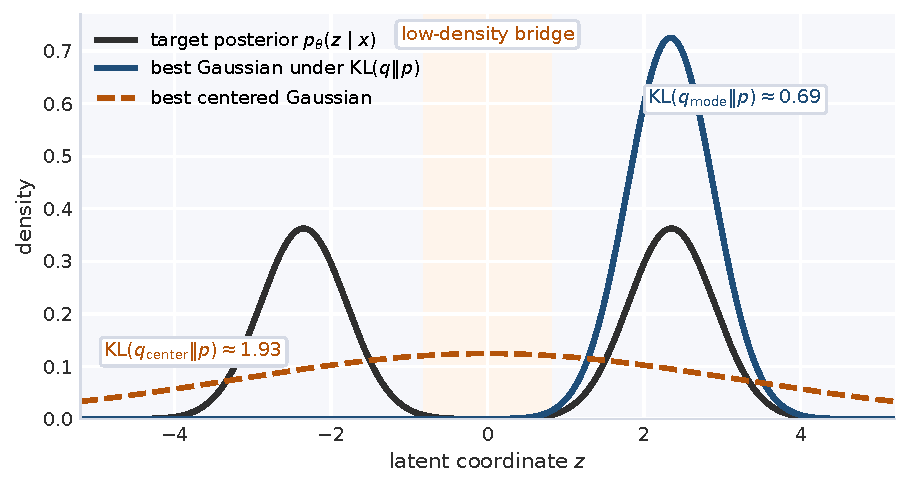
\includegraphics[width=0.92\linewidth]{figures/handouts/elbo_geometry/fig_forward_kl_undercoverage_applied}
  \caption{A bimodal target posterior is approximated by a single Gaussian family.
  The centered Gaussian must place mass in the low-density region between the modes, while the forward-KL minimizer instead concentrates near one mode.
  This is the mode-seeking geometry behind undercoverage.}
  \label{fig:forward-kl-undercoverage-applied}
\end{figure}

In \Cref{fig:forward-kl-undercoverage-applied}, the centered approximation pays for mass throughout the low-density region between the modes, while the forward-KL minimizer avoids that bill and settles on one plausible region.

\begin{exercise}[A three-cell proxy for forward-KL undercoverage]
\label{ex:forward-kl-undercovers}
Approximate a bimodal posterior by three disjoint regions:
\(L\) for the left mode, \(M\) for the low-density middle region, and \(R\) for the right mode.
Suppose
\[
  p(L)=0.49,
  \qquad
  p(M)=0.02,
  \qquad
  p(R)=0.49.
\]
Consider two candidate unimodal approximations:
\[
  q_{\mathrm{mid}}=(0.25,0.50,0.25),
  \qquad
  q_{\mathrm{left}}=(1,0,0),
\]
listed in the order \((L,M,R)\).
\begin{enumerate}[leftmargin=*]
  \item Compute
  \[
    \operatorname{KL}(q_{\mathrm{mid}}\|p)
    =
    \sum_{A\in\{L,M,R\}}
    q_{\mathrm{mid}}(A)\log\frac{q_{\mathrm{mid}}(A)}{p(A)}.
  \]
  \item Compute
  \[
    \operatorname{KL}(q_{\mathrm{left}}\|p).
  \]
  \item Which candidate is preferred by forward KL?
  Explain in one or two sentences which term in the objective makes the centered approximation expensive.
\end{enumerate}
\end{exercise}
\SolutionBox[12]{For the centered candidate,
\[
  \operatorname{KL}(q_{\mathrm{mid}}\|p)
  =
  0.25\log\frac{0.25}{0.49}
  +
  0.50\log\frac{0.50}{0.02}
  +
  0.25\log\frac{0.25}{0.49}
  =
  \frac12\log\frac{625}{49}.
\]
For the left-mode candidate,
\[
  \operatorname{KL}(q_{\mathrm{left}}\|p)
  =
  1\cdot \log\frac{1}{0.49}
  =
  \log\frac{100}{49}.
\]
Numerically,
\[
  \frac12\log\frac{625}{49}\approx 1.27,
  \qquad
  \log\frac{100}{49}\approx 0.71,
\]
so forward KL prefers \(q_{\mathrm{left}}\).
The key penalty is the middle-region term
\[
  0.50\log\frac{0.50}{0.02},
\]
which is large because the centered approximation places substantial mass where the target density is tiny.
This is the discrete version of undercoverage: missing one mode can be cheaper than paying for mass in a low-density middle region.}

The cleanest next example is mean-field VI, where the family deletes dependence before optimization ever starts.

\section{Mean-field deletes dependence before optimization starts}
\label{sec:mean-field-geometry}

\subsection{Factorization is the real approximation}
\label{subsec:mean-field-cavi}

Mean-field VI is the first place where the phrase ``the family is part of the model'' becomes concrete.
Write the latent variable as \(z=(z_1,\dots,z_m)\) and consider the factorized family
\[
  q(z)=\prod_{j=1}^m q_j(z_j).
\]
The point of this choice is not that coordinate ascent is especially deep.
The point is that the posterior is now allowed to move only inside a product geometry.
Any dependence in the true posterior has already been deleted before the optimizer gets to work.

\begin{proposition}[Mean-field coordinate update]
\label{prop:mean-field-update-handout}
Fix all factors except \(q_j\), and assume
\[
  m_j(z_j)\coloneqq \E_{q_{-j}}[\log p_\theta(x,z)]
\]
is finite almost everywhere with \(\int e^{m_j(z_j)}\,dz_j<\infty\).
Then any maximizer of the ELBO over the remaining factor satisfies
\[
  q_j^\star(z_j)
  \propto
  \exp\!\left(
    \E_{q_{-j}}\bigl[\log p_\theta(x,z)\bigr]
  \right),
\]
where the expectation is taken under the current variational law on the remaining coordinates.
\end{proposition}
\begin{proof}
Holding \(q_{-j}\) fixed and optimizing only over \(q_j\), the ELBO becomes
\[
  \mathcal{L}(q;x)
  =
  \int q_j(z_j)\,m_j(z_j)\,dz_j
  -
  \int q_j(z_j)\log q_j(z_j)\,dz_j
  + C,
\]
where \(C\) does not depend on \(q_j\).
Define
\[
  Z_j\coloneqq \int e^{m_j(u)}\,du,
  \qquad
  \widetilde q_j(z_j)\coloneqq Z_j^{-1}e^{m_j(z_j)}.
\]
Then
\[
  \mathcal{L}(q;x)
  =
  -\operatorname{KL}\!\bigl(q_j\,\|\,\widetilde q_j\bigr)+\log Z_j+C,
\]
so the ELBO is maximized at \(q_j=\widetilde q_j\).%
\end{proof}

This is the deterministic analogue of a Gibbs update:
instead of sampling one coordinate from an exact conditional, we replace one factor by the best ELBO fit given the others.
But the more important point is geometric.
Once the family has been factorized, CAVI can only repair the posterior inside that factorized geometry.

\begin{figure}[t]
  \centering
  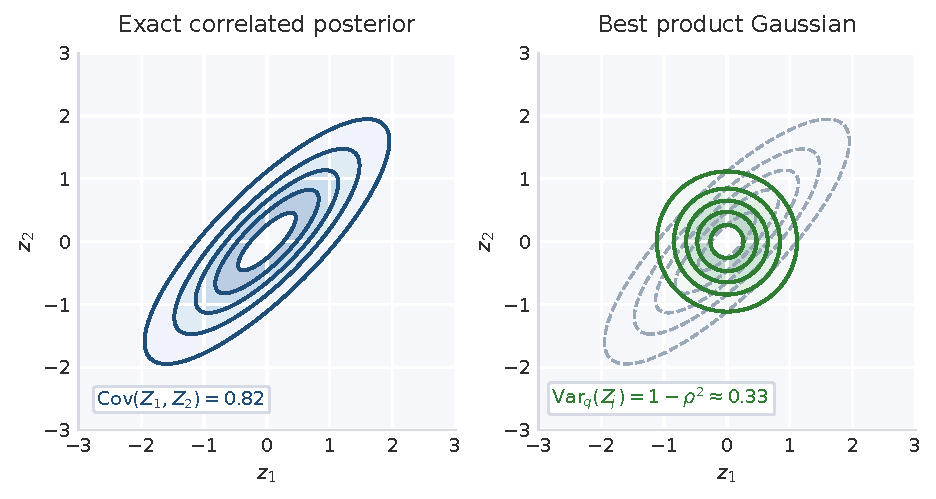
\includegraphics[width=0.92\linewidth]{figures/handouts/elbo_geometry/fig_mean_field_correlation_loss_applied}
  \caption{A correlated Gaussian posterior is compared with the best product Gaussian from the mean-field family.
  The surrogate removes the tilted covariance structure and shrinks each marginal variance, matching the analytic minimizer computed below.}
  \label{fig:mean-field-correlation-loss}
\end{figure}

That loss of geometry is not a training accident.
It is the structural cost of replacing a joint posterior by a product family.
\Cref{fig:mean-field-correlation-loss} shows the cleanest case:
the target posterior is as friendly as possible, but the family is not allowed to tilt.

\begin{proposition}[Best product-Gaussian fit to a correlated Gaussian]
\label{prop:mfvi-gaussian-underdispersion}
Let the exact posterior be
\[
  p_\theta(z\mid x)=\mathcal{N}(0,\Sigma_\rho),
  \qquad
  \Sigma_\rho=
  \begin{bmatrix}
    1 & \rho\\
    \rho & 1
  \end{bmatrix},
  \qquad
  0<|\rho|<1.
\]
Among all fully factorized Gaussian approximations
\[
  q(z_1,z_2)=\mathcal{N}(m_1,s_1^2)\,\mathcal{N}(m_2,s_2^2),
\]
the unique minimizer of
\(\operatorname{KL}(q(z_1,z_2)\|p_\theta(z\mid x))\) satisfies
\[
  m_1=m_2=0,
  \qquad
  s_1^2=s_2^2=1-\rho^2.
\]
In particular, the optimal mean-field approximation is not only uncorrelated; it is also under-dispersed in each coordinate whenever \(\rho\neq 0\).
\end{proposition}
\begin{proof}
The precision matrix is
\[
  \Sigma_\rho^{-1}
  =
  \frac{1}{1-\rho^2}
  \begin{bmatrix}
    1 & -\rho\\
    -\rho & 1
  \end{bmatrix}.
\]
A direct Gaussian-KL calculation gives
\[
  \operatorname{KL}(q\|p_\theta(\cdot\mid x))
  =
  \frac12\left[
    \frac{m_1^2-2\rho m_1m_2+m_2^2+s_1^2+s_2^2}{1-\rho^2}
    -2
    +
    \log\!\frac{1-\rho^2}{s_1^2s_2^2}
  \right].
\]
The quadratic form in \((m_1,m_2)\) is minimized uniquely at \(m_1=m_2=0\).
For \(j\in\{1,2\}\),
\[
  \frac{\partial}{\partial s_j^2}\operatorname{KL}(q\|p_\theta(\cdot\mid x))
  =
  \frac12\left(\frac{1}{1-\rho^2}-\frac{1}{s_j^2}\right),
\]
so the unique stationary point is \(s_j^2=1-\rho^2\).
Since the second derivative with respect to \(s_j^2\) is \(1/(2s_j^4)>0\), this stationary point is the global minimizer.%
\end{proof}

This calculation says exactly what the picture suggests.
The best product approximation cannot reproduce the tilted covariance geometry, so it compensates by shrinking the marginal variances.
Even in the Gaussian case, forward KL plus factorization produces an axis-aligned, overconfident surrogate.

\begin{exercise}[Recover the best product Gaussian]
\label{ex:mean-field-removes-dependence}
Use the displayed formula
\[
  \operatorname{KL}(q\|p_\theta(\cdot\mid x))
  =
  \frac12\left[
    \frac{m_1^2-2\rho m_1m_2+m_2^2+s_1^2+s_2^2}{1-\rho^2}
    -2
    +
    \log\!\frac{1-\rho^2}{s_1^2s_2^2}
  \right]
\]
for the factorized Gaussian \(q(z)=\mathcal{N}(m_1,s_1^2)\mathcal{N}(m_2,s_2^2)\).
\begin{enumerate}[leftmargin=*]
  \item Holding \(s_1^2,s_2^2\) fixed, differentiate with respect to \(m_1,m_2\) and show that the unique stationary point is \(m_1=m_2=0\).
  \item Differentiate with respect to \(s_1^2\) and \(s_2^2\) and show that the minimizer satisfies
  \[
    s_1^2=s_2^2=1-\rho^2.
  \]
  \item Compare these values with the exact posterior variances and covariance. What two geometric distortions does the best product approximation impose?
\end{enumerate}
\end{exercise}
\SolutionBox[12]{Differentiating the KL with respect to the means gives
\[
  \frac{\partial}{\partial m_1}\operatorname{KL}(q\|p_\theta(\cdot\mid x))
  =
  \frac{m_1-\rho m_2}{1-\rho^2},
  \qquad
  \frac{\partial}{\partial m_2}\operatorname{KL}(q\|p_\theta(\cdot\mid x))
  =
  \frac{m_2-\rho m_1}{1-\rho^2}.
\]
The stationary conditions are
\[
  m_1=\rho m_2,
  \qquad
  m_2=\rho m_1.
\]
Since \(|\rho|<1\), the unique solution is \(m_1=m_2=0\).
For the variances,
\[
  \frac{\partial}{\partial s_j^2}\operatorname{KL}(q\|p_\theta(\cdot\mid x))
  =
  \frac12\left(\frac{1}{1-\rho^2}-\frac{1}{s_j^2}\right),
  \qquad j\in\{1,2\},
\]
so the stationary point is \(s_1^2=s_2^2=1-\rho^2\), which is the minimizer.
The exact posterior has marginal variances \(1\) and covariance \(\rho\), while the best product approximation has variances \(1-\rho^2<1\) and covariance \(0\).
So mean-field imposes two distortions at once: it deletes posterior dependence and it shrinks each marginal variance below the true one.}

Up to this point every failure has been local:
one observation, one posterior, one restricted family.
Amortization adds a second restriction across data.

\section{Shared encoders and one latent bottleneck}
\label{sec:shared-encoder-bottleneck}

\subsection{Amortization adds a second restriction}
\label{subsec:amortization-gap}

Amortized VI replaces per-datum variational optimization by a shared encoder \(q_\phi(z\mid x)\).
That makes inference scalable, but it also means that all posterior approximations must lie on the image of one learned map \(x\mapsto q_\phi(\cdot\mid x)\).
On a data set \(x_1,\dots,x_n\), the optimization problem becomes
\[
  \max_{\phi\in\Phi}\sum_{i=1}^n \mathcal{L}(q_\phi(\cdot\mid x_i);x_i)
  \qquad\text{instead of}\qquad
  \sum_{i=1}^n \max_{q\in\mathcal{Q}} \mathcal{L}(q;x_i).
\]
So amortization is not just a faster optimizer for the same approximation problem.
It is a smaller approximation problem.

\begin{figure}[t]
  \centering
  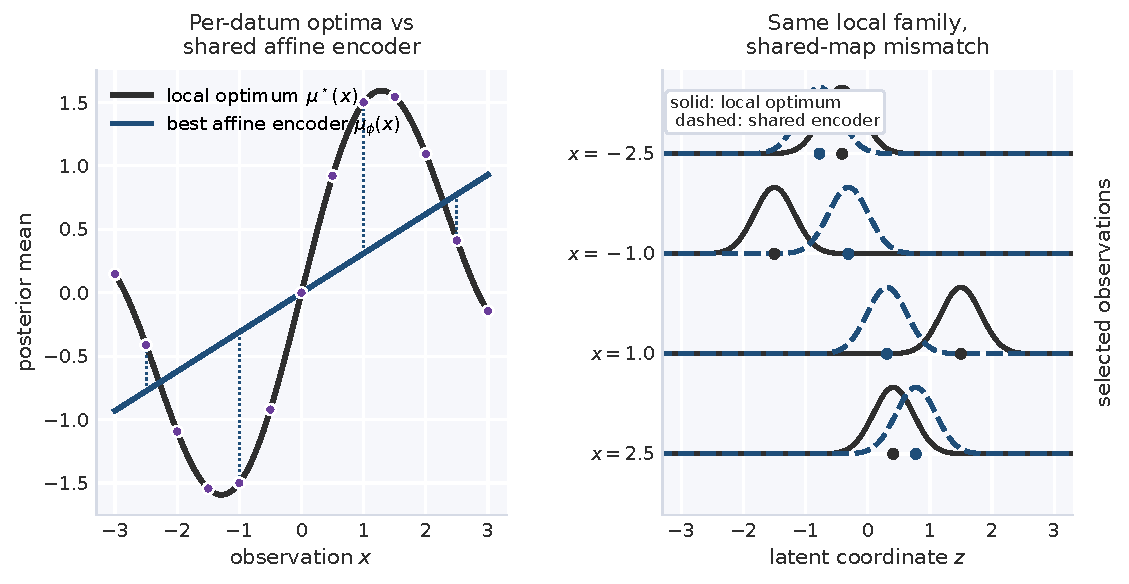
\includegraphics[width=\linewidth]{figures/handouts/elbo_geometry/fig_vi_amortization_applied}
  \caption{A synthetic posterior family with nonlinear per-datum optima \(\mu^\star(x)\) is approximated by a shared affine encoder family.
  The local posteriors are individually representable, but one shared map cannot hit all of the targets simultaneously.
  This is the amortization gap.}
  \label{fig:vi-amortization-handout}
\end{figure}

\Cref{fig:vi-amortization-handout} separates two failure modes that are easy to conflate.
The local family may be adequate for each datum, yet the shared encoder may still miss the local optimum because one map cannot bend in all the required directions at once.

\begin{proposition}[Amortization cannot beat per-datum variational optima]
\label{prop:amortization-gap}
Let \(x_1,\dots,x_n\) be observations, and let \(\mathcal{Q}\) be a variational family available for each datum individually.
Define
\[
  \mathcal{L}_i^\star \coloneqq \sup_{q\in\mathcal{Q}} \mathcal{L}(q;x_i).
\]
Then for any amortized family \(\{q_\phi(\cdot\mid x):\phi\in\Phi\}\subseteq \mathcal{Q}\),
\[
  \sup_{\phi\in\Phi} \sum_{i=1}^n \mathcal{L}(q_\phi(\cdot\mid x_i);x_i)
  \le
  \sum_{i=1}^n \mathcal{L}_i^\star.
\]
\end{proposition}
\begin{proof}
Fix \(\phi\).
For each \(i\), the distribution \(q_\phi(\cdot\mid x_i)\) belongs to \(\mathcal{Q}\), so
\[
  \mathcal{L}(q_\phi(\cdot\mid x_i);x_i)\le \mathcal{L}_i^\star.
\]
Summing over \(i\) gives
\[
  \sum_{i=1}^n \mathcal{L}(q_\phi(\cdot\mid x_i);x_i)\le \sum_{i=1}^n \mathcal{L}_i^\star.
\]
Taking the supremum over \(\phi\) preserves the inequality.%
\end{proof}

The proposition is simple, but it is the correct formal separation between family mismatch and amortization gap.
The gap vanishes only if one shared encoder hits the per-datum optimum everywhere.
Computationally, amortization is still the right idea:
the recognition model and the reparameterized gradient estimator from AEVB and stochastic backpropagation make \(\mathcal{J}(\theta,\phi)\) trainable at scale
\citep[\S\S2.1--2.3]{kingma_welling_2014_aevb}
\citep[\S\S1, 3]{rezende_mohamed_wierstra_2014_stochastic_backpropagation}.
But neither device removes the underlying geometric restriction.

\begin{exercise}[Decompose local mismatch and amortization gap]
\label{ex:amortization-gap}
Let
\[
  \mathcal{L}_i^\star
  \coloneqq
  \sup_{q\in\mathcal{Q}}\mathcal{L}(q;x_i),
  \qquad i=1,\dots,n.
\]
Define the local approximation gap
\[
  \Delta_i^{\mathrm{loc}}
  \coloneqq
  \log p_\theta(x_i)-\mathcal{L}_i^\star
\]
and the amortization gap
\[
  \Delta_{\mathrm{am}}
  \coloneqq
  \sum_{i=1}^n \mathcal{L}_i^\star
  -
  \sup_{\phi\in\Phi}\sum_{i=1}^n \mathcal{L}(q_\phi(\cdot\mid x_i);x_i).
\]
Assume the amortized family satisfies
\[
  \{q_\phi(\cdot\mid x_i):\phi\in\Phi\}\subseteq \mathcal{Q}
  \qquad\text{for every }i.
\]
\begin{enumerate}[leftmargin=*]
  \item Use the ELBO--KL identity to show that, for each \(i\),
  \[
    \Delta_i^{\mathrm{loc}}
    =
    \inf_{q\in\mathcal{Q}}
    \operatorname{KL}\!\bigl(q(z)\,\|\,p_\theta(z\mid x_i)\bigr),
  \]
  and in particular \(\Delta_i^{\mathrm{loc}}\ge 0\).
  \item Use \Cref{prop:amortization-gap} to show \(\Delta_{\mathrm{am}}\ge 0\).
  \item Fix \(\phi\). Show that for each \(i\),
  \[
    \mathcal{L}(q_\phi(\cdot\mid x_i);x_i)\le \mathcal{L}_i^\star.
  \]
  Then sum over \(i\) and take the supremum over \(\phi\) to recover the inequality
  \[
    \sup_{\phi\in\Phi}\sum_{i=1}^n \mathcal{L}(q_\phi(\cdot\mid x_i);x_i)
    \le
    \sum_{i=1}^n \mathcal{L}_i^\star.
  \]
  \item Prove the exact decomposition
  \[
    \sum_{i=1}^n \log p_\theta(x_i)
    -
    \sup_{\phi\in\Phi}\sum_{i=1}^n \mathcal{L}(q_\phi(\cdot\mid x_i);x_i)
    =
    \sum_{i=1}^n \Delta_i^{\mathrm{loc}}
    +
    \Delta_{\mathrm{am}}.
  \]
  \item Explain what vanishes in the two extreme cases:
  a purely local-family-limited regime and a purely amortization-limited regime.
\end{enumerate}
\end{exercise}
\SolutionBox[15]{By the ELBO--KL identity,
\[
  \log p_\theta(x_i)
  =
  \mathcal{L}(q;x_i)
  +
  \operatorname{KL}\!\bigl(q(z)\,\|\,p_\theta(z\mid x_i)\bigr)
\]
for every admissible \(q\in\mathcal{Q}\).
Taking the supremum over \(q\in\mathcal{Q}\) on the ELBO side is the same as taking the infimum of the KL term, so
\[
  \Delta_i^{\mathrm{loc}}
  =
  \log p_\theta(x_i)-\mathcal{L}_i^\star
  =
  \inf_{q\in\mathcal{Q}}
  \operatorname{KL}\!\bigl(q(z)\,\|\,p_\theta(z\mid x_i)\bigr)\ge 0.
\]
Next,
\[
  \Delta_{\mathrm{am}}
  =
  \sum_{i=1}^n \mathcal{L}_i^\star
  -
  \sup_{\phi\in\Phi}\sum_{i=1}^n \mathcal{L}(q_\phi(\cdot\mid x_i);x_i)\ge 0
\]
by \Cref{prop:amortization-gap}.
Fix \(\phi\).
For each datum \(x_i\), the distribution \(q_\phi(\cdot\mid x_i)\) belongs to \(\mathcal{Q}\), so by definition of \(\mathcal{L}_i^\star\),
\[
  \mathcal{L}(q_\phi(\cdot\mid x_i);x_i)\le \mathcal{L}_i^\star.
\]
Summing over \(i\) gives
\[
  \sum_{i=1}^n \mathcal{L}(q_\phi(\cdot\mid x_i);x_i)
  \le
  \sum_{i=1}^n \mathcal{L}_i^\star.
\]
Taking the supremum over \(\phi\) preserves the inequality and yields the claim.
For the exact decomposition, add and subtract \(\sum_i \mathcal{L}_i^\star\):
\begin{align*}
  \sum_{i=1}^n \log p_\theta(x_i)
  -
  \sup_{\phi}\sum_{i=1}^n \mathcal{L}(q_\phi(\cdot\mid x_i);x_i)
  &=
  \sum_{i=1}^n \bigl(\log p_\theta(x_i)-\mathcal{L}_i^\star\bigr) \\
  &\quad
  +
  \sum_{i=1}^n \mathcal{L}_i^\star
  -
  \sup_{\phi}\sum_{i=1}^n \mathcal{L}(q_\phi(\cdot\mid x_i);x_i) \\
  &=
  \sum_{i=1}^n \Delta_i^{\mathrm{loc}}+\Delta_{\mathrm{am}}.
\end{align*}
In a purely local-family-limited regime, \(\Delta_{\mathrm{am}}=0\) and the whole gap comes from the local family \(\mathcal{Q}\) being too small.
In a purely amortization-limited regime, every \(\Delta_i^{\mathrm{loc}}=0\) and the whole gap comes from one shared encoder failing to realize the per-datum optima.}

\subsection{Blur: overlapping latent neighborhoods force averaging}
\label{subsec:blur}

From this point on, keep the standard one-bottleneck VAE in mind:
a prior \(p(z)\), decoder \(p_\theta(x\mid z)\), and shared encoder \(q_\phi(z\mid x)\).
This is the AEVB setting with the usual reparameterization
\[
  z=\mu_\phi(x)+\sigma_\phi(x)\odot \varepsilon,
  \qquad
  \varepsilon\sim\mathcal{N}(0,I),
\]
which makes stochastic ELBO optimization practical but does not alter the geometry of the approximation problem
\citep[\S\S2.1--2.3]{kingma_welling_2014_aevb}
\citep[\S3]{rezende_mohamed_wierstra_2014_stochastic_backpropagation}.

The blur mechanism becomes sharp when the decoder is Gaussian.
Then, for fixed \(q_\phi\), decoder learning is literally a regression problem under the joint law induced by the data and the encoder.
That is the direct link from ``posterior overlap'' to blurry reconstructions.

\begin{proposition}[A fixed-encoder Gaussian VAE is regression under \(p_{\mathrm{data}}(x)q_\phi(z\mid x)\)]
\label{prop:gaussian-vae-regression}
Assume \(\sigma^2>0\) is fixed and
\[
  p_\theta(x\mid z)=\mathcal{N}\!\bigl(\mu_\theta(z),\sigma^2 I\bigr).
\]
Then the expected ELBO over the data distribution satisfies
\[
  \E_{p_{\mathrm{data}}(x)}\!\bigl[\mathcal{L}(q_\phi;x)\bigr]
  =
  C(\phi,\sigma^2)
  -
  \frac{1}{2\sigma^2}
  \E_{(X,Z)\sim \pi_\phi}\!\bigl[\norm{X-\mu_\theta(Z)}_2^2\bigr],
\]
where
\[
  \pi_\phi(dx,dz)\coloneqq p_{\mathrm{data}}(x)\,q_\phi(dz\mid x)
\]
and
\[
  C(\phi,\sigma^2)
  =
  -\frac{d}{2}\log(2\pi\sigma^2)
  -
  \E_{p_{\mathrm{data}}(x)}
  \operatorname{KL}\!\bigl(q_\phi(z\mid x)\,\|\,p(z)\bigr)
\]
does not depend on \(\mu_\theta\).
Consequently, for fixed \(q_\phi\), maximizing the expected ELBO over decoder means \(\mu_\theta\) is equivalent to minimizing
\[
  \mu\mapsto
  \E_{(X,Z)\sim \pi_\phi}\!\bigl[\norm{X-\mu(Z)}_2^2\bigr].
\]
\end{proposition}
\begin{proof}
For each \(x\),
\[
  \mathcal{L}(q_\phi;x)
  =
  \E_{q_\phi(z\mid x)}[\log p_\theta(x\mid z)]
  -
  \operatorname{KL}\!\bigl(q_\phi(z\mid x)\,\|\,p(z)\bigr).
\]
Under the Gaussian decoder,
\[
  \log p_\theta(x\mid z)
  =
  -\frac{d}{2}\log(2\pi\sigma^2)
  -
  \frac{1}{2\sigma^2}\norm{x-\mu_\theta(z)}_2^2.
\]
Taking expectations over \(p_{\mathrm{data}}(x)\) gives
\begin{align*}
  \E_{p_{\mathrm{data}}(x)}\!\bigl[\mathcal{L}(q_\phi;x)\bigr]
  &=
  -\frac{d}{2}\log(2\pi\sigma^2)
  -
  \frac{1}{2\sigma^2}
  \E_{p_{\mathrm{data}}(x)q_\phi(z\mid x)}
  \norm{x-\mu_\theta(z)}_2^2 \\
  &\quad
  -
  \E_{p_{\mathrm{data}}(x)}
  \operatorname{KL}\!\bigl(q_\phi(z\mid x)\,\|\,p(z)\bigr),
\end{align*}
which is the stated identity.%
\end{proof}

\begin{proposition}[Squared loss chooses conditional means]
\label{prop:squared-error-mean}
Let \((X,Z)\) be jointly distributed with \(X\in\R^d\), \(Z\in\R^m\), and \(\E\norm{X}_2^2<\infty\).
Among all measurable maps \(\mu:\R^m\to\R^d\) such that \(\E\norm{\mu(Z)}_2^2<\infty\), the minimizer of
\[
  \mu\mapsto \E\norm{X-\mu(Z)}_2^2
\]
satisfies
\[
  \mu^\star(Z)=\E[X\mid Z]
\]
almost surely, where \(\E[X\mid Z]\) denotes any version of the conditional expectation.
\end{proposition}
\begin{proof}
For any measurable \(\mu\),
\begin{align*}
  \E\norm{X-\mu(Z)}_2^2
  &=
  \E\norm{X-\E[X\mid Z]}_2^2
  +
  \E\norm{\E[X\mid Z]-\mu(Z)}_2^2 \\
  &\quad
  +
  2\,\E\!\left[
    \ip{X-\E[X\mid Z]}{\E[X\mid Z]-\mu(Z)}
  \right].
\end{align*}
The cross term vanishes because
\[
  \E\!\left[X-\E[X\mid Z]\mid Z\right]=0
\]
and \(\E[X\mid Z]-\mu(Z)\) is \(Z\)-measurable.
Therefore
\[
  \E\norm{X-\mu(Z)}_2^2
  =
  \E\norm{X-\E[X\mid Z]}_2^2
  +
  \E\norm{\E[X\mid Z]-\mu(Z)}_2^2,
\]
so the minimum is attained exactly when \(\mu(Z)=\E[X\mid Z]\) almost surely.%
\end{proof}

\Cref{prop:gaussian-vae-regression} and \Cref{prop:squared-error-mean} give the blur mechanism in one line:
for fixed \(q_\phi\), a Gaussian decoder mean that minimizes the reconstruction risk is any version of
\[
  \mu_\theta^\star(Z)=\E_{\pi_\phi}[X\mid Z]
\]
almost surely.
So if the encoder geometry pushes several incompatible observations into the same latent neighborhood, the decoder is forced toward a conditional mean rather than any one sharp sample.
This makes precise the ``posterior overlap'' and ``locality'' story emphasized in the \(\beta\)-VAE discussion of \citet[\S\S4.2--5]{burgess_higgins_pal_matthey_watters_desjardins_lerchner_2018_understanding_bvae}.

\subsubsection{A two-point blur example}
\label{subsubsec:two-point-blur}

The abstract conditional-mean statement becomes concrete in the smallest nontrivial example.
If one latent neighborhood mixes two genuinely different observations, the decoder has no sharper target available than their average.

\begin{example}[Ambiguity forces averaging]
\label{ex:two-point-blur}
Suppose the data distribution places probability \(1/2\) on \(x^{(1)}\in\R^d\) and probability \(1/2\) on \(x^{(2)}\in\R^d\), and suppose that a version of the conditional law of \(X\) given \(Z\) satisfies, at some latent location \(z\),
\[
  \Pr(X=x^{(1)}\mid Z=z)
  =
  \Pr(X=x^{(2)}\mid Z=z)
  =
  \frac12.
\]
Then a risk-minimizing Gaussian-decoder prediction at that latent point is
\[
  \mu_\theta(z)
  =
  \E[X\mid Z=z]
  =
  \frac{x^{(1)}+x^{(2)}}{2}.
\]
Unless \(x^{(1)}=x^{(2)}\), the reconstruction is an average rather than an actual datum.
\end{example}

The example is tiny, but it captures the full story.
Blur does not mean the decoder is inherently bad at detail.
It means the encoder geometry failed to separate distinctions that matter to squared-error reconstruction.
When the bottleneck has too little effective capacity, the decoder is rewarded for averaging unresolved variation
\citep[\S\S4.2--5]{burgess_higgins_pal_matthey_watters_desjardins_lerchner_2018_understanding_bvae}.

\begin{figure}[t]
  \centering
  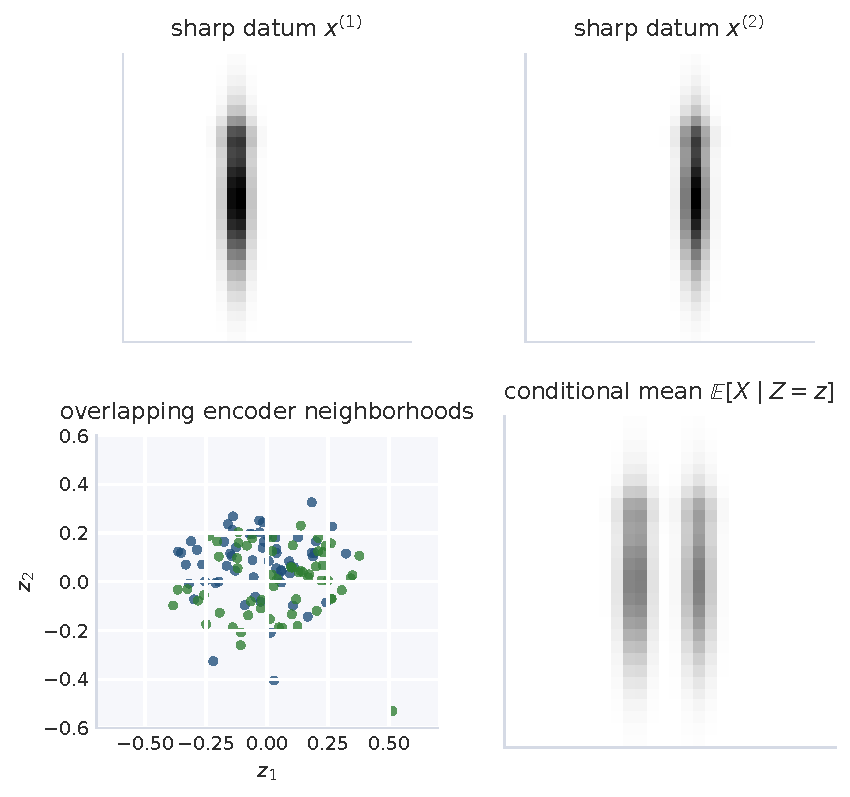
\includegraphics[width=0.84\linewidth]{figures/handouts/elbo_geometry/fig_latent_overlap_blur_applied}
  \caption{Two distinct sharp observations are mapped into nearly the same latent neighborhood.
  A Gaussian decoder therefore returns their conditional mean, which is visibly blurrier than either endpoint.}
  \label{fig:latent-overlap-blur}
\end{figure}

\begin{exercise}[The irreducible blur penalty]
\label{ex:blur-average}
In the two-point example above, show the exact identity
\[
  \frac12\norm{x^{(1)}-a}_2^2+\frac12\norm{x^{(2)}-a}_2^2
  =
  \frac14\norm{x^{(1)}-x^{(2)}}_2^2
  +
  \norm{a-\tfrac12(x^{(1)}+x^{(2)})}_2^2.
\]
Deduce that the minimizer is \(a=(x^{(1)}+x^{(2)})/2\) and compute the minimum value explicitly in terms of \(\norm{x^{(1)}-x^{(2)}}_2\).
Then explain how this finite identity mirrors the decomposition in \Cref{prop:squared-error-mean}.
\end{exercise}
\SolutionBox[9]{Expanding the quadratic gives
\[
  \frac12\norm{x^{(1)}-a}_2^2+\frac12\norm{x^{(2)}-a}_2^2
  =
  \frac14\norm{x^{(1)}-x^{(2)}}_2^2
  +
  \norm{a-\tfrac12(x^{(1)}+x^{(2)})}_2^2.
\]
Hence the minimizer is the midpoint \(a=(x^{(1)}+x^{(2)})/2\).
The minimum value is
\[
  \frac14\norm{x^{(1)}-x^{(2)}}_2^2.
\]
This is the two-point version of \Cref{prop:squared-error-mean}: the first term is the irreducible conditional-variance cost, and the second term is the extra penalty for choosing a prediction different from the conditional mean.
So even the best decoder incurs a positive reconstruction penalty whenever distinct observations share one latent code.}

\subsection{Collapse: the decoder can make latent information too expensive}
\label{subsec:collapse}

Blur and collapse are opposite-looking symptoms of the same bottleneck picture.
In blur, the latent code is used but is not expressive enough to separate incompatible observations.
In collapse, the decoder becomes so strong that using \(z\) is not worth the KL bill.
The cleanest formal toy case is when the decoder literally ignores \(z\).

\begin{proposition}[If the decoder ignores \(z\), the ELBO prefers the prior]
\label{prop:collapse-if-decoder-ignores-z}
Suppose \(p_\theta(x\mid z)=p_\theta(x)\) for all \(z\).
Then for every \(x\),
\[
  \mathcal{L}(q;x)=\log p_\theta(x)-\operatorname{KL}\!\bigl(q(z)\,\|\,p(z)\bigr),
\]
so the ELBO is maximized by \(q(z)=p(z)\).
\end{proposition}
\begin{proof}
Under the assumption \(p_\theta(x\mid z)=p_\theta(x)\),
\[
  p_\theta(x,z)=p_\theta(x)\,p(z).
\]
Substituting this into the ELBO gives
\[
  \mathcal{L}(q;x)
  =
  \E_q[\log p_\theta(x)+\log p(z)-\log q(z)]
  =
  \log p_\theta(x)-\operatorname{KL}\!\bigl(q(z)\,\|\,p(z)\bigr).
\]
The KL term is minimized at \(q(z)=p(z)\), proving the claim.%
\end{proof}

Real posterior collapse is usually less extreme than this toy case, but the geometry is the same.
If the decoder can already explain \(x\) well enough on its own, then the ELBO charges for transmitting information through \(z\) without demanding much in return.
The latent variable becomes expendable.

To see the bill more clearly, average the KL term over the data distribution and define the aggregate posterior
\[
  q_\phi(z)
  \coloneqq
  \int q_\phi(z\mid x)\,p_{\mathrm{data}}(x)\,dx.
\]

\begin{proposition}[Mutual-information decomposition of the KL term]
\label{prop:mi-decomposition}
Assume \(q_\phi(z\mid x)\) and \(p(z)\) are densities with respect to a common base measure and that the displayed expectations are finite.
We have
\[
  \E_{p_{\mathrm{data}}(x)}
  \operatorname{KL}\!\bigl(q_\phi(z\mid x)\,\|\,p(z)\bigr)
  =
  I_q(X;Z)
  +
  \operatorname{KL}\!\bigl(q_\phi(z)\,\|\,p(z)\bigr),
\]
where \(I_q(X;Z)\) is mutual information under the joint law
\[
  p_{\mathrm{data}}(x)\,q_\phi(z\mid x).
\]
\end{proposition}
\begin{proof}
Expand the left-hand side:
\[
  \E_{p_{\mathrm{data}}(x)q_\phi(z\mid x)}
  \bigl[\log q_\phi(z\mid x)-\log p(z)\bigr].
\]
Add and subtract \(\log q_\phi(z)\):
\[
  \E\!\bigl[\log q_\phi(z\mid x)-\log q_\phi(z)\bigr]
  +
  \E\!\bigl[\log q_\phi(z)-\log p(z)\bigr].
\]
The first term is \(I_q(X;Z)\), and the second is
\(\operatorname{KL}(q_\phi(z)\|p(z))\).%
\end{proof}

Combining \Cref{prop:mi-decomposition} with the expected ELBO gives
\[
  \E_{p_{\mathrm{data}}(x)}\!\bigl[\mathcal{L}(q_\phi;x)\bigr]
  =
  \E_{p_{\mathrm{data}}(x)q_\phi(z\mid x)}[\log p_\theta(x\mid z)]
  -
  I_q(X;Z)
  -
  \operatorname{KL}\!\bigl(q_\phi(z)\,\|\,p(z)\bigr).
\]
So the KL regularizer is charging for two things at once:
how much information the code stores about the data, and how far the aggregate code distribution drifts from the prior.
If the decoder class already contains good nearly unconditional models for the data, the collapsed solution can be globally competitive; more generally, using \(z\) is worthwhile only when the reconstruction gain beats this information bill.

This helps explain why expressive autoregressive decoders often collapse in practice.
Bowman et al.\ show the sentence-VAE version of this story:
if the decoder is already a strong language model, training pushes \(q_\phi(z\mid x)\) back toward the prior unless the optimization pressure is modified
\citep[\S3.1]{bowman_vilnis_vinyals_dai_jozefowicz_bengio_2016_generating_sentences}.
He et al.\ give the complementary dynamic explanation:
early in training the decoder can move faster than the inference network, and that lag can steer the system into a collapsed regime before the encoder learns to use \(z\)
\citep[\S\S3--4]{he_spokoyny_neubig_bergkirkpatrick_2019_lagging_inference}.

\begin{figure}[t]
  \centering
  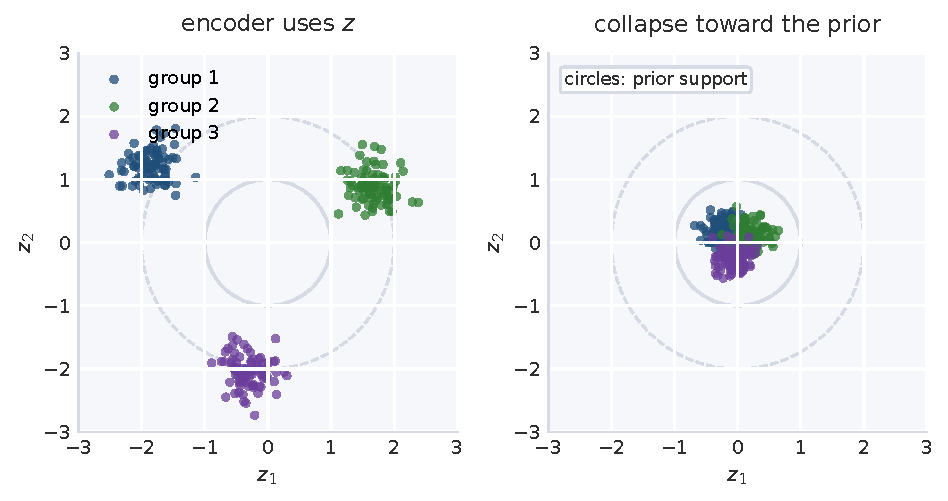
\includegraphics[width=0.90\linewidth]{figures/handouts/elbo_geometry/fig_decoder_bypass_collapse_applied}
  \caption{Toy encoder outputs for three groups of observations.
  When the latent variable is used, the group-conditioned posteriors separate in latent space; under posterior collapse they contract back toward the prior and overlap heavily, so little information about \(x\) remains in \(z\).}
  \label{fig:decoder-bypass-collapse}
\end{figure}

This also clarifies what KL warm-up and \(\beta\)-VAE style heuristics do.
They change the price of information.
That can change which local optimum training reaches, but it does not enlarge the variational family or remove the possibility of collapse
\citep[\S3.1]{bowman_vilnis_vinyals_dai_jozefowicz_bengio_2016_generating_sentences}
\citep[\S\S3--5]{burgess_higgins_pal_matthey_watters_desjardins_lerchner_2018_understanding_bvae}.

\begin{exercise}[\(\beta\)-ELBO as a weighted information budget]
\label{ex:beta-elbo}
Consider the \(\beta\)-ELBO
\[
  \mathcal{L}_\beta(q;x)
  =
  \E_q[\log p_\theta(x\mid z)]
  -
  \beta\,\operatorname{KL}\!\bigl(q(z)\,\|\,p(z)\bigr).
\]
\begin{enumerate}[leftmargin=*]
  \item After averaging over \(p_{\mathrm{data}}(x)\), write the objective as
  \[
    \E_{p_{\mathrm{data}}(x)q_\phi(z\mid x)}[\log p_\theta(x\mid z)]
    -
    \beta\,\E_{p_{\mathrm{data}}(x)}
    \operatorname{KL}\!\bigl(q_\phi(z\mid x)\,\|\,p(z)\bigr).
  \]
  \item In the averaged KL term, add and subtract \(\log q_\phi(z)\) exactly as in the proof of \Cref{prop:mi-decomposition}.
  \item Identify the two resulting terms and conclude that
  \[
    \E_{p_{\mathrm{data}}(x)}[\mathcal{L}_\beta(q_\phi;x)]
    =
    \E_{p_{\mathrm{data}}(x)q_\phi(z\mid x)}[\log p_\theta(x\mid z)]
    -
    \beta\,I_q(X;Z)
    -
    \beta\,\operatorname{KL}\!\bigl(q_\phi(z)\,\|\,p(z)\bigr).
  \]
  \item State separately what large \(\beta\) and small \(\beta\) do to the two non-reconstruction terms.
\end{enumerate}
\end{exercise}
\SolutionBox[10]{Apply \Cref{prop:mi-decomposition} to the averaged KL term:
\[
  \E_{p_{\mathrm{data}}(x)}
  \operatorname{KL}\!\bigl(q_\phi(z\mid x)\,\|\,p(z)\bigr)
  =
  I_q(X;Z)
  +
  \operatorname{KL}\!\bigl(q_\phi(z)\,\|\,p(z)\bigr).
\]
More explicitly,
\[
  \E\!\bigl[\log q_\phi(z\mid x)-\log p(z)\bigr]
  =
  \E\!\bigl[\log q_\phi(z\mid x)-\log q_\phi(z)\bigr]
  +
  \E\!\bigl[\log q_\phi(z)-\log p(z)\bigr],
\]
where the first expectation is \(I_q(X;Z)\) and the second is
\(\operatorname{KL}(q_\phi(z)\|p(z))\).
Substituting into the expected \(\beta\)-ELBO yields
\[
  \E_{p_{\mathrm{data}}(x)}[\mathcal{L}_\beta(q_\phi;x)]
  =
  \E_{p_{\mathrm{data}}(x)q_\phi(z\mid x)}[\log p_\theta(x\mid z)]
  -
  \beta\,I_q(X;Z)
  -
  \beta\,\operatorname{KL}\!\bigl(q_\phi(z)\,\|\,p(z)\bigr).
\]
So \(\beta\) directly rescales both parts of the KL bill.
Large \(\beta\) makes informative codes and prior mismatch expensive, which pushes toward weaker latent usage and can favor collapse.
Small \(\beta\) relaxes both penalties, so the model is more willing to store information in \(z\) and to let the aggregate posterior drift from the prior.
This changes optimization pressure, but it does not enlarge the family \(q_\phi(z\mid x)\), so it does not remove the underlying geometric mismatch.}

\section{Structural redesigns}
\label{sec:structural-redesigns}

Once the problem is framed this way, the right fix is often not ``optimize the same ELBO harder''.
If one latent layer is too coarse, or if learning the encoder geometry itself is unstable, then the approximation problem must change.
Two recurring redesigns do that:
hierarchy and fixed-bridge latent models.

\subsection{Hierarchy splits one overloaded KL bill into local bills}
\label{subsec:hierarchy-redistributes-kl}

A hierarchical VAE replaces one bottleneck by a stack of latent variables.
The key point is not just that the network is deeper.
The important change is that no single latent variable has to pay for every kind of variation at once.
Coarse structure can be represented high in the hierarchy and local detail lower down, so the ELBO decomposes into several local KL penalties instead of one global bottleneck charge.

Consider a hierarchical VAE with latent variables \(z_{1:L}\) and factorization
\[
  p_\theta(x,z_{1:L})
  =
  p_\theta(x\mid z_1)\,
  \prod_{\ell=1}^{L-1} p_\theta(z_\ell\mid z_{\ell+1})\,
  p(z_L),
\]
together with a structured encoder
\[
  q_\phi(z_{1:L}\mid x)
  =
  q_\phi(z_L\mid x)\,
  \prod_{\ell=1}^{L-1} q_\phi(z_\ell\mid z_{\ell+1},x).
\]

\begin{proposition}[Hierarchical ELBO as reconstruction minus local KL terms]
\label{prop:hierarchical-elbo}
For the model and encoder above,
\begin{align*}
  \mathcal{L}(q_\phi;x)
  &=
  \E_{q_\phi}\bigl[\log p_\theta(x\mid z_1)\bigr]
  -
  \operatorname{KL}\!\bigl(q_\phi(z_L\mid x)\,\|\,p(z_L)\bigr) \\
  &\quad
  -
  \sum_{\ell=1}^{L-1}
  \E_{q_\phi(z_{\ell+1:L}\mid x)}\!\left[
    \operatorname{KL}\!\bigl(
      q_\phi(z_\ell\mid z_{\ell+1},x)\,\|\,p_\theta(z_\ell\mid z_{\ell+1})
    \bigr)
  \right].
\end{align*}
\end{proposition}
\begin{proof}
Start from
\[
  \mathcal{L}(q_\phi;x)
  =
  \E_{q_\phi}\!\bigl[\log p_\theta(x,z_{1:L})-\log q_\phi(z_{1:L}\mid x)\bigr].
\]
Substituting the factorizations of \(p_\theta\) and \(q_\phi\) gives
\begin{align*}
  \mathcal{L}(q_\phi;x)
  &=
  \E_{q_\phi}[\log p_\theta(x\mid z_1)] \\
  &\quad
  +
  \E_{q_\phi}\!\left[
    \sum_{\ell=1}^{L-1} \log p_\theta(z_\ell\mid z_{\ell+1})
    + \log p(z_L)
    - \sum_{\ell=1}^{L-1} \log q_\phi(z_\ell\mid z_{\ell+1},x)
    - \log q_\phi(z_L\mid x)
  \right].
\end{align*}
The top-level terms combine as
\[
  \E_{q_\phi}\!\left[\log p(z_L)-\log q_\phi(z_L\mid x)\right]
  =
  -\operatorname{KL}\!\bigl(q_\phi(z_L\mid x)\,\|\,p(z_L)\bigr).
\]
For each \(\ell\in\{1,\dots,L-1\}\),
\begin{align*}
  &\E_{q_\phi}\!\left[
    \log p_\theta(z_\ell\mid z_{\ell+1})
    -
    \log q_\phi(z_\ell\mid z_{\ell+1},x)
  \right] \\
  &\qquad
  =
  -\E_{q_\phi(z_{\ell+1:L}\mid x)}\!\left[
    \operatorname{KL}\!\bigl(
      q_\phi(z_\ell\mid z_{\ell+1},x)\,\|\,p_\theta(z_\ell\mid z_{\ell+1})
    \bigr)
  \right].
\end{align*}
Substituting these identities back into the ELBO gives the result.%
\end{proof}

\Cref{prop:hierarchical-elbo} is the structural point in formula form.
The ELBO no longer contains one global penalty that forces a single latent variable to trade off every kind of information simultaneously.
Instead it contains a top-level prior-matching term and a sum of local conditional KL penalties.
That is why hierarchy can relieve both blur and collapse:
different scales of variation can be distributed across levels rather than compressed through one code.
This is exactly the design philosophy behind deep hierarchical VAEs such as NVAE, where global structure is represented high in the hierarchy and local detail is refined lower down
\citep[\S3.1]{vahdat_kautz_2020_nvae}.

\begin{figure}[t]
  \centering
  \input{figures/handouts/elbo_geometry/fig_hierarchy_redistributes_kl}
  \caption{Hierarchy replaces one overloaded bottleneck by several latent levels.
  Coarse structure can be represented high in the hierarchy and local detail low in the hierarchy, so the ELBO splits the information budget across scales instead of forcing one latent code to carry everything.}
  \label{fig:hierarchy-redistributes-kl}
\end{figure}

\subsection{Diffusion prescribes the forward bridge}
\label{subsec:fixed-encoder-geometry}

The diffusion-models unit starts from a chosen bridge between endpoint laws \(p_0\) and \(p_1\), together with a specification of the intermediate path.
In the common reference-noise constructions, reverse-time sampling is then built from endpoint-conditioned bridge steps and the corresponding endpoint posteriors.

For the present handout, the useful comparison comes after time discretization.
Suppose the learned reverse model factors as
\[
  p_\theta(x,z_{1:T})
  =
  p_\theta(x\mid z_1)\,
  \prod_{t=2}^T p_\theta(z_{t-1}\mid z_t)\,
  p(z_T),
\]
and the prescribed forward bridge is written backward as
\[
  q_{\mathrm{fwd}}(z_{1:T}\mid x)
  =
  q_{\mathrm{fwd}}(z_T\mid x)\,
  \prod_{t=2}^T q_{\mathrm{fwd}}(z_{t-1}\mid z_t,x).
\]
Applying the ELBO identity to this latent-variable model gives
\begin{align*}
  \mathcal{L}_{\mathrm{diff}}(\theta;x)
  &=
  \E_{q_{\mathrm{fwd}}(z_{1:T}\mid x)}[\log p_\theta(x\mid z_1)]
  -
  \operatorname{KL}\!\bigl(q_{\mathrm{fwd}}(z_T\mid x)\,\|\,p(z_T)\bigr) \\
  &\quad
  -
  \sum_{t=2}^T
  \E_{q_{\mathrm{fwd}}(z_{t:T}\mid x)}\!\left[
    \operatorname{KL}\!\bigl(q_{\mathrm{fwd}}(z_{t-1}\mid z_t,x)\,\|\,p_\theta(z_{t-1}\mid z_t)\bigr)
    \right].
\end{align*}
This is the same local-KL pattern as the hierarchical VAE:
one reconstruction term, one terminal prior-matching term, and one local conditional KL for each intermediate transition.
What changes is the source of the encoder-side geometry:
the forward chain is prescribed in advance rather than learned from data.
In that precise sense, the continuous-time story in the diffusion-models unit is bridge-first, and the ELBO appears only after the bridge is discretized.

That is the right lineage to remember:
\[
  \text{one-bottleneck VAE}
  \;\longrightarrow\;
  \text{hierarchical VAE}
  \;\longrightarrow\;
  \text{fixed-bridge latent model}.
\]
Viewed variationally, the bookkeeping stays recognizable while the forward bridge is frozen
\citep[Thm.~2.2.3 and the remark on p.~52]{lai_song_kim_mitsufuji_ermon_2025_principles_diffusion}
\citep[\S\S3--4]{kingma_salimans_poole_ho_2021_variational_diffusion}.

\begin{exercise}[Compare hierarchical and fixed-bridge ELBOs]
\label{ex:hierarchy-fixed-encoder}
Specialize \Cref{prop:hierarchical-elbo} to three latent levels \(z_1,z_2,z_3\).
Start from
\[
  \mathcal{L}(q_\phi;x)
  =
  \E_{q_\phi}\!\bigl[\log p_\theta(x,z_{1:3})-\log q_\phi(z_{1:3}\mid x)\bigr]
\]
and the factorizations
\[
  p_\theta(x,z_{1:3})
  =
  p_\theta(x\mid z_1)\,p_\theta(z_1\mid z_2)\,p_\theta(z_2\mid z_3)\,p(z_3),
\]
\[
  q_\phi(z_{1:3}\mid x)
  =
  q_\phi(z_3\mid x)\,q_\phi(z_2\mid z_3,x)\,q_\phi(z_1\mid z_2,x).
\]
\begin{enumerate}[leftmargin=*]
  \item Expand \(\log p_\theta(x,z_{1:3})-\log q_\phi(z_{1:3}\mid x)\) into one reconstruction term, three model terms, and three encoder terms.
  \item Group the \(z_3\) terms into one top-level KL term and the remaining pairs into two expected conditional KL terms.
  \item Compare your expression with the fixed-bridge ELBO in the diffusion subsection and match the terms one by one.
  \item In the hierarchical VAE, which \(q\)-objects are learned?
  In the fixed-bridge diffusion model, which \(q_{\mathrm{fwd}}\)-objects are prescribed instead?
\end{enumerate}
\end{exercise}
\SolutionBox[14]{Expanding the ELBO gives
\begin{align*}
  \mathcal{L}(q_\phi;x)
  &=
  \E_{q_\phi}\!\bigl[
    \log p_\theta(x\mid z_1)
    + \log p_\theta(z_1\mid z_2)
    + \log p_\theta(z_2\mid z_3)
    + \log p(z_3) \\
  &\qquad\qquad
    - \log q_\phi(z_1\mid z_2,x)
    - \log q_\phi(z_2\mid z_3,x)
    - \log q_\phi(z_3\mid x)
  \bigr].
\end{align*}
Now group the terms by level.
The \(z_3\) contribution is
\[
  \E_{q_\phi}\!\bigl[\log p(z_3)-\log q_\phi(z_3\mid x)\bigr]
  =
  -\operatorname{KL}\!\bigl(q_\phi(z_3\mid x)\,\|\,p(z_3)\bigr).
\]
Similarly, each lower-level pair becomes a conditional KL.
So
\begin{align*}
  \mathcal{L}(q_\phi;x)
  &=
  \E_{q_\phi}[\log p_\theta(x\mid z_1)]
  -
  \operatorname{KL}\!\bigl(q_\phi(z_3\mid x)\,\|\,p(z_3)\bigr) \\
  &\quad
  -
  \E_{q_\phi(z_3\mid x)}\!\left[
    \operatorname{KL}\!\bigl(q_\phi(z_2\mid z_3,x)\,\|\,p_\theta(z_2\mid z_3)\bigr)
  \right] \\
  &\quad
  -
  \E_{q_\phi(z_{2:3}\mid x)}\!\left[
    \operatorname{KL}\!\bigl(q_\phi(z_1\mid z_2,x)\,\|\,p_\theta(z_1\mid z_2)\bigr)
  \right].
\end{align*}
This is the same bookkeeping pattern as the chain ELBO:
one reconstruction term, one terminal prior-matching KL, and one local conditional KL for each lower transition.
The difference is on the encoder side.
In the hierarchical VAE, the conditionals \(q_\phi(z_3\mid x)\), \(q_\phi(z_2\mid z_3,x)\), and \(q_\phi(z_1\mid z_2,x)\) are learned.
In a fixed-bridge diffusion model, the bridge conditionals in \(q_{\mathrm{fwd}}\) are fixed in advance, while the reverse-model conditionals \(p_\theta\) are learned.
So the algebraic decomposition is the same, but the source of encoder geometry is different.}

\section{Diagnosing VI failures}
\label{sec:vi-diagnostics}

The closing question is which restriction is actually binding.
Before tuning optimizers or schedules, first separate the local projection problem from the shared-encoder problem.
For one datum, ask whether \(\mathcal{Q}\) can represent the posterior shape at all.
Across many data, ask whether separate per-datum fits succeed even when the shared map \(x\mapsto q_\phi(\cdot\mid x)\) fails.
If reconstructions blur, ask whether different observations are being forced into the same latent neighborhood.
If the decoder already reconstructs well without transmitting much information through \(z\), the issue is decoder dominance rather than local family mismatch.
If richer local families and stronger encoders still do not stabilize training, the bottleneck is structural and the next step is to change the latent architecture or prescribe the forward bridge.

\begin{table}[t]
  \centering
  \small
  \setlength{\tabcolsep}{5pt}
  \renewcommand{\arraystretch}{1.12}
  \begin{tabular}{@{}p{0.20\textwidth}p{0.42\textwidth}p{0.26\textwidth}@{}}
    \toprule
    Failure mode & Diagnostic question & First structural response \\
    \midrule
    Family mismatch & Can \(\mathcal{Q}\) represent the posterior shape for one datum, or does forward KL make missing structure cheaper than representing it? & Use a richer family or a different factorization \\
    Amortization gap & Do separate per-datum fits work even though the shared map \(x\mapsto q_\phi(\cdot\mid x)\) misses some observations? & Improve the encoder or add local refinement \\
    Latent overlap / blur & Are different observations being pushed into the same latent neighborhood, so the decoder averages them? & Increase effective capacity or add hierarchy \\
    Posterior collapse & Can the decoder reconstruct well without paying much latent-information cost? & Weaken the bypass, change the information budget, or redesign the latent structure \\
    Encoder-geometry bottleneck & After richer local families are tried, is learning \(q_\phi\) itself still the unstable part? & Move to a fixed-bridge design with a prescribed bridge law \\
    \bottomrule
  \end{tabular}
  \caption{A practical triage table for the main VI failure modes.
  Each row names the restriction to test first and the first structural intervention suggested by that diagnosis.}
  \label{tab:vi-diagnostics}
\end{table}

\begin{exercise}[Classify the VI failure]
\label{ex:vi-diagnostic-triage}
For each scenario, identify the dominant failure mode, state which object is too small or too weakly used (the family \(\mathcal{Q}\), the shared encoder \(q_\phi(z\mid x)\), the information channel through \(z\), or the overall latent structure), and name the first structural fix you would try.
\begin{enumerate}[leftmargin=*]
  \item A shared encoder works well on most data but misses one observation badly, even though separate per-datum variational fits look fine.
  \item A unimodal Gaussian approximation keeps selecting one mode of a genuinely bimodal posterior.
  \item A powerful decoder reconstructs accurately even when the latent variable is nearly unused.
  \item A one-layer latent code has to represent both coarse global structure and fine local detail, and reconstructions remain averaged even after the encoder is strengthened.
  \item Even after richer variational families and better encoders are tried, the learned encoder geometry itself remains the unstable bottleneck during training.
\end{enumerate}
\end{exercise}
\SolutionBox[12]{(1) This is an amortization gap: the family may be fine, but the shared encoder is the object that is too small to realize the right map everywhere. The first fix is to improve the encoder or add local refinement.
(2) This is family mismatch under forward KL: the variational family \(\mathcal{Q}\) is too small for the posterior geometry. The first fix is a richer family or a different latent factorization.
(3) This is posterior collapse: the information channel through \(z\) is too weakly used because the decoder can already explain the data. The first fix is to weaken decoder dominance or change the latent structure so information has to flow through \(z\).
(4) This is latent overlap: one bottleneck is being asked to carry incompatible scales of variation. The first structural fix is hierarchy, so different levels can carry different kinds of information.
(5) This is an encoder-geometry bottleneck: even after local family and encoder improvements, the learned posterior geometry itself remains unstable. The first structural fix is to prescribe the encoder geometry through a fixed bridge law.}

Carried back to the main notes, the point is not that variational inference has one generic pathology.
The approximation can fail because the local family is too small, because amortization distorts the geometry across data, because the decoder makes latent information too expensive, or because one bottleneck is asked to carry incompatible scales of variation.
Diffusion enters this story not as a slogan but as a different design choice: instead of learning the encoder geometry from scratch, it prescribes a forward bridge and learns the reverse conditional object induced by that bridge.

\bibliographystyle{plainnat}
\makeatletter
\begingroup
\let\input@path\@empty
\IfFileExists{references.bib}{%
  \gdef\stat221bibpath{references}%
}{%
  \IfFileExists{../references.bib}{%
    \gdef\stat221bibpath{../references}%
  }{%
    \gdef\stat221bibpath{../../references}%
  }%
}
\endgroup
\makeatother
\bibliography{\stat221bibpath}

\end{document}
"
%   (Low-level direct build: if you invoke latexmk manually, set -jobname to the
%    titled output so the compiled PDF matches the standard naming scheme.)
\newif\ifshowsolutions
\showsolutionsfalse
\ifdefined\STATshowsolutions
  \showsolutionstrue
\fi
\ifcsname STAT221SOLUTIONS\endcsname
  \showsolutionstrue
\fi

% Solutions/workspace boxes (controlled by \ifshowsolutions).
% Usage: \SolutionBox[<workspace lines>]{<solution body>}
\newcommand{\SolutionBox}[2][10]{%
  \ifshowsolutions
    \begin{tcolorbox}[stat221panelgray,title={Solution}]
    #2
    \end{tcolorbox}
  \else
    \begin{tcolorbox}[stat221panelgray,unbreakable,title={Workspace}]
    \vspace{#1\baselineskip}
    \end{tcolorbox}
  \fi
}

\title{What makes variational inference fail?}
\author{}
\date{}

\begin{document}
\maketitle

\section[VI failure modes and geometry]{What makes variational inference fail?}
\label{sec:vi-failures-handout}

Fix an observation \(x\) and a latent-variable model \(p_\theta(x,z)\).
The variational-inference unit shows that the exact posterior \(p_\theta(z\mid x)\) is usually inaccessible because the marginal likelihood
\[
  p_\theta(x)=\int p_\theta(x,z)\,dz
\]
is hard to evaluate.
This handout asks which restriction is actually responsible when that approximation goes wrong.
Two restrictions matter from the start: the local variational family \(\mathcal{Q}\) may be too small to represent the posterior even for one datum, and amortization may force those datum-wise approximations through one shared map \(x\mapsto q_\phi(\cdot\mid x)\).
The main objects are therefore the ELBO projection for one observation, the shared encoder geometry created by amortization, and the population-level phenomena that appear when those restrictions are imposed across many observations.

That perspective builds directly on the Variational inference unit and feeds into the Diffusion models unit.
If \(\mathcal{Q}\) is too small, forward KL can miss posterior mass and under-cover.
If distinct observations are mapped into the same latent neighborhood, a Gaussian decoder is driven toward their conditional mean and produces blur.
If the decoder can explain \(x\) without using \(z\), the objective can stop paying for latent information and posterior collapse can appear.
The corresponding structural repairs follow the same logic: richer local families reduce projection error, hierarchy redistributes one overloaded bottleneck, and fixed-bridge latent models prescribe the forward bridge instead of learning an encoder map from scratch.

We keep the notation of the variational-inference unit.
For one observation \(x\), the per-datum ELBO is \(\mathcal{L}(q;x)\).
When the discussion shifts to a whole data distribution \(p_{\mathrm{data}}\), we write
\[
  \mathcal{J}(\theta,\phi)
  \coloneqq
  \E_{p_{\mathrm{data}}(x)}\!\bigl[\mathcal{L}(q_\phi(\cdot\mid x);x)\bigr].
\]
We use the population form only when discussing blur or collapse, since those are statements about how one encoder--decoder pair behaves across many observations rather than about one datum in isolation.

\section{The local projection problem}
\label{sec:local-projection}

\subsection{The ELBO chooses the best allowed posterior}
\label{subsec:elbo-projection}

Fix an observation \(x\) and a latent-variable model
\[
  p_\theta(x,z)=p_\theta(x\mid z)\,p_\theta(z).
\]
The ELBO is the algebraic identity that turns posterior approximation into optimization.

\begin{proposition}[ELBO--KL identity]
\label{prop:handout-elbo-identity}
For any density \(q(z)\) such that the relevant expectations exist and \(q\) is absolutely continuous with respect to \(p_\theta(z\mid x)\),
\[
  \log p_\theta(x)
  =
  \mathcal{L}(q;x)
  +
  \operatorname{KL}\!\bigl(q(z)\,\|\,p_\theta(z\mid x)\bigr),
\]
where
\[
  \mathcal{L}(q;x)
  \coloneqq
  \E_q\!\bigl[\log p_\theta(x,z)-\log q(z)\bigr].
\]
Equivalently,
\[
  \mathcal{L}(q;x)
  =
  \E_q[\log p_\theta(x\mid z)]
  -
  \operatorname{KL}\!\bigl(q(z)\,\|\,p_\theta(z)\bigr).
\]
\end{proposition}
\begin{proof}
Bayes' rule gives
\[
  p_\theta(z\mid x)=\frac{p_\theta(x,z)}{p_\theta(x)}.
\]
Hence
\[
  \operatorname{KL}\!\bigl(q(z)\,\|\,p_\theta(z\mid x)\bigr)
  =
  \E_q\!\left[\log q(z)-\log p_\theta(x,z)+\log p_\theta(x)\right].
\]
Rearranging yields
\[
  \log p_\theta(x)
  =
  \E_q\!\bigl[\log p_\theta(x,z)-\log q(z)\bigr]
  +
  \operatorname{KL}\!\bigl(q(z)\,\|\,p_\theta(z\mid x)\bigr).
\]
Using \(p_\theta(x,z)=p_\theta(x\mid z)p_\theta(z)\) gives the second display.%
\end{proof}

This is the basic identity behind the original VAE objective
\citep[\S2.2]{kingma_welling_2014_aevb}.
Its interpretation is the whole handout in one line:
for one datum, maximizing the ELBO is the same as projecting the posterior onto the allowed approximation family.

\begin{corollary}[Lower bound and exactness]
\label{cor:handout-elbo-lower-bound}
For any admissible density \(q\),
\[
  \mathcal{L}(q;x)\le \log p_\theta(x),
\]
with equality if and only if \(q(z)=p_\theta(z\mid x)\) almost surely.
\end{corollary}
\begin{proof}
This is immediate from the nonnegativity of
\(\operatorname{KL}(q(z)\|p_\theta(z\mid x))\).%
\end{proof}

If the family \(\mathcal{Q}\) contains the true posterior, ELBO maximization is exact.
If not, the optimization problem is
\[
  q^\star(\cdot\mid x)
  \in
  \argmax_{q\in\mathcal{Q}} \mathcal{L}(q;x)
  =
  \argmin_{q\in\mathcal{Q}}
  \operatorname{KL}\!\bigl(q(z)\,\|\,p_\theta(z\mid x)\bigr).
\]
So the family is not a computational afterthought.
It is part of the statistical approximation problem.
\Cref{fig:elbo-geometry} is the geometric template for everything that follows: a local family may be too small even for one datum, and a shared encoder may be too rigid even when the local family would have been adequate.

\begin{figure}[t]
  \centering
  \begin{tikzpicture}[>=Stealth,font=\footnotesize]
  \path[use as bounding box] (-0.2,-0.30) rectangle (13.8,4.9);

  \begin{scope}
    \node[anchor=west] at (0.15,4.1) {restricted family + forward KL};
    \fill[stat221Blue!14] (1.55,2.05) ellipse (1.2 and 0.8);
    \fill[stat221Blue!14] (4.55,2.05) ellipse (1.2 and 0.8);
    \draw[stat221Blue!70!black,line width=0.8pt] (1.55,2.05) ellipse (1.2 and 0.8);
    \draw[stat221Blue!70!black,line width=0.8pt] (4.55,2.05) ellipse (1.2 and 0.8);
    \draw[stat221Gray!45,dashed,line width=0.5pt] (2.75,2.05) -- (3.35,2.05);
    \draw[stat221Green!70!black,line width=1.0pt] (1.60,2.05) ellipse (0.95 and 0.62);
    \node[stat221Blue!75!black,anchor=south] at (1.55,2.95) {$p_\theta(z\mid x)$};
    \node[stat221Blue!75!black,anchor=south] at (4.55,2.95) {$p_\theta(z\mid x)$};
    \node[stat221Green!60!black,anchor=west] at (2.25,1.20) {$q(z)\in\mathcal{Q}$};
    \node[stat221Gray,align=center] at (3.05,0.45) {placing mass in the low-density bridge is expensive,\\so the family often undercovers the posterior};
  \end{scope}

  \begin{scope}[shift={(7.05,0)}]
    \node[anchor=west] at (0.10,4.1) {shared approximation across data};
    \node[draw=stat221Blue!65!black,fill=stat221BlueLight,rounded corners=3pt,minimum width=1.1cm,minimum height=0.7cm] (x1) at (0.95,3.10) {$x_1$};
    \node[draw=stat221Blue!65!black,fill=stat221BlueLight,rounded corners=3pt,minimum width=1.1cm,minimum height=0.7cm] (x2) at (0.95,2.05) {$x_2$};
    \node[draw=stat221Blue!65!black,fill=stat221BlueLight,rounded corners=3pt,minimum width=1.1cm,minimum height=0.7cm] (x3) at (0.95,1.00) {$x_3$};

    \node[draw=stat221Purple!70!black,fill=stat221PurpleLight,rounded corners=3pt,minimum width=2.6cm,minimum height=2.35cm,align=center] (enc) at (3.55,2.05) {shared encoder\\$q_\phi(z\mid x)$};

    \node[draw=stat221Green!65!black,fill=stat221GreenLight,rounded corners=3pt,minimum width=2.3cm,minimum height=0.75cm] (q1) at (6.55,3.10) {$q_\phi(z\mid x_1)$};
    \node[draw=stat221Green!65!black,fill=stat221GreenLight,rounded corners=3pt,minimum width=2.3cm,minimum height=0.75cm] (q2) at (6.55,2.05) {$q_\phi(z\mid x_2)$};
    \node[draw=stat221Green!65!black,fill=stat221GreenLight,rounded corners=3pt,minimum width=2.3cm,minimum height=0.75cm] (q3) at (6.55,1.00) {$q_\phi(z\mid x_3)$};

    \draw[->,stat221Gray!75,line width=0.8pt] (x1.east) -- (enc.west |- x1.east);
    \draw[->,stat221Gray!75,line width=0.8pt] (x2.east) -- (enc.west);
    \draw[->,stat221Gray!75,line width=0.8pt] (x3.east) -- (enc.west |- x3.east);

    \draw[->,stat221Gray!75,line width=0.8pt] (enc.east |- q1.west) -- (q1.west);
    \draw[->,stat221Gray!75,line width=0.8pt] (enc.east) -- (q2.west);
    \draw[->,stat221Gray!75,line width=0.8pt] (enc.east |- q3.west) -- (q3.west);

    \node[stat221Gray,align=center] at (3.85,0.24) {one shared map must fit every posterior at once;\\the compromise can miss individual examples};
  \end{scope}
\end{tikzpicture}

  \caption{Left: for one datum, VI selects a member of the allowed family \(q(z)\in\mathcal{Q}\); forward KL makes low-density mass between modes expensive.
  Right: across many data, amortization restricts all approximations to the image of one shared encoder \(x\mapsto q_\phi(\cdot\mid x)\), so one map must compromise across different posterior targets.}
  \label{fig:elbo-geometry}
\end{figure}

\subsection{Forward KL already biases the fit toward undercoverage}
\label{subsec:forward-kl}

The first geometric asymmetry comes from the direction of the divergence.
Because VI minimizes \(\operatorname{KL}(q\|p)\), it averages \(-\log p_\theta(z\mid x)\) under \(q\) itself.
So the approximation is heavily penalized for placing mass where the posterior is tiny, but it is not directly penalized for posterior mass it never visits.
When the family cannot represent the full posterior geometry, that asymmetry typically produces under-dispersed, mode-seeking fits.

The right intuition is not merely that ``VI likes one mode''.
The sharper statement is that forward KL refuses to pay for low-density regions between modes unless the family forces it to.
When a family is too simple to represent a multimodal posterior, placing mass in that middle region is often more expensive than missing one mode.

\begin{figure}[t]
  \centering
  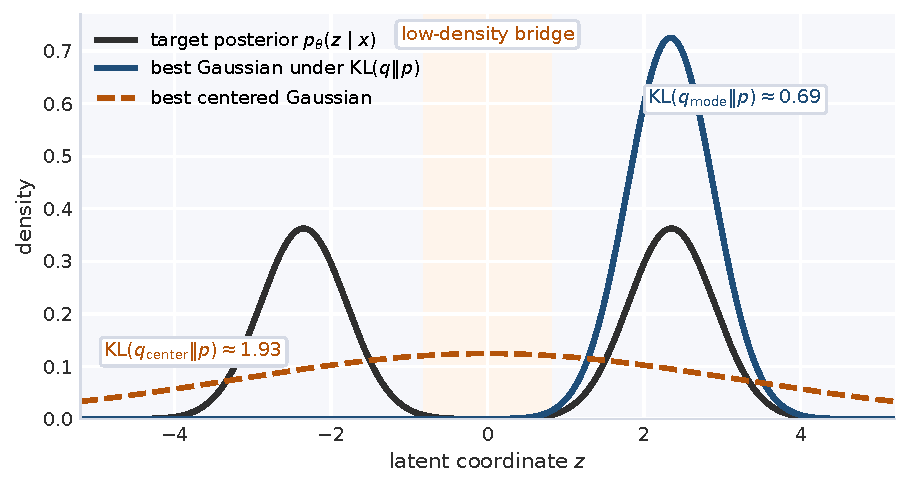
\includegraphics[width=0.92\linewidth]{figures/handouts/elbo_geometry/fig_forward_kl_undercoverage_applied}
  \caption{A bimodal target posterior is approximated by a single Gaussian family.
  The centered Gaussian must place mass in the low-density region between the modes, while the forward-KL minimizer instead concentrates near one mode.
  This is the mode-seeking geometry behind undercoverage.}
  \label{fig:forward-kl-undercoverage-applied}
\end{figure}

In \Cref{fig:forward-kl-undercoverage-applied}, the centered approximation pays for mass throughout the low-density region between the modes, while the forward-KL minimizer avoids that bill and settles on one plausible region.

\begin{exercise}[A three-cell proxy for forward-KL undercoverage]
\label{ex:forward-kl-undercovers}
Approximate a bimodal posterior by three disjoint regions:
\(L\) for the left mode, \(M\) for the low-density middle region, and \(R\) for the right mode.
Suppose
\[
  p(L)=0.49,
  \qquad
  p(M)=0.02,
  \qquad
  p(R)=0.49.
\]
Consider two candidate unimodal approximations:
\[
  q_{\mathrm{mid}}=(0.25,0.50,0.25),
  \qquad
  q_{\mathrm{left}}=(1,0,0),
\]
listed in the order \((L,M,R)\).
\begin{enumerate}[leftmargin=*]
  \item Compute
  \[
    \operatorname{KL}(q_{\mathrm{mid}}\|p)
    =
    \sum_{A\in\{L,M,R\}}
    q_{\mathrm{mid}}(A)\log\frac{q_{\mathrm{mid}}(A)}{p(A)}.
  \]
  \item Compute
  \[
    \operatorname{KL}(q_{\mathrm{left}}\|p).
  \]
  \item Which candidate is preferred by forward KL?
  Explain in one or two sentences which term in the objective makes the centered approximation expensive.
\end{enumerate}
\end{exercise}
\SolutionBox[12]{For the centered candidate,
\[
  \operatorname{KL}(q_{\mathrm{mid}}\|p)
  =
  0.25\log\frac{0.25}{0.49}
  +
  0.50\log\frac{0.50}{0.02}
  +
  0.25\log\frac{0.25}{0.49}
  =
  \frac12\log\frac{625}{49}.
\]
For the left-mode candidate,
\[
  \operatorname{KL}(q_{\mathrm{left}}\|p)
  =
  1\cdot \log\frac{1}{0.49}
  =
  \log\frac{100}{49}.
\]
Numerically,
\[
  \frac12\log\frac{625}{49}\approx 1.27,
  \qquad
  \log\frac{100}{49}\approx 0.71,
\]
so forward KL prefers \(q_{\mathrm{left}}\).
The key penalty is the middle-region term
\[
  0.50\log\frac{0.50}{0.02},
\]
which is large because the centered approximation places substantial mass where the target density is tiny.
This is the discrete version of undercoverage: missing one mode can be cheaper than paying for mass in a low-density middle region.}

The cleanest next example is mean-field VI, where the family deletes dependence before optimization ever starts.

\section{Mean-field deletes dependence before optimization starts}
\label{sec:mean-field-geometry}

\subsection{Factorization is the real approximation}
\label{subsec:mean-field-cavi}

Mean-field VI is the first place where the phrase ``the family is part of the model'' becomes concrete.
Write the latent variable as \(z=(z_1,\dots,z_m)\) and consider the factorized family
\[
  q(z)=\prod_{j=1}^m q_j(z_j).
\]
The point of this choice is not that coordinate ascent is especially deep.
The point is that the posterior is now allowed to move only inside a product geometry.
Any dependence in the true posterior has already been deleted before the optimizer gets to work.

\begin{proposition}[Mean-field coordinate update]
\label{prop:mean-field-update-handout}
Fix all factors except \(q_j\), and assume
\[
  m_j(z_j)\coloneqq \E_{q_{-j}}[\log p_\theta(x,z)]
\]
is finite almost everywhere with \(\int e^{m_j(z_j)}\,dz_j<\infty\).
Then any maximizer of the ELBO over the remaining factor satisfies
\[
  q_j^\star(z_j)
  \propto
  \exp\!\left(
    \E_{q_{-j}}\bigl[\log p_\theta(x,z)\bigr]
  \right),
\]
where the expectation is taken under the current variational law on the remaining coordinates.
\end{proposition}
\begin{proof}
Holding \(q_{-j}\) fixed and optimizing only over \(q_j\), the ELBO becomes
\[
  \mathcal{L}(q;x)
  =
  \int q_j(z_j)\,m_j(z_j)\,dz_j
  -
  \int q_j(z_j)\log q_j(z_j)\,dz_j
  + C,
\]
where \(C\) does not depend on \(q_j\).
Define
\[
  Z_j\coloneqq \int e^{m_j(u)}\,du,
  \qquad
  \widetilde q_j(z_j)\coloneqq Z_j^{-1}e^{m_j(z_j)}.
\]
Then
\[
  \mathcal{L}(q;x)
  =
  -\operatorname{KL}\!\bigl(q_j\,\|\,\widetilde q_j\bigr)+\log Z_j+C,
\]
so the ELBO is maximized at \(q_j=\widetilde q_j\).%
\end{proof}

This is the deterministic analogue of a Gibbs update:
instead of sampling one coordinate from an exact conditional, we replace one factor by the best ELBO fit given the others.
But the more important point is geometric.
Once the family has been factorized, CAVI can only repair the posterior inside that factorized geometry.

\begin{figure}[t]
  \centering
  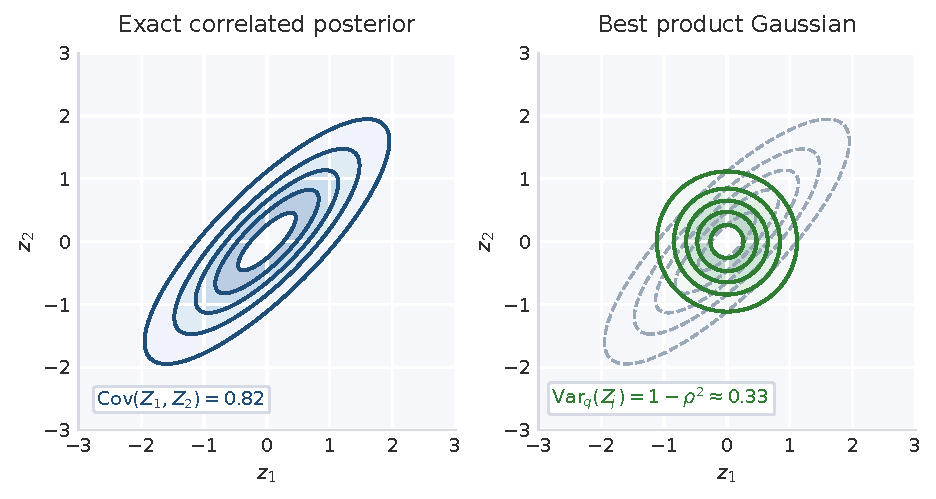
\includegraphics[width=0.92\linewidth]{figures/handouts/elbo_geometry/fig_mean_field_correlation_loss_applied}
  \caption{A correlated Gaussian posterior is compared with the best product Gaussian from the mean-field family.
  The surrogate removes the tilted covariance structure and shrinks each marginal variance, matching the analytic minimizer computed below.}
  \label{fig:mean-field-correlation-loss}
\end{figure}

That loss of geometry is not a training accident.
It is the structural cost of replacing a joint posterior by a product family.
\Cref{fig:mean-field-correlation-loss} shows the cleanest case:
the target posterior is as friendly as possible, but the family is not allowed to tilt.

\begin{proposition}[Best product-Gaussian fit to a correlated Gaussian]
\label{prop:mfvi-gaussian-underdispersion}
Let the exact posterior be
\[
  p_\theta(z\mid x)=\mathcal{N}(0,\Sigma_\rho),
  \qquad
  \Sigma_\rho=
  \begin{bmatrix}
    1 & \rho\\
    \rho & 1
  \end{bmatrix},
  \qquad
  0<|\rho|<1.
\]
Among all fully factorized Gaussian approximations
\[
  q(z_1,z_2)=\mathcal{N}(m_1,s_1^2)\,\mathcal{N}(m_2,s_2^2),
\]
the unique minimizer of
\(\operatorname{KL}(q(z_1,z_2)\|p_\theta(z\mid x))\) satisfies
\[
  m_1=m_2=0,
  \qquad
  s_1^2=s_2^2=1-\rho^2.
\]
In particular, the optimal mean-field approximation is not only uncorrelated; it is also under-dispersed in each coordinate whenever \(\rho\neq 0\).
\end{proposition}
\begin{proof}
The precision matrix is
\[
  \Sigma_\rho^{-1}
  =
  \frac{1}{1-\rho^2}
  \begin{bmatrix}
    1 & -\rho\\
    -\rho & 1
  \end{bmatrix}.
\]
A direct Gaussian-KL calculation gives
\[
  \operatorname{KL}(q\|p_\theta(\cdot\mid x))
  =
  \frac12\left[
    \frac{m_1^2-2\rho m_1m_2+m_2^2+s_1^2+s_2^2}{1-\rho^2}
    -2
    +
    \log\!\frac{1-\rho^2}{s_1^2s_2^2}
  \right].
\]
The quadratic form in \((m_1,m_2)\) is minimized uniquely at \(m_1=m_2=0\).
For \(j\in\{1,2\}\),
\[
  \frac{\partial}{\partial s_j^2}\operatorname{KL}(q\|p_\theta(\cdot\mid x))
  =
  \frac12\left(\frac{1}{1-\rho^2}-\frac{1}{s_j^2}\right),
\]
so the unique stationary point is \(s_j^2=1-\rho^2\).
Since the second derivative with respect to \(s_j^2\) is \(1/(2s_j^4)>0\), this stationary point is the global minimizer.%
\end{proof}

This calculation says exactly what the picture suggests.
The best product approximation cannot reproduce the tilted covariance geometry, so it compensates by shrinking the marginal variances.
Even in the Gaussian case, forward KL plus factorization produces an axis-aligned, overconfident surrogate.

\begin{exercise}[Recover the best product Gaussian]
\label{ex:mean-field-removes-dependence}
Use the displayed formula
\[
  \operatorname{KL}(q\|p_\theta(\cdot\mid x))
  =
  \frac12\left[
    \frac{m_1^2-2\rho m_1m_2+m_2^2+s_1^2+s_2^2}{1-\rho^2}
    -2
    +
    \log\!\frac{1-\rho^2}{s_1^2s_2^2}
  \right]
\]
for the factorized Gaussian \(q(z)=\mathcal{N}(m_1,s_1^2)\mathcal{N}(m_2,s_2^2)\).
\begin{enumerate}[leftmargin=*]
  \item Holding \(s_1^2,s_2^2\) fixed, differentiate with respect to \(m_1,m_2\) and show that the unique stationary point is \(m_1=m_2=0\).
  \item Differentiate with respect to \(s_1^2\) and \(s_2^2\) and show that the minimizer satisfies
  \[
    s_1^2=s_2^2=1-\rho^2.
  \]
  \item Compare these values with the exact posterior variances and covariance. What two geometric distortions does the best product approximation impose?
\end{enumerate}
\end{exercise}
\SolutionBox[12]{Differentiating the KL with respect to the means gives
\[
  \frac{\partial}{\partial m_1}\operatorname{KL}(q\|p_\theta(\cdot\mid x))
  =
  \frac{m_1-\rho m_2}{1-\rho^2},
  \qquad
  \frac{\partial}{\partial m_2}\operatorname{KL}(q\|p_\theta(\cdot\mid x))
  =
  \frac{m_2-\rho m_1}{1-\rho^2}.
\]
The stationary conditions are
\[
  m_1=\rho m_2,
  \qquad
  m_2=\rho m_1.
\]
Since \(|\rho|<1\), the unique solution is \(m_1=m_2=0\).
For the variances,
\[
  \frac{\partial}{\partial s_j^2}\operatorname{KL}(q\|p_\theta(\cdot\mid x))
  =
  \frac12\left(\frac{1}{1-\rho^2}-\frac{1}{s_j^2}\right),
  \qquad j\in\{1,2\},
\]
so the stationary point is \(s_1^2=s_2^2=1-\rho^2\), which is the minimizer.
The exact posterior has marginal variances \(1\) and covariance \(\rho\), while the best product approximation has variances \(1-\rho^2<1\) and covariance \(0\).
So mean-field imposes two distortions at once: it deletes posterior dependence and it shrinks each marginal variance below the true one.}

Up to this point every failure has been local:
one observation, one posterior, one restricted family.
Amortization adds a second restriction across data.

\section{Shared encoders and one latent bottleneck}
\label{sec:shared-encoder-bottleneck}

\subsection{Amortization adds a second restriction}
\label{subsec:amortization-gap}

Amortized VI replaces per-datum variational optimization by a shared encoder \(q_\phi(z\mid x)\).
That makes inference scalable, but it also means that all posterior approximations must lie on the image of one learned map \(x\mapsto q_\phi(\cdot\mid x)\).
On a data set \(x_1,\dots,x_n\), the optimization problem becomes
\[
  \max_{\phi\in\Phi}\sum_{i=1}^n \mathcal{L}(q_\phi(\cdot\mid x_i);x_i)
  \qquad\text{instead of}\qquad
  \sum_{i=1}^n \max_{q\in\mathcal{Q}} \mathcal{L}(q;x_i).
\]
So amortization is not just a faster optimizer for the same approximation problem.
It is a smaller approximation problem.

\begin{figure}[t]
  \centering
  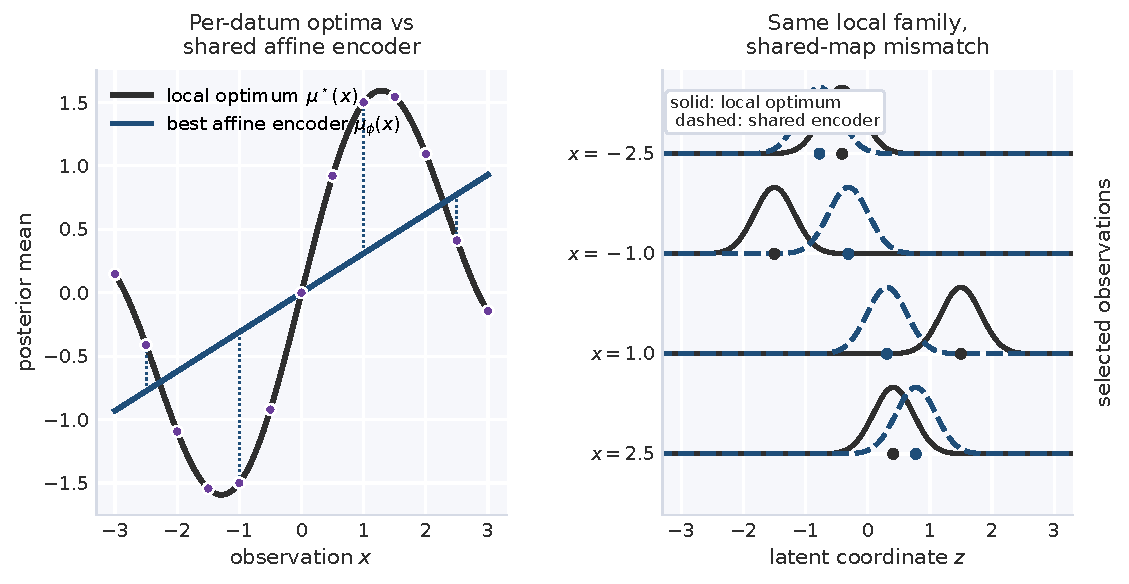
\includegraphics[width=\linewidth]{figures/handouts/elbo_geometry/fig_vi_amortization_applied}
  \caption{A synthetic posterior family with nonlinear per-datum optima \(\mu^\star(x)\) is approximated by a shared affine encoder family.
  The local posteriors are individually representable, but one shared map cannot hit all of the targets simultaneously.
  This is the amortization gap.}
  \label{fig:vi-amortization-handout}
\end{figure}

\Cref{fig:vi-amortization-handout} separates two failure modes that are easy to conflate.
The local family may be adequate for each datum, yet the shared encoder may still miss the local optimum because one map cannot bend in all the required directions at once.

\begin{proposition}[Amortization cannot beat per-datum variational optima]
\label{prop:amortization-gap}
Let \(x_1,\dots,x_n\) be observations, and let \(\mathcal{Q}\) be a variational family available for each datum individually.
Define
\[
  \mathcal{L}_i^\star \coloneqq \sup_{q\in\mathcal{Q}} \mathcal{L}(q;x_i).
\]
Then for any amortized family \(\{q_\phi(\cdot\mid x):\phi\in\Phi\}\subseteq \mathcal{Q}\),
\[
  \sup_{\phi\in\Phi} \sum_{i=1}^n \mathcal{L}(q_\phi(\cdot\mid x_i);x_i)
  \le
  \sum_{i=1}^n \mathcal{L}_i^\star.
\]
\end{proposition}
\begin{proof}
Fix \(\phi\).
For each \(i\), the distribution \(q_\phi(\cdot\mid x_i)\) belongs to \(\mathcal{Q}\), so
\[
  \mathcal{L}(q_\phi(\cdot\mid x_i);x_i)\le \mathcal{L}_i^\star.
\]
Summing over \(i\) gives
\[
  \sum_{i=1}^n \mathcal{L}(q_\phi(\cdot\mid x_i);x_i)\le \sum_{i=1}^n \mathcal{L}_i^\star.
\]
Taking the supremum over \(\phi\) preserves the inequality.%
\end{proof}

The proposition is simple, but it is the correct formal separation between family mismatch and amortization gap.
The gap vanishes only if one shared encoder hits the per-datum optimum everywhere.
Computationally, amortization is still the right idea:
the recognition model and the reparameterized gradient estimator from AEVB and stochastic backpropagation make \(\mathcal{J}(\theta,\phi)\) trainable at scale
\citep[\S\S2.1--2.3]{kingma_welling_2014_aevb}
\citep[\S\S1, 3]{rezende_mohamed_wierstra_2014_stochastic_backpropagation}.
But neither device removes the underlying geometric restriction.

\begin{exercise}[Decompose local mismatch and amortization gap]
\label{ex:amortization-gap}
Let
\[
  \mathcal{L}_i^\star
  \coloneqq
  \sup_{q\in\mathcal{Q}}\mathcal{L}(q;x_i),
  \qquad i=1,\dots,n.
\]
Define the local approximation gap
\[
  \Delta_i^{\mathrm{loc}}
  \coloneqq
  \log p_\theta(x_i)-\mathcal{L}_i^\star
\]
and the amortization gap
\[
  \Delta_{\mathrm{am}}
  \coloneqq
  \sum_{i=1}^n \mathcal{L}_i^\star
  -
  \sup_{\phi\in\Phi}\sum_{i=1}^n \mathcal{L}(q_\phi(\cdot\mid x_i);x_i).
\]
Assume the amortized family satisfies
\[
  \{q_\phi(\cdot\mid x_i):\phi\in\Phi\}\subseteq \mathcal{Q}
  \qquad\text{for every }i.
\]
\begin{enumerate}[leftmargin=*]
  \item Use the ELBO--KL identity to show that, for each \(i\),
  \[
    \Delta_i^{\mathrm{loc}}
    =
    \inf_{q\in\mathcal{Q}}
    \operatorname{KL}\!\bigl(q(z)\,\|\,p_\theta(z\mid x_i)\bigr),
  \]
  and in particular \(\Delta_i^{\mathrm{loc}}\ge 0\).
  \item Use \Cref{prop:amortization-gap} to show \(\Delta_{\mathrm{am}}\ge 0\).
  \item Fix \(\phi\). Show that for each \(i\),
  \[
    \mathcal{L}(q_\phi(\cdot\mid x_i);x_i)\le \mathcal{L}_i^\star.
  \]
  Then sum over \(i\) and take the supremum over \(\phi\) to recover the inequality
  \[
    \sup_{\phi\in\Phi}\sum_{i=1}^n \mathcal{L}(q_\phi(\cdot\mid x_i);x_i)
    \le
    \sum_{i=1}^n \mathcal{L}_i^\star.
  \]
  \item Prove the exact decomposition
  \[
    \sum_{i=1}^n \log p_\theta(x_i)
    -
    \sup_{\phi\in\Phi}\sum_{i=1}^n \mathcal{L}(q_\phi(\cdot\mid x_i);x_i)
    =
    \sum_{i=1}^n \Delta_i^{\mathrm{loc}}
    +
    \Delta_{\mathrm{am}}.
  \]
  \item Explain what vanishes in the two extreme cases:
  a purely local-family-limited regime and a purely amortization-limited regime.
\end{enumerate}
\end{exercise}
\SolutionBox[15]{By the ELBO--KL identity,
\[
  \log p_\theta(x_i)
  =
  \mathcal{L}(q;x_i)
  +
  \operatorname{KL}\!\bigl(q(z)\,\|\,p_\theta(z\mid x_i)\bigr)
\]
for every admissible \(q\in\mathcal{Q}\).
Taking the supremum over \(q\in\mathcal{Q}\) on the ELBO side is the same as taking the infimum of the KL term, so
\[
  \Delta_i^{\mathrm{loc}}
  =
  \log p_\theta(x_i)-\mathcal{L}_i^\star
  =
  \inf_{q\in\mathcal{Q}}
  \operatorname{KL}\!\bigl(q(z)\,\|\,p_\theta(z\mid x_i)\bigr)\ge 0.
\]
Next,
\[
  \Delta_{\mathrm{am}}
  =
  \sum_{i=1}^n \mathcal{L}_i^\star
  -
  \sup_{\phi\in\Phi}\sum_{i=1}^n \mathcal{L}(q_\phi(\cdot\mid x_i);x_i)\ge 0
\]
by \Cref{prop:amortization-gap}.
Fix \(\phi\).
For each datum \(x_i\), the distribution \(q_\phi(\cdot\mid x_i)\) belongs to \(\mathcal{Q}\), so by definition of \(\mathcal{L}_i^\star\),
\[
  \mathcal{L}(q_\phi(\cdot\mid x_i);x_i)\le \mathcal{L}_i^\star.
\]
Summing over \(i\) gives
\[
  \sum_{i=1}^n \mathcal{L}(q_\phi(\cdot\mid x_i);x_i)
  \le
  \sum_{i=1}^n \mathcal{L}_i^\star.
\]
Taking the supremum over \(\phi\) preserves the inequality and yields the claim.
For the exact decomposition, add and subtract \(\sum_i \mathcal{L}_i^\star\):
\begin{align*}
  \sum_{i=1}^n \log p_\theta(x_i)
  -
  \sup_{\phi}\sum_{i=1}^n \mathcal{L}(q_\phi(\cdot\mid x_i);x_i)
  &=
  \sum_{i=1}^n \bigl(\log p_\theta(x_i)-\mathcal{L}_i^\star\bigr) \\
  &\quad
  +
  \sum_{i=1}^n \mathcal{L}_i^\star
  -
  \sup_{\phi}\sum_{i=1}^n \mathcal{L}(q_\phi(\cdot\mid x_i);x_i) \\
  &=
  \sum_{i=1}^n \Delta_i^{\mathrm{loc}}+\Delta_{\mathrm{am}}.
\end{align*}
In a purely local-family-limited regime, \(\Delta_{\mathrm{am}}=0\) and the whole gap comes from the local family \(\mathcal{Q}\) being too small.
In a purely amortization-limited regime, every \(\Delta_i^{\mathrm{loc}}=0\) and the whole gap comes from one shared encoder failing to realize the per-datum optima.}

\subsection{Blur: overlapping latent neighborhoods force averaging}
\label{subsec:blur}

From this point on, keep the standard one-bottleneck VAE in mind:
a prior \(p(z)\), decoder \(p_\theta(x\mid z)\), and shared encoder \(q_\phi(z\mid x)\).
This is the AEVB setting with the usual reparameterization
\[
  z=\mu_\phi(x)+\sigma_\phi(x)\odot \varepsilon,
  \qquad
  \varepsilon\sim\mathcal{N}(0,I),
\]
which makes stochastic ELBO optimization practical but does not alter the geometry of the approximation problem
\citep[\S\S2.1--2.3]{kingma_welling_2014_aevb}
\citep[\S3]{rezende_mohamed_wierstra_2014_stochastic_backpropagation}.

The blur mechanism becomes sharp when the decoder is Gaussian.
Then, for fixed \(q_\phi\), decoder learning is literally a regression problem under the joint law induced by the data and the encoder.
That is the direct link from ``posterior overlap'' to blurry reconstructions.

\begin{proposition}[A fixed-encoder Gaussian VAE is regression under \(p_{\mathrm{data}}(x)q_\phi(z\mid x)\)]
\label{prop:gaussian-vae-regression}
Assume \(\sigma^2>0\) is fixed and
\[
  p_\theta(x\mid z)=\mathcal{N}\!\bigl(\mu_\theta(z),\sigma^2 I\bigr).
\]
Then the expected ELBO over the data distribution satisfies
\[
  \E_{p_{\mathrm{data}}(x)}\!\bigl[\mathcal{L}(q_\phi;x)\bigr]
  =
  C(\phi,\sigma^2)
  -
  \frac{1}{2\sigma^2}
  \E_{(X,Z)\sim \pi_\phi}\!\bigl[\norm{X-\mu_\theta(Z)}_2^2\bigr],
\]
where
\[
  \pi_\phi(dx,dz)\coloneqq p_{\mathrm{data}}(x)\,q_\phi(dz\mid x)
\]
and
\[
  C(\phi,\sigma^2)
  =
  -\frac{d}{2}\log(2\pi\sigma^2)
  -
  \E_{p_{\mathrm{data}}(x)}
  \operatorname{KL}\!\bigl(q_\phi(z\mid x)\,\|\,p(z)\bigr)
\]
does not depend on \(\mu_\theta\).
Consequently, for fixed \(q_\phi\), maximizing the expected ELBO over decoder means \(\mu_\theta\) is equivalent to minimizing
\[
  \mu\mapsto
  \E_{(X,Z)\sim \pi_\phi}\!\bigl[\norm{X-\mu(Z)}_2^2\bigr].
\]
\end{proposition}
\begin{proof}
For each \(x\),
\[
  \mathcal{L}(q_\phi;x)
  =
  \E_{q_\phi(z\mid x)}[\log p_\theta(x\mid z)]
  -
  \operatorname{KL}\!\bigl(q_\phi(z\mid x)\,\|\,p(z)\bigr).
\]
Under the Gaussian decoder,
\[
  \log p_\theta(x\mid z)
  =
  -\frac{d}{2}\log(2\pi\sigma^2)
  -
  \frac{1}{2\sigma^2}\norm{x-\mu_\theta(z)}_2^2.
\]
Taking expectations over \(p_{\mathrm{data}}(x)\) gives
\begin{align*}
  \E_{p_{\mathrm{data}}(x)}\!\bigl[\mathcal{L}(q_\phi;x)\bigr]
  &=
  -\frac{d}{2}\log(2\pi\sigma^2)
  -
  \frac{1}{2\sigma^2}
  \E_{p_{\mathrm{data}}(x)q_\phi(z\mid x)}
  \norm{x-\mu_\theta(z)}_2^2 \\
  &\quad
  -
  \E_{p_{\mathrm{data}}(x)}
  \operatorname{KL}\!\bigl(q_\phi(z\mid x)\,\|\,p(z)\bigr),
\end{align*}
which is the stated identity.%
\end{proof}

\begin{proposition}[Squared loss chooses conditional means]
\label{prop:squared-error-mean}
Let \((X,Z)\) be jointly distributed with \(X\in\R^d\), \(Z\in\R^m\), and \(\E\norm{X}_2^2<\infty\).
Among all measurable maps \(\mu:\R^m\to\R^d\) such that \(\E\norm{\mu(Z)}_2^2<\infty\), the minimizer of
\[
  \mu\mapsto \E\norm{X-\mu(Z)}_2^2
\]
satisfies
\[
  \mu^\star(Z)=\E[X\mid Z]
\]
almost surely, where \(\E[X\mid Z]\) denotes any version of the conditional expectation.
\end{proposition}
\begin{proof}
For any measurable \(\mu\),
\begin{align*}
  \E\norm{X-\mu(Z)}_2^2
  &=
  \E\norm{X-\E[X\mid Z]}_2^2
  +
  \E\norm{\E[X\mid Z]-\mu(Z)}_2^2 \\
  &\quad
  +
  2\,\E\!\left[
    \ip{X-\E[X\mid Z]}{\E[X\mid Z]-\mu(Z)}
  \right].
\end{align*}
The cross term vanishes because
\[
  \E\!\left[X-\E[X\mid Z]\mid Z\right]=0
\]
and \(\E[X\mid Z]-\mu(Z)\) is \(Z\)-measurable.
Therefore
\[
  \E\norm{X-\mu(Z)}_2^2
  =
  \E\norm{X-\E[X\mid Z]}_2^2
  +
  \E\norm{\E[X\mid Z]-\mu(Z)}_2^2,
\]
so the minimum is attained exactly when \(\mu(Z)=\E[X\mid Z]\) almost surely.%
\end{proof}

\Cref{prop:gaussian-vae-regression} and \Cref{prop:squared-error-mean} give the blur mechanism in one line:
for fixed \(q_\phi\), a Gaussian decoder mean that minimizes the reconstruction risk is any version of
\[
  \mu_\theta^\star(Z)=\E_{\pi_\phi}[X\mid Z]
\]
almost surely.
So if the encoder geometry pushes several incompatible observations into the same latent neighborhood, the decoder is forced toward a conditional mean rather than any one sharp sample.
This makes precise the ``posterior overlap'' and ``locality'' story emphasized in the \(\beta\)-VAE discussion of \citet[\S\S4.2--5]{burgess_higgins_pal_matthey_watters_desjardins_lerchner_2018_understanding_bvae}.

\subsubsection{A two-point blur example}
\label{subsubsec:two-point-blur}

The abstract conditional-mean statement becomes concrete in the smallest nontrivial example.
If one latent neighborhood mixes two genuinely different observations, the decoder has no sharper target available than their average.

\begin{example}[Ambiguity forces averaging]
\label{ex:two-point-blur}
Suppose the data distribution places probability \(1/2\) on \(x^{(1)}\in\R^d\) and probability \(1/2\) on \(x^{(2)}\in\R^d\), and suppose that a version of the conditional law of \(X\) given \(Z\) satisfies, at some latent location \(z\),
\[
  \Pr(X=x^{(1)}\mid Z=z)
  =
  \Pr(X=x^{(2)}\mid Z=z)
  =
  \frac12.
\]
Then a risk-minimizing Gaussian-decoder prediction at that latent point is
\[
  \mu_\theta(z)
  =
  \E[X\mid Z=z]
  =
  \frac{x^{(1)}+x^{(2)}}{2}.
\]
Unless \(x^{(1)}=x^{(2)}\), the reconstruction is an average rather than an actual datum.
\end{example}

The example is tiny, but it captures the full story.
Blur does not mean the decoder is inherently bad at detail.
It means the encoder geometry failed to separate distinctions that matter to squared-error reconstruction.
When the bottleneck has too little effective capacity, the decoder is rewarded for averaging unresolved variation
\citep[\S\S4.2--5]{burgess_higgins_pal_matthey_watters_desjardins_lerchner_2018_understanding_bvae}.

\begin{figure}[t]
  \centering
  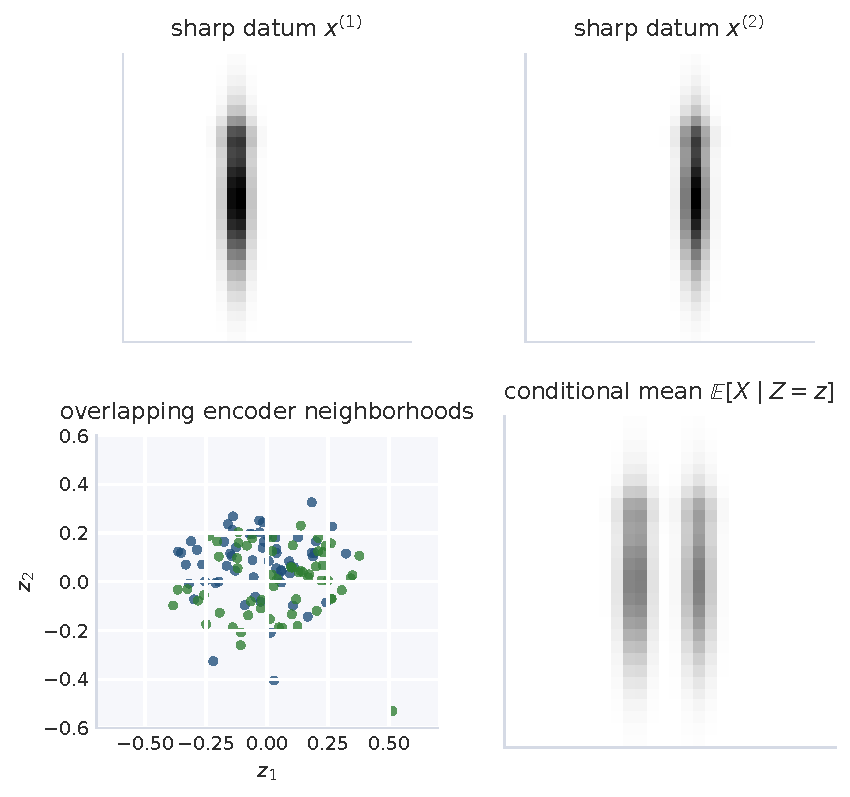
\includegraphics[width=0.84\linewidth]{figures/handouts/elbo_geometry/fig_latent_overlap_blur_applied}
  \caption{Two distinct sharp observations are mapped into nearly the same latent neighborhood.
  A Gaussian decoder therefore returns their conditional mean, which is visibly blurrier than either endpoint.}
  \label{fig:latent-overlap-blur}
\end{figure}

\begin{exercise}[The irreducible blur penalty]
\label{ex:blur-average}
In the two-point example above, show the exact identity
\[
  \frac12\norm{x^{(1)}-a}_2^2+\frac12\norm{x^{(2)}-a}_2^2
  =
  \frac14\norm{x^{(1)}-x^{(2)}}_2^2
  +
  \norm{a-\tfrac12(x^{(1)}+x^{(2)})}_2^2.
\]
Deduce that the minimizer is \(a=(x^{(1)}+x^{(2)})/2\) and compute the minimum value explicitly in terms of \(\norm{x^{(1)}-x^{(2)}}_2\).
Then explain how this finite identity mirrors the decomposition in \Cref{prop:squared-error-mean}.
\end{exercise}
\SolutionBox[9]{Expanding the quadratic gives
\[
  \frac12\norm{x^{(1)}-a}_2^2+\frac12\norm{x^{(2)}-a}_2^2
  =
  \frac14\norm{x^{(1)}-x^{(2)}}_2^2
  +
  \norm{a-\tfrac12(x^{(1)}+x^{(2)})}_2^2.
\]
Hence the minimizer is the midpoint \(a=(x^{(1)}+x^{(2)})/2\).
The minimum value is
\[
  \frac14\norm{x^{(1)}-x^{(2)}}_2^2.
\]
This is the two-point version of \Cref{prop:squared-error-mean}: the first term is the irreducible conditional-variance cost, and the second term is the extra penalty for choosing a prediction different from the conditional mean.
So even the best decoder incurs a positive reconstruction penalty whenever distinct observations share one latent code.}

\subsection{Collapse: the decoder can make latent information too expensive}
\label{subsec:collapse}

Blur and collapse are opposite-looking symptoms of the same bottleneck picture.
In blur, the latent code is used but is not expressive enough to separate incompatible observations.
In collapse, the decoder becomes so strong that using \(z\) is not worth the KL bill.
The cleanest formal toy case is when the decoder literally ignores \(z\).

\begin{proposition}[If the decoder ignores \(z\), the ELBO prefers the prior]
\label{prop:collapse-if-decoder-ignores-z}
Suppose \(p_\theta(x\mid z)=p_\theta(x)\) for all \(z\).
Then for every \(x\),
\[
  \mathcal{L}(q;x)=\log p_\theta(x)-\operatorname{KL}\!\bigl(q(z)\,\|\,p(z)\bigr),
\]
so the ELBO is maximized by \(q(z)=p(z)\).
\end{proposition}
\begin{proof}
Under the assumption \(p_\theta(x\mid z)=p_\theta(x)\),
\[
  p_\theta(x,z)=p_\theta(x)\,p(z).
\]
Substituting this into the ELBO gives
\[
  \mathcal{L}(q;x)
  =
  \E_q[\log p_\theta(x)+\log p(z)-\log q(z)]
  =
  \log p_\theta(x)-\operatorname{KL}\!\bigl(q(z)\,\|\,p(z)\bigr).
\]
The KL term is minimized at \(q(z)=p(z)\), proving the claim.%
\end{proof}

Real posterior collapse is usually less extreme than this toy case, but the geometry is the same.
If the decoder can already explain \(x\) well enough on its own, then the ELBO charges for transmitting information through \(z\) without demanding much in return.
The latent variable becomes expendable.

To see the bill more clearly, average the KL term over the data distribution and define the aggregate posterior
\[
  q_\phi(z)
  \coloneqq
  \int q_\phi(z\mid x)\,p_{\mathrm{data}}(x)\,dx.
\]

\begin{proposition}[Mutual-information decomposition of the KL term]
\label{prop:mi-decomposition}
Assume \(q_\phi(z\mid x)\) and \(p(z)\) are densities with respect to a common base measure and that the displayed expectations are finite.
We have
\[
  \E_{p_{\mathrm{data}}(x)}
  \operatorname{KL}\!\bigl(q_\phi(z\mid x)\,\|\,p(z)\bigr)
  =
  I_q(X;Z)
  +
  \operatorname{KL}\!\bigl(q_\phi(z)\,\|\,p(z)\bigr),
\]
where \(I_q(X;Z)\) is mutual information under the joint law
\[
  p_{\mathrm{data}}(x)\,q_\phi(z\mid x).
\]
\end{proposition}
\begin{proof}
Expand the left-hand side:
\[
  \E_{p_{\mathrm{data}}(x)q_\phi(z\mid x)}
  \bigl[\log q_\phi(z\mid x)-\log p(z)\bigr].
\]
Add and subtract \(\log q_\phi(z)\):
\[
  \E\!\bigl[\log q_\phi(z\mid x)-\log q_\phi(z)\bigr]
  +
  \E\!\bigl[\log q_\phi(z)-\log p(z)\bigr].
\]
The first term is \(I_q(X;Z)\), and the second is
\(\operatorname{KL}(q_\phi(z)\|p(z))\).%
\end{proof}

Combining \Cref{prop:mi-decomposition} with the expected ELBO gives
\[
  \E_{p_{\mathrm{data}}(x)}\!\bigl[\mathcal{L}(q_\phi;x)\bigr]
  =
  \E_{p_{\mathrm{data}}(x)q_\phi(z\mid x)}[\log p_\theta(x\mid z)]
  -
  I_q(X;Z)
  -
  \operatorname{KL}\!\bigl(q_\phi(z)\,\|\,p(z)\bigr).
\]
So the KL regularizer is charging for two things at once:
how much information the code stores about the data, and how far the aggregate code distribution drifts from the prior.
If the decoder class already contains good nearly unconditional models for the data, the collapsed solution can be globally competitive; more generally, using \(z\) is worthwhile only when the reconstruction gain beats this information bill.

This helps explain why expressive autoregressive decoders often collapse in practice.
Bowman et al.\ show the sentence-VAE version of this story:
if the decoder is already a strong language model, training pushes \(q_\phi(z\mid x)\) back toward the prior unless the optimization pressure is modified
\citep[\S3.1]{bowman_vilnis_vinyals_dai_jozefowicz_bengio_2016_generating_sentences}.
He et al.\ give the complementary dynamic explanation:
early in training the decoder can move faster than the inference network, and that lag can steer the system into a collapsed regime before the encoder learns to use \(z\)
\citep[\S\S3--4]{he_spokoyny_neubig_bergkirkpatrick_2019_lagging_inference}.

\begin{figure}[t]
  \centering
  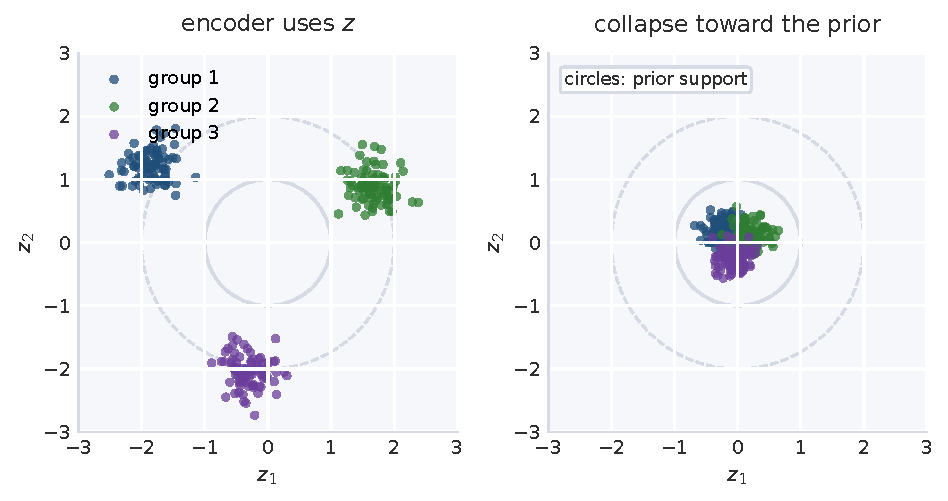
\includegraphics[width=0.90\linewidth]{figures/handouts/elbo_geometry/fig_decoder_bypass_collapse_applied}
  \caption{Toy encoder outputs for three groups of observations.
  When the latent variable is used, the group-conditioned posteriors separate in latent space; under posterior collapse they contract back toward the prior and overlap heavily, so little information about \(x\) remains in \(z\).}
  \label{fig:decoder-bypass-collapse}
\end{figure}

This also clarifies what KL warm-up and \(\beta\)-VAE style heuristics do.
They change the price of information.
That can change which local optimum training reaches, but it does not enlarge the variational family or remove the possibility of collapse
\citep[\S3.1]{bowman_vilnis_vinyals_dai_jozefowicz_bengio_2016_generating_sentences}
\citep[\S\S3--5]{burgess_higgins_pal_matthey_watters_desjardins_lerchner_2018_understanding_bvae}.

\begin{exercise}[\(\beta\)-ELBO as a weighted information budget]
\label{ex:beta-elbo}
Consider the \(\beta\)-ELBO
\[
  \mathcal{L}_\beta(q;x)
  =
  \E_q[\log p_\theta(x\mid z)]
  -
  \beta\,\operatorname{KL}\!\bigl(q(z)\,\|\,p(z)\bigr).
\]
\begin{enumerate}[leftmargin=*]
  \item After averaging over \(p_{\mathrm{data}}(x)\), write the objective as
  \[
    \E_{p_{\mathrm{data}}(x)q_\phi(z\mid x)}[\log p_\theta(x\mid z)]
    -
    \beta\,\E_{p_{\mathrm{data}}(x)}
    \operatorname{KL}\!\bigl(q_\phi(z\mid x)\,\|\,p(z)\bigr).
  \]
  \item In the averaged KL term, add and subtract \(\log q_\phi(z)\) exactly as in the proof of \Cref{prop:mi-decomposition}.
  \item Identify the two resulting terms and conclude that
  \[
    \E_{p_{\mathrm{data}}(x)}[\mathcal{L}_\beta(q_\phi;x)]
    =
    \E_{p_{\mathrm{data}}(x)q_\phi(z\mid x)}[\log p_\theta(x\mid z)]
    -
    \beta\,I_q(X;Z)
    -
    \beta\,\operatorname{KL}\!\bigl(q_\phi(z)\,\|\,p(z)\bigr).
  \]
  \item State separately what large \(\beta\) and small \(\beta\) do to the two non-reconstruction terms.
\end{enumerate}
\end{exercise}
\SolutionBox[10]{Apply \Cref{prop:mi-decomposition} to the averaged KL term:
\[
  \E_{p_{\mathrm{data}}(x)}
  \operatorname{KL}\!\bigl(q_\phi(z\mid x)\,\|\,p(z)\bigr)
  =
  I_q(X;Z)
  +
  \operatorname{KL}\!\bigl(q_\phi(z)\,\|\,p(z)\bigr).
\]
More explicitly,
\[
  \E\!\bigl[\log q_\phi(z\mid x)-\log p(z)\bigr]
  =
  \E\!\bigl[\log q_\phi(z\mid x)-\log q_\phi(z)\bigr]
  +
  \E\!\bigl[\log q_\phi(z)-\log p(z)\bigr],
\]
where the first expectation is \(I_q(X;Z)\) and the second is
\(\operatorname{KL}(q_\phi(z)\|p(z))\).
Substituting into the expected \(\beta\)-ELBO yields
\[
  \E_{p_{\mathrm{data}}(x)}[\mathcal{L}_\beta(q_\phi;x)]
  =
  \E_{p_{\mathrm{data}}(x)q_\phi(z\mid x)}[\log p_\theta(x\mid z)]
  -
  \beta\,I_q(X;Z)
  -
  \beta\,\operatorname{KL}\!\bigl(q_\phi(z)\,\|\,p(z)\bigr).
\]
So \(\beta\) directly rescales both parts of the KL bill.
Large \(\beta\) makes informative codes and prior mismatch expensive, which pushes toward weaker latent usage and can favor collapse.
Small \(\beta\) relaxes both penalties, so the model is more willing to store information in \(z\) and to let the aggregate posterior drift from the prior.
This changes optimization pressure, but it does not enlarge the family \(q_\phi(z\mid x)\), so it does not remove the underlying geometric mismatch.}

\section{Structural redesigns}
\label{sec:structural-redesigns}

Once the problem is framed this way, the right fix is often not ``optimize the same ELBO harder''.
If one latent layer is too coarse, or if learning the encoder geometry itself is unstable, then the approximation problem must change.
Two recurring redesigns do that:
hierarchy and fixed-bridge latent models.

\subsection{Hierarchy splits one overloaded KL bill into local bills}
\label{subsec:hierarchy-redistributes-kl}

A hierarchical VAE replaces one bottleneck by a stack of latent variables.
The key point is not just that the network is deeper.
The important change is that no single latent variable has to pay for every kind of variation at once.
Coarse structure can be represented high in the hierarchy and local detail lower down, so the ELBO decomposes into several local KL penalties instead of one global bottleneck charge.

Consider a hierarchical VAE with latent variables \(z_{1:L}\) and factorization
\[
  p_\theta(x,z_{1:L})
  =
  p_\theta(x\mid z_1)\,
  \prod_{\ell=1}^{L-1} p_\theta(z_\ell\mid z_{\ell+1})\,
  p(z_L),
\]
together with a structured encoder
\[
  q_\phi(z_{1:L}\mid x)
  =
  q_\phi(z_L\mid x)\,
  \prod_{\ell=1}^{L-1} q_\phi(z_\ell\mid z_{\ell+1},x).
\]

\begin{proposition}[Hierarchical ELBO as reconstruction minus local KL terms]
\label{prop:hierarchical-elbo}
For the model and encoder above,
\begin{align*}
  \mathcal{L}(q_\phi;x)
  &=
  \E_{q_\phi}\bigl[\log p_\theta(x\mid z_1)\bigr]
  -
  \operatorname{KL}\!\bigl(q_\phi(z_L\mid x)\,\|\,p(z_L)\bigr) \\
  &\quad
  -
  \sum_{\ell=1}^{L-1}
  \E_{q_\phi(z_{\ell+1:L}\mid x)}\!\left[
    \operatorname{KL}\!\bigl(
      q_\phi(z_\ell\mid z_{\ell+1},x)\,\|\,p_\theta(z_\ell\mid z_{\ell+1})
    \bigr)
  \right].
\end{align*}
\end{proposition}
\begin{proof}
Start from
\[
  \mathcal{L}(q_\phi;x)
  =
  \E_{q_\phi}\!\bigl[\log p_\theta(x,z_{1:L})-\log q_\phi(z_{1:L}\mid x)\bigr].
\]
Substituting the factorizations of \(p_\theta\) and \(q_\phi\) gives
\begin{align*}
  \mathcal{L}(q_\phi;x)
  &=
  \E_{q_\phi}[\log p_\theta(x\mid z_1)] \\
  &\quad
  +
  \E_{q_\phi}\!\left[
    \sum_{\ell=1}^{L-1} \log p_\theta(z_\ell\mid z_{\ell+1})
    + \log p(z_L)
    - \sum_{\ell=1}^{L-1} \log q_\phi(z_\ell\mid z_{\ell+1},x)
    - \log q_\phi(z_L\mid x)
  \right].
\end{align*}
The top-level terms combine as
\[
  \E_{q_\phi}\!\left[\log p(z_L)-\log q_\phi(z_L\mid x)\right]
  =
  -\operatorname{KL}\!\bigl(q_\phi(z_L\mid x)\,\|\,p(z_L)\bigr).
\]
For each \(\ell\in\{1,\dots,L-1\}\),
\begin{align*}
  &\E_{q_\phi}\!\left[
    \log p_\theta(z_\ell\mid z_{\ell+1})
    -
    \log q_\phi(z_\ell\mid z_{\ell+1},x)
  \right] \\
  &\qquad
  =
  -\E_{q_\phi(z_{\ell+1:L}\mid x)}\!\left[
    \operatorname{KL}\!\bigl(
      q_\phi(z_\ell\mid z_{\ell+1},x)\,\|\,p_\theta(z_\ell\mid z_{\ell+1})
    \bigr)
  \right].
\end{align*}
Substituting these identities back into the ELBO gives the result.%
\end{proof}

\Cref{prop:hierarchical-elbo} is the structural point in formula form.
The ELBO no longer contains one global penalty that forces a single latent variable to trade off every kind of information simultaneously.
Instead it contains a top-level prior-matching term and a sum of local conditional KL penalties.
That is why hierarchy can relieve both blur and collapse:
different scales of variation can be distributed across levels rather than compressed through one code.
This is exactly the design philosophy behind deep hierarchical VAEs such as NVAE, where global structure is represented high in the hierarchy and local detail is refined lower down
\citep[\S3.1]{vahdat_kautz_2020_nvae}.

\begin{figure}[t]
  \centering
  \begin{tikzpicture}[>=Stealth,font=\footnotesize]
  \tikzset{
    elbopanel/.style={
      draw=stat221Gray!30,
      fill=white,
      rounded corners=5pt,
      line width=0.6pt
    },
    elbotitle/.style={font=\small\bfseries, text=stat221Gray!90},
    latbox/.style={
      rounded corners=3pt,
      minimum width=1.95cm,
      minimum height=0.76cm,
      line width=0.8pt
    },
    elbobadge/.style={
      rounded corners=2pt,
      inner sep=2.6pt,
      font=\footnotesize,
      align=center,
      text=stat221Gray!85
    }
  }
  \path[use as bounding box] (-0.15,-0.24) rectangle (13.45,5.15);

  \node[elbopanel,minimum width=4.10cm,minimum height=4.95cm,anchor=north west] (leftpanel) at (0.0,4.85) {};
  \node[elbopanel,minimum width=4.10cm,minimum height=4.95cm,anchor=north west] (midpanel) at (4.62,4.85) {};
  \node[elbopanel,minimum width=4.10cm,minimum height=4.95cm,anchor=north west] (rightpanel) at (9.24,4.85) {};

  \node[elbotitle,anchor=north west] at ([xshift=0.25cm,yshift=-0.28cm]leftpanel.north west) {Single bottleneck};
  \node[elbotitle,anchor=north west] at ([xshift=0.25cm,yshift=-0.28cm]midpanel.north west) {Hierarchy splits scales};
  \node[elbotitle,anchor=north west] at ([xshift=0.25cm,yshift=-0.28cm]rightpanel.north west) {Cleaner allocation};

  \node[latbox,draw=stat221Purple!72!black,fill=stat221PurpleLight,minimum width=1.18cm,minimum height=0.68cm] (coarse) at (0.95,3.15) {class};
  \node[latbox,draw=stat221Blue!72!black,fill=stat221BlueLight,minimum width=1.28cm,minimum height=0.68cm] (detail) at (2.05,3.15) {detail};
  \node[latbox,draw=stat221Orange!78!black,fill=stat221OrangeLight,minimum width=1.22cm,minimum height=0.68cm] (noise) at (3.15,3.15) {noise};
  \node[latbox,draw=stat221Purple!72!black,fill=stat221PurpleLight,minimum width=2.15cm,minimum height=0.88cm] (z) at (2.05,1.95) {$z$};
  \node[latbox,draw=stat221Green!68!black,fill=stat221GreenLight,minimum width=2.15cm,minimum height=0.88cm] (x) at (2.05,0.75) {$x$};
  \draw[->,stat221Gray!75,line width=0.85pt] (coarse.south) -- (z.north west);
  \draw[->,stat221Gray!75,line width=0.85pt] (detail.south) -- (z.north);
  \draw[->,stat221Gray!75,line width=0.85pt] (noise.south) -- (z.north east);
  \draw[->,stat221Gray!75,line width=0.85pt] (z) -- (x);
  \node[elbobadge,fill=stat221Gray!8,anchor=west] at (2.72,1.30) {one KL budget};

  \node[latbox,draw=stat221Purple!72!black,fill=stat221PurpleLight,minimum width=2.05cm,minimum height=0.88cm] (z2) at (6.68,3.05) {$z_2$};
  \node[latbox,draw=stat221Blue!72!black,fill=stat221BlueLight,minimum width=2.05cm,minimum height=0.88cm] (z1) at (6.68,1.92) {$z_1$};
  \node[latbox,draw=stat221Green!68!black,fill=stat221GreenLight,minimum width=2.05cm,minimum height=0.88cm] (xh) at (6.68,0.78) {$x$};
  \draw[->,stat221Gray!75,line width=0.85pt] (z2) -- (z1);
  \draw[->,stat221Gray!75,line width=0.85pt] (z1) -- (xh);
  \node[elbobadge,fill=stat221PurpleLight,anchor=east,text=stat221Purple!75!black] at (5.28,3.05) {global};
  \node[elbobadge,fill=stat221BlueLight,anchor=east,text=stat221Blue!75!black] at (5.28,1.92) {local};
  \node[elbobadge,fill=stat221Gray!8,anchor=west] at (7.42,2.47) {$\operatorname{KL}_2$};
  \node[elbobadge,fill=stat221Gray!8,anchor=west] at (7.42,1.34) {$\operatorname{KL}_1$};

  \node[latbox,draw=stat221Purple!72!black,fill=stat221PurpleLight,text width=1.05cm,align=center,inner xsep=2.6pt] (cat1) at (10.31,3.00) {class 1};
  \node[latbox,draw=stat221Purple!72!black,fill=stat221PurpleLight,text width=1.05cm,align=center,inner xsep=2.6pt] (cat2) at (12.26,3.00) {class 2};
  \node[latbox,draw=stat221Blue!72!black,fill=stat221BlueLight,minimum width=0.98cm,minimum height=0.60cm,inner xsep=1.2pt] (d11) at (9.86,1.45) {a};
  \node[latbox,draw=stat221Blue!72!black,fill=stat221BlueLight,minimum width=0.98cm,minimum height=0.60cm,inner xsep=1.2pt] (d12) at (10.81,1.45) {b};
  \node[latbox,draw=stat221Blue!72!black,fill=stat221BlueLight,minimum width=0.98cm,minimum height=0.60cm,inner xsep=1.2pt] (d21) at (11.81,1.45) {a};
  \node[latbox,draw=stat221Blue!72!black,fill=stat221BlueLight,minimum width=0.98cm,minimum height=0.60cm,inner xsep=1.2pt] (d22) at (12.76,1.45) {b};
  \draw[->,stat221Gray!75,line width=0.85pt] (cat1) -- (d11);
  \draw[->,stat221Gray!75,line width=0.85pt] (cat1) -- (d12);
  \draw[->,stat221Gray!75,line width=0.85pt] (cat2) -- (d21);
  \draw[->,stat221Gray!75,line width=0.85pt] (cat2) -- (d22);
  \node[
    elbobadge,
    fill=stat221Gray!8,
    anchor=south,
    text width=3.15cm,
    inner ysep=1.4pt
  ] at ([yshift=0.14cm]rightpanel.south) {coarse choice first,\\local detail second};
\end{tikzpicture}

  \caption{Hierarchy replaces one overloaded bottleneck by several latent levels.
  Coarse structure can be represented high in the hierarchy and local detail low in the hierarchy, so the ELBO splits the information budget across scales instead of forcing one latent code to carry everything.}
  \label{fig:hierarchy-redistributes-kl}
\end{figure}

\subsection{Diffusion prescribes the forward bridge}
\label{subsec:fixed-encoder-geometry}

The diffusion-models unit starts from a chosen bridge between endpoint laws \(p_0\) and \(p_1\), together with a specification of the intermediate path.
In the common reference-noise constructions, reverse-time sampling is then built from endpoint-conditioned bridge steps and the corresponding endpoint posteriors.

For the present handout, the useful comparison comes after time discretization.
Suppose the learned reverse model factors as
\[
  p_\theta(x,z_{1:T})
  =
  p_\theta(x\mid z_1)\,
  \prod_{t=2}^T p_\theta(z_{t-1}\mid z_t)\,
  p(z_T),
\]
and the prescribed forward bridge is written backward as
\[
  q_{\mathrm{fwd}}(z_{1:T}\mid x)
  =
  q_{\mathrm{fwd}}(z_T\mid x)\,
  \prod_{t=2}^T q_{\mathrm{fwd}}(z_{t-1}\mid z_t,x).
\]
Applying the ELBO identity to this latent-variable model gives
\begin{align*}
  \mathcal{L}_{\mathrm{diff}}(\theta;x)
  &=
  \E_{q_{\mathrm{fwd}}(z_{1:T}\mid x)}[\log p_\theta(x\mid z_1)]
  -
  \operatorname{KL}\!\bigl(q_{\mathrm{fwd}}(z_T\mid x)\,\|\,p(z_T)\bigr) \\
  &\quad
  -
  \sum_{t=2}^T
  \E_{q_{\mathrm{fwd}}(z_{t:T}\mid x)}\!\left[
    \operatorname{KL}\!\bigl(q_{\mathrm{fwd}}(z_{t-1}\mid z_t,x)\,\|\,p_\theta(z_{t-1}\mid z_t)\bigr)
    \right].
\end{align*}
This is the same local-KL pattern as the hierarchical VAE:
one reconstruction term, one terminal prior-matching term, and one local conditional KL for each intermediate transition.
What changes is the source of the encoder-side geometry:
the forward chain is prescribed in advance rather than learned from data.
In that precise sense, the continuous-time story in the diffusion-models unit is bridge-first, and the ELBO appears only after the bridge is discretized.

That is the right lineage to remember:
\[
  \text{one-bottleneck VAE}
  \;\longrightarrow\;
  \text{hierarchical VAE}
  \;\longrightarrow\;
  \text{fixed-bridge latent model}.
\]
Viewed variationally, the bookkeeping stays recognizable while the forward bridge is frozen
\citep[Thm.~2.2.3 and the remark on p.~52]{lai_song_kim_mitsufuji_ermon_2025_principles_diffusion}
\citep[\S\S3--4]{kingma_salimans_poole_ho_2021_variational_diffusion}.

\begin{exercise}[Compare hierarchical and fixed-bridge ELBOs]
\label{ex:hierarchy-fixed-encoder}
Specialize \Cref{prop:hierarchical-elbo} to three latent levels \(z_1,z_2,z_3\).
Start from
\[
  \mathcal{L}(q_\phi;x)
  =
  \E_{q_\phi}\!\bigl[\log p_\theta(x,z_{1:3})-\log q_\phi(z_{1:3}\mid x)\bigr]
\]
and the factorizations
\[
  p_\theta(x,z_{1:3})
  =
  p_\theta(x\mid z_1)\,p_\theta(z_1\mid z_2)\,p_\theta(z_2\mid z_3)\,p(z_3),
\]
\[
  q_\phi(z_{1:3}\mid x)
  =
  q_\phi(z_3\mid x)\,q_\phi(z_2\mid z_3,x)\,q_\phi(z_1\mid z_2,x).
\]
\begin{enumerate}[leftmargin=*]
  \item Expand \(\log p_\theta(x,z_{1:3})-\log q_\phi(z_{1:3}\mid x)\) into one reconstruction term, three model terms, and three encoder terms.
  \item Group the \(z_3\) terms into one top-level KL term and the remaining pairs into two expected conditional KL terms.
  \item Compare your expression with the fixed-bridge ELBO in the diffusion subsection and match the terms one by one.
  \item In the hierarchical VAE, which \(q\)-objects are learned?
  In the fixed-bridge diffusion model, which \(q_{\mathrm{fwd}}\)-objects are prescribed instead?
\end{enumerate}
\end{exercise}
\SolutionBox[14]{Expanding the ELBO gives
\begin{align*}
  \mathcal{L}(q_\phi;x)
  &=
  \E_{q_\phi}\!\bigl[
    \log p_\theta(x\mid z_1)
    + \log p_\theta(z_1\mid z_2)
    + \log p_\theta(z_2\mid z_3)
    + \log p(z_3) \\
  &\qquad\qquad
    - \log q_\phi(z_1\mid z_2,x)
    - \log q_\phi(z_2\mid z_3,x)
    - \log q_\phi(z_3\mid x)
  \bigr].
\end{align*}
Now group the terms by level.
The \(z_3\) contribution is
\[
  \E_{q_\phi}\!\bigl[\log p(z_3)-\log q_\phi(z_3\mid x)\bigr]
  =
  -\operatorname{KL}\!\bigl(q_\phi(z_3\mid x)\,\|\,p(z_3)\bigr).
\]
Similarly, each lower-level pair becomes a conditional KL.
So
\begin{align*}
  \mathcal{L}(q_\phi;x)
  &=
  \E_{q_\phi}[\log p_\theta(x\mid z_1)]
  -
  \operatorname{KL}\!\bigl(q_\phi(z_3\mid x)\,\|\,p(z_3)\bigr) \\
  &\quad
  -
  \E_{q_\phi(z_3\mid x)}\!\left[
    \operatorname{KL}\!\bigl(q_\phi(z_2\mid z_3,x)\,\|\,p_\theta(z_2\mid z_3)\bigr)
  \right] \\
  &\quad
  -
  \E_{q_\phi(z_{2:3}\mid x)}\!\left[
    \operatorname{KL}\!\bigl(q_\phi(z_1\mid z_2,x)\,\|\,p_\theta(z_1\mid z_2)\bigr)
  \right].
\end{align*}
This is the same bookkeeping pattern as the chain ELBO:
one reconstruction term, one terminal prior-matching KL, and one local conditional KL for each lower transition.
The difference is on the encoder side.
In the hierarchical VAE, the conditionals \(q_\phi(z_3\mid x)\), \(q_\phi(z_2\mid z_3,x)\), and \(q_\phi(z_1\mid z_2,x)\) are learned.
In a fixed-bridge diffusion model, the bridge conditionals in \(q_{\mathrm{fwd}}\) are fixed in advance, while the reverse-model conditionals \(p_\theta\) are learned.
So the algebraic decomposition is the same, but the source of encoder geometry is different.}

\section{Diagnosing VI failures}
\label{sec:vi-diagnostics}

The closing question is which restriction is actually binding.
Before tuning optimizers or schedules, first separate the local projection problem from the shared-encoder problem.
For one datum, ask whether \(\mathcal{Q}\) can represent the posterior shape at all.
Across many data, ask whether separate per-datum fits succeed even when the shared map \(x\mapsto q_\phi(\cdot\mid x)\) fails.
If reconstructions blur, ask whether different observations are being forced into the same latent neighborhood.
If the decoder already reconstructs well without transmitting much information through \(z\), the issue is decoder dominance rather than local family mismatch.
If richer local families and stronger encoders still do not stabilize training, the bottleneck is structural and the next step is to change the latent architecture or prescribe the forward bridge.

\begin{table}[t]
  \centering
  \small
  \setlength{\tabcolsep}{5pt}
  \renewcommand{\arraystretch}{1.12}
  \begin{tabular}{@{}p{0.20\textwidth}p{0.42\textwidth}p{0.26\textwidth}@{}}
    \toprule
    Failure mode & Diagnostic question & First structural response \\
    \midrule
    Family mismatch & Can \(\mathcal{Q}\) represent the posterior shape for one datum, or does forward KL make missing structure cheaper than representing it? & Use a richer family or a different factorization \\
    Amortization gap & Do separate per-datum fits work even though the shared map \(x\mapsto q_\phi(\cdot\mid x)\) misses some observations? & Improve the encoder or add local refinement \\
    Latent overlap / blur & Are different observations being pushed into the same latent neighborhood, so the decoder averages them? & Increase effective capacity or add hierarchy \\
    Posterior collapse & Can the decoder reconstruct well without paying much latent-information cost? & Weaken the bypass, change the information budget, or redesign the latent structure \\
    Encoder-geometry bottleneck & After richer local families are tried, is learning \(q_\phi\) itself still the unstable part? & Move to a fixed-bridge design with a prescribed bridge law \\
    \bottomrule
  \end{tabular}
  \caption{A practical triage table for the main VI failure modes.
  Each row names the restriction to test first and the first structural intervention suggested by that diagnosis.}
  \label{tab:vi-diagnostics}
\end{table}

\begin{exercise}[Classify the VI failure]
\label{ex:vi-diagnostic-triage}
For each scenario, identify the dominant failure mode, state which object is too small or too weakly used (the family \(\mathcal{Q}\), the shared encoder \(q_\phi(z\mid x)\), the information channel through \(z\), or the overall latent structure), and name the first structural fix you would try.
\begin{enumerate}[leftmargin=*]
  \item A shared encoder works well on most data but misses one observation badly, even though separate per-datum variational fits look fine.
  \item A unimodal Gaussian approximation keeps selecting one mode of a genuinely bimodal posterior.
  \item A powerful decoder reconstructs accurately even when the latent variable is nearly unused.
  \item A one-layer latent code has to represent both coarse global structure and fine local detail, and reconstructions remain averaged even after the encoder is strengthened.
  \item Even after richer variational families and better encoders are tried, the learned encoder geometry itself remains the unstable bottleneck during training.
\end{enumerate}
\end{exercise}
\SolutionBox[12]{(1) This is an amortization gap: the family may be fine, but the shared encoder is the object that is too small to realize the right map everywhere. The first fix is to improve the encoder or add local refinement.
(2) This is family mismatch under forward KL: the variational family \(\mathcal{Q}\) is too small for the posterior geometry. The first fix is a richer family or a different latent factorization.
(3) This is posterior collapse: the information channel through \(z\) is too weakly used because the decoder can already explain the data. The first fix is to weaken decoder dominance or change the latent structure so information has to flow through \(z\).
(4) This is latent overlap: one bottleneck is being asked to carry incompatible scales of variation. The first structural fix is hierarchy, so different levels can carry different kinds of information.
(5) This is an encoder-geometry bottleneck: even after local family and encoder improvements, the learned posterior geometry itself remains unstable. The first structural fix is to prescribe the encoder geometry through a fixed bridge law.}

Carried back to the main notes, the point is not that variational inference has one generic pathology.
The approximation can fail because the local family is too small, because amortization distorts the geometry across data, because the decoder makes latent information too expensive, or because one bottleneck is asked to carry incompatible scales of variation.
Diffusion enters this story not as a slogan but as a different design choice: instead of learning the encoder geometry from scratch, it prescribes a forward bridge and learns the reverse conditional object induced by that bridge.

\bibliographystyle{plainnat}
\makeatletter
\begingroup
\let\input@path\@empty
\IfFileExists{references.bib}{%
  \gdef\stat221bibpath{references}%
}{%
  \IfFileExists{../references.bib}{%
    \gdef\stat221bibpath{../references}%
  }{%
    \gdef\stat221bibpath{../../references}%
  }%
}
\endgroup
\makeatother
\bibliography{\stat221bibpath}

\end{document}
"
%   (Low-level direct build: if you invoke latexmk manually, set -jobname to the
%    titled output so the compiled PDF matches the standard naming scheme.)
\newif\ifshowsolutions
\showsolutionsfalse
\ifdefined\STATshowsolutions
  \showsolutionstrue
\fi
\ifcsname STAT221SOLUTIONS\endcsname
  \showsolutionstrue
\fi

% Solutions/workspace boxes (controlled by \ifshowsolutions).
% Usage: \SolutionBox[<workspace lines>]{<solution body>}
\newcommand{\SolutionBox}[2][10]{%
  \ifshowsolutions
    \begin{tcolorbox}[stat221panelgray,title={Solution}]
    #2
    \end{tcolorbox}
  \else
    \begin{tcolorbox}[stat221panelgray,unbreakable,title={Workspace}]
    \vspace{#1\baselineskip}
    \end{tcolorbox}
  \fi
}

\title{What makes variational inference fail?}
\author{}
\date{}

\begin{document}
\maketitle

\section[VI failure modes and geometry]{What makes variational inference fail?}
\label{sec:vi-failures-handout}

Fix an observation \(x\) and a latent-variable model \(p_\theta(x,z)\).
The variational-inference unit shows that the exact posterior \(p_\theta(z\mid x)\) is usually inaccessible because the marginal likelihood
\[
  p_\theta(x)=\int p_\theta(x,z)\,dz
\]
is hard to evaluate.
This handout asks which restriction is actually responsible when that approximation goes wrong.
Two restrictions matter from the start: the local variational family \(\mathcal{Q}\) may be too small to represent the posterior even for one datum, and amortization may force those datum-wise approximations through one shared map \(x\mapsto q_\phi(\cdot\mid x)\).
The main objects are therefore the ELBO projection for one observation, the shared encoder geometry created by amortization, and the population-level phenomena that appear when those restrictions are imposed across many observations.

That perspective builds directly on the Variational inference unit and feeds into the Diffusion models unit.
If \(\mathcal{Q}\) is too small, forward KL can miss posterior mass and under-cover.
If distinct observations are mapped into the same latent neighborhood, a Gaussian decoder is driven toward their conditional mean and produces blur.
If the decoder can explain \(x\) without using \(z\), the objective can stop paying for latent information and posterior collapse can appear.
The corresponding structural repairs follow the same logic: richer local families reduce projection error, hierarchy redistributes one overloaded bottleneck, and fixed-bridge latent models prescribe the forward bridge instead of learning an encoder map from scratch.

We keep the notation of the variational-inference unit.
For one observation \(x\), the per-datum ELBO is \(\mathcal{L}(q;x)\).
When the discussion shifts to a whole data distribution \(p_{\mathrm{data}}\), we write
\[
  \mathcal{J}(\theta,\phi)
  \coloneqq
  \E_{p_{\mathrm{data}}(x)}\!\bigl[\mathcal{L}(q_\phi(\cdot\mid x);x)\bigr].
\]
We use the population form only when discussing blur or collapse, since those are statements about how one encoder--decoder pair behaves across many observations rather than about one datum in isolation.

\section{The local projection problem}
\label{sec:local-projection}

\subsection{The ELBO chooses the best allowed posterior}
\label{subsec:elbo-projection}

Fix an observation \(x\) and a latent-variable model
\[
  p_\theta(x,z)=p_\theta(x\mid z)\,p_\theta(z).
\]
The ELBO is the algebraic identity that turns posterior approximation into optimization.

\begin{proposition}[ELBO--KL identity]
\label{prop:handout-elbo-identity}
For any density \(q(z)\) such that the relevant expectations exist and \(q\) is absolutely continuous with respect to \(p_\theta(z\mid x)\),
\[
  \log p_\theta(x)
  =
  \mathcal{L}(q;x)
  +
  \operatorname{KL}\!\bigl(q(z)\,\|\,p_\theta(z\mid x)\bigr),
\]
where
\[
  \mathcal{L}(q;x)
  \coloneqq
  \E_q\!\bigl[\log p_\theta(x,z)-\log q(z)\bigr].
\]
Equivalently,
\[
  \mathcal{L}(q;x)
  =
  \E_q[\log p_\theta(x\mid z)]
  -
  \operatorname{KL}\!\bigl(q(z)\,\|\,p_\theta(z)\bigr).
\]
\end{proposition}
\begin{proof}
Bayes' rule gives
\[
  p_\theta(z\mid x)=\frac{p_\theta(x,z)}{p_\theta(x)}.
\]
Hence
\[
  \operatorname{KL}\!\bigl(q(z)\,\|\,p_\theta(z\mid x)\bigr)
  =
  \E_q\!\left[\log q(z)-\log p_\theta(x,z)+\log p_\theta(x)\right].
\]
Rearranging yields
\[
  \log p_\theta(x)
  =
  \E_q\!\bigl[\log p_\theta(x,z)-\log q(z)\bigr]
  +
  \operatorname{KL}\!\bigl(q(z)\,\|\,p_\theta(z\mid x)\bigr).
\]
Using \(p_\theta(x,z)=p_\theta(x\mid z)p_\theta(z)\) gives the second display.%
\end{proof}

This is the basic identity behind the original VAE objective
\citep[\S2.2]{kingma_welling_2014_aevb}.
Its interpretation is the whole handout in one line:
for one datum, maximizing the ELBO is the same as projecting the posterior onto the allowed approximation family.

\begin{corollary}[Lower bound and exactness]
\label{cor:handout-elbo-lower-bound}
For any admissible density \(q\),
\[
  \mathcal{L}(q;x)\le \log p_\theta(x),
\]
with equality if and only if \(q(z)=p_\theta(z\mid x)\) almost surely.
\end{corollary}
\begin{proof}
This is immediate from the nonnegativity of
\(\operatorname{KL}(q(z)\|p_\theta(z\mid x))\).%
\end{proof}

If the family \(\mathcal{Q}\) contains the true posterior, ELBO maximization is exact.
If not, the optimization problem is
\[
  q^\star(\cdot\mid x)
  \in
  \argmax_{q\in\mathcal{Q}} \mathcal{L}(q;x)
  =
  \argmin_{q\in\mathcal{Q}}
  \operatorname{KL}\!\bigl(q(z)\,\|\,p_\theta(z\mid x)\bigr).
\]
So the family is not a computational afterthought.
It is part of the statistical approximation problem.
\Cref{fig:elbo-geometry} is the geometric template for everything that follows: a local family may be too small even for one datum, and a shared encoder may be too rigid even when the local family would have been adequate.

\begin{figure}[t]
  \centering
  \begin{tikzpicture}[>=Stealth,font=\footnotesize]
  \path[use as bounding box] (-0.2,-0.30) rectangle (13.8,4.9);

  \begin{scope}
    \node[anchor=west] at (0.15,4.1) {restricted family + forward KL};
    \fill[stat221Blue!14] (1.55,2.05) ellipse (1.2 and 0.8);
    \fill[stat221Blue!14] (4.55,2.05) ellipse (1.2 and 0.8);
    \draw[stat221Blue!70!black,line width=0.8pt] (1.55,2.05) ellipse (1.2 and 0.8);
    \draw[stat221Blue!70!black,line width=0.8pt] (4.55,2.05) ellipse (1.2 and 0.8);
    \draw[stat221Gray!45,dashed,line width=0.5pt] (2.75,2.05) -- (3.35,2.05);
    \draw[stat221Green!70!black,line width=1.0pt] (1.60,2.05) ellipse (0.95 and 0.62);
    \node[stat221Blue!75!black,anchor=south] at (1.55,2.95) {$p_\theta(z\mid x)$};
    \node[stat221Blue!75!black,anchor=south] at (4.55,2.95) {$p_\theta(z\mid x)$};
    \node[stat221Green!60!black,anchor=west] at (2.25,1.20) {$q(z)\in\mathcal{Q}$};
    \node[stat221Gray,align=center] at (3.05,0.45) {placing mass in the low-density bridge is expensive,\\so the family often undercovers the posterior};
  \end{scope}

  \begin{scope}[shift={(7.05,0)}]
    \node[anchor=west] at (0.10,4.1) {shared approximation across data};
    \node[draw=stat221Blue!65!black,fill=stat221BlueLight,rounded corners=3pt,minimum width=1.1cm,minimum height=0.7cm] (x1) at (0.95,3.10) {$x_1$};
    \node[draw=stat221Blue!65!black,fill=stat221BlueLight,rounded corners=3pt,minimum width=1.1cm,minimum height=0.7cm] (x2) at (0.95,2.05) {$x_2$};
    \node[draw=stat221Blue!65!black,fill=stat221BlueLight,rounded corners=3pt,minimum width=1.1cm,minimum height=0.7cm] (x3) at (0.95,1.00) {$x_3$};

    \node[draw=stat221Purple!70!black,fill=stat221PurpleLight,rounded corners=3pt,minimum width=2.6cm,minimum height=2.35cm,align=center] (enc) at (3.55,2.05) {shared encoder\\$q_\phi(z\mid x)$};

    \node[draw=stat221Green!65!black,fill=stat221GreenLight,rounded corners=3pt,minimum width=2.3cm,minimum height=0.75cm] (q1) at (6.55,3.10) {$q_\phi(z\mid x_1)$};
    \node[draw=stat221Green!65!black,fill=stat221GreenLight,rounded corners=3pt,minimum width=2.3cm,minimum height=0.75cm] (q2) at (6.55,2.05) {$q_\phi(z\mid x_2)$};
    \node[draw=stat221Green!65!black,fill=stat221GreenLight,rounded corners=3pt,minimum width=2.3cm,minimum height=0.75cm] (q3) at (6.55,1.00) {$q_\phi(z\mid x_3)$};

    \draw[->,stat221Gray!75,line width=0.8pt] (x1.east) -- (enc.west |- x1.east);
    \draw[->,stat221Gray!75,line width=0.8pt] (x2.east) -- (enc.west);
    \draw[->,stat221Gray!75,line width=0.8pt] (x3.east) -- (enc.west |- x3.east);

    \draw[->,stat221Gray!75,line width=0.8pt] (enc.east |- q1.west) -- (q1.west);
    \draw[->,stat221Gray!75,line width=0.8pt] (enc.east) -- (q2.west);
    \draw[->,stat221Gray!75,line width=0.8pt] (enc.east |- q3.west) -- (q3.west);

    \node[stat221Gray,align=center] at (3.85,0.24) {one shared map must fit every posterior at once;\\the compromise can miss individual examples};
  \end{scope}
\end{tikzpicture}

  \caption{Left: for one datum, VI selects a member of the allowed family \(q(z)\in\mathcal{Q}\); forward KL makes low-density mass between modes expensive.
  Right: across many data, amortization restricts all approximations to the image of one shared encoder \(x\mapsto q_\phi(\cdot\mid x)\), so one map must compromise across different posterior targets.}
  \label{fig:elbo-geometry}
\end{figure}

\subsection{Forward KL already biases the fit toward undercoverage}
\label{subsec:forward-kl}

The first geometric asymmetry comes from the direction of the divergence.
Because VI minimizes \(\operatorname{KL}(q\|p)\), it averages \(-\log p_\theta(z\mid x)\) under \(q\) itself.
So the approximation is heavily penalized for placing mass where the posterior is tiny, but it is not directly penalized for posterior mass it never visits.
When the family cannot represent the full posterior geometry, that asymmetry typically produces under-dispersed, mode-seeking fits.

The right intuition is not merely that ``VI likes one mode''.
The sharper statement is that forward KL refuses to pay for low-density regions between modes unless the family forces it to.
When a family is too simple to represent a multimodal posterior, placing mass in that middle region is often more expensive than missing one mode.

\begin{figure}[t]
  \centering
  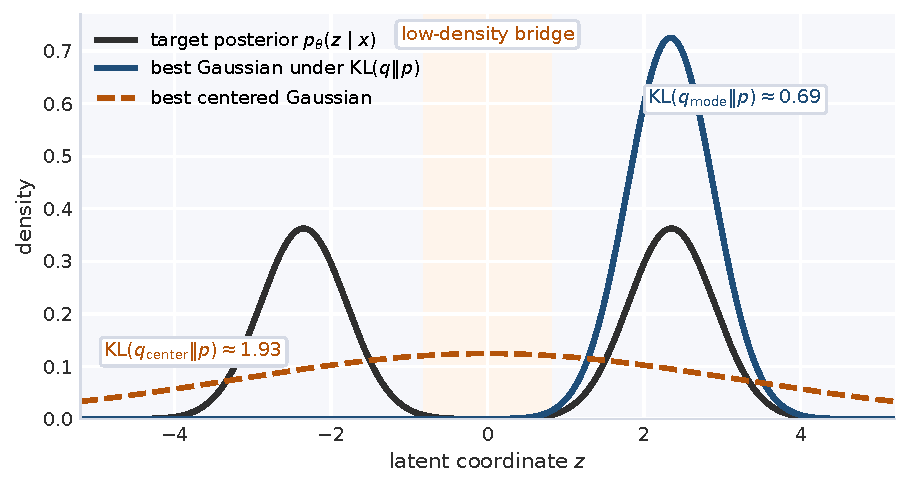
\includegraphics[width=0.92\linewidth]{figures/handouts/elbo_geometry/fig_forward_kl_undercoverage_applied}
  \caption{A bimodal target posterior is approximated by a single Gaussian family.
  The centered Gaussian must place mass in the low-density region between the modes, while the forward-KL minimizer instead concentrates near one mode.
  This is the mode-seeking geometry behind undercoverage.}
  \label{fig:forward-kl-undercoverage-applied}
\end{figure}

In \Cref{fig:forward-kl-undercoverage-applied}, the centered approximation pays for mass throughout the low-density region between the modes, while the forward-KL minimizer avoids that bill and settles on one plausible region.

\begin{exercise}[A three-cell proxy for forward-KL undercoverage]
\label{ex:forward-kl-undercovers}
Approximate a bimodal posterior by three disjoint regions:
\(L\) for the left mode, \(M\) for the low-density middle region, and \(R\) for the right mode.
Suppose
\[
  p(L)=0.49,
  \qquad
  p(M)=0.02,
  \qquad
  p(R)=0.49.
\]
Consider two candidate unimodal approximations:
\[
  q_{\mathrm{mid}}=(0.25,0.50,0.25),
  \qquad
  q_{\mathrm{left}}=(1,0,0),
\]
listed in the order \((L,M,R)\).
\begin{enumerate}[leftmargin=*]
  \item Compute
  \[
    \operatorname{KL}(q_{\mathrm{mid}}\|p)
    =
    \sum_{A\in\{L,M,R\}}
    q_{\mathrm{mid}}(A)\log\frac{q_{\mathrm{mid}}(A)}{p(A)}.
  \]
  \item Compute
  \[
    \operatorname{KL}(q_{\mathrm{left}}\|p).
  \]
  \item Which candidate is preferred by forward KL?
  Explain in one or two sentences which term in the objective makes the centered approximation expensive.
\end{enumerate}
\end{exercise}
\SolutionBox[12]{For the centered candidate,
\[
  \operatorname{KL}(q_{\mathrm{mid}}\|p)
  =
  0.25\log\frac{0.25}{0.49}
  +
  0.50\log\frac{0.50}{0.02}
  +
  0.25\log\frac{0.25}{0.49}
  =
  \frac12\log\frac{625}{49}.
\]
For the left-mode candidate,
\[
  \operatorname{KL}(q_{\mathrm{left}}\|p)
  =
  1\cdot \log\frac{1}{0.49}
  =
  \log\frac{100}{49}.
\]
Numerically,
\[
  \frac12\log\frac{625}{49}\approx 1.27,
  \qquad
  \log\frac{100}{49}\approx 0.71,
\]
so forward KL prefers \(q_{\mathrm{left}}\).
The key penalty is the middle-region term
\[
  0.50\log\frac{0.50}{0.02},
\]
which is large because the centered approximation places substantial mass where the target density is tiny.
This is the discrete version of undercoverage: missing one mode can be cheaper than paying for mass in a low-density middle region.}

The cleanest next example is mean-field VI, where the family deletes dependence before optimization ever starts.

\section{Mean-field deletes dependence before optimization starts}
\label{sec:mean-field-geometry}

\subsection{Factorization is the real approximation}
\label{subsec:mean-field-cavi}

Mean-field VI is the first place where the phrase ``the family is part of the model'' becomes concrete.
Write the latent variable as \(z=(z_1,\dots,z_m)\) and consider the factorized family
\[
  q(z)=\prod_{j=1}^m q_j(z_j).
\]
The point of this choice is not that coordinate ascent is especially deep.
The point is that the posterior is now allowed to move only inside a product geometry.
Any dependence in the true posterior has already been deleted before the optimizer gets to work.

\begin{proposition}[Mean-field coordinate update]
\label{prop:mean-field-update-handout}
Fix all factors except \(q_j\), and assume
\[
  m_j(z_j)\coloneqq \E_{q_{-j}}[\log p_\theta(x,z)]
\]
is finite almost everywhere with \(\int e^{m_j(z_j)}\,dz_j<\infty\).
Then any maximizer of the ELBO over the remaining factor satisfies
\[
  q_j^\star(z_j)
  \propto
  \exp\!\left(
    \E_{q_{-j}}\bigl[\log p_\theta(x,z)\bigr]
  \right),
\]
where the expectation is taken under the current variational law on the remaining coordinates.
\end{proposition}
\begin{proof}
Holding \(q_{-j}\) fixed and optimizing only over \(q_j\), the ELBO becomes
\[
  \mathcal{L}(q;x)
  =
  \int q_j(z_j)\,m_j(z_j)\,dz_j
  -
  \int q_j(z_j)\log q_j(z_j)\,dz_j
  + C,
\]
where \(C\) does not depend on \(q_j\).
Define
\[
  Z_j\coloneqq \int e^{m_j(u)}\,du,
  \qquad
  \widetilde q_j(z_j)\coloneqq Z_j^{-1}e^{m_j(z_j)}.
\]
Then
\[
  \mathcal{L}(q;x)
  =
  -\operatorname{KL}\!\bigl(q_j\,\|\,\widetilde q_j\bigr)+\log Z_j+C,
\]
so the ELBO is maximized at \(q_j=\widetilde q_j\).%
\end{proof}

This is the deterministic analogue of a Gibbs update:
instead of sampling one coordinate from an exact conditional, we replace one factor by the best ELBO fit given the others.
But the more important point is geometric.
Once the family has been factorized, CAVI can only repair the posterior inside that factorized geometry.

\begin{figure}[t]
  \centering
  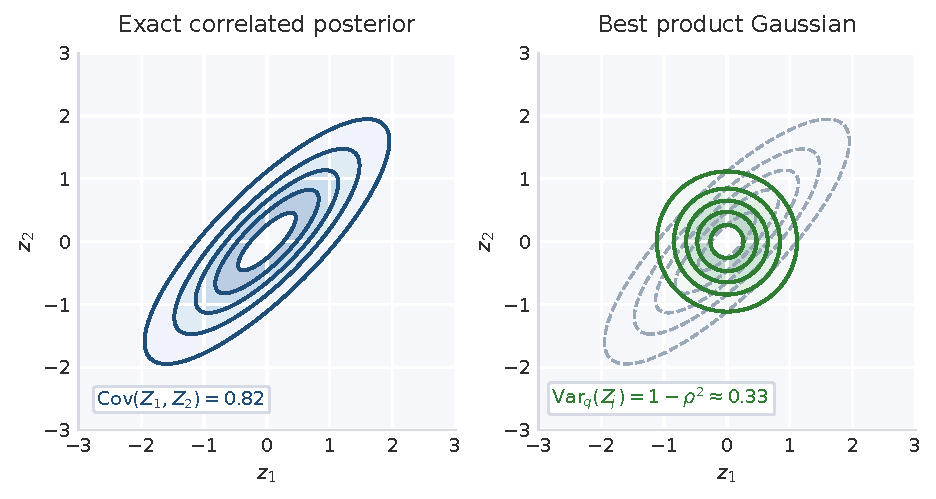
\includegraphics[width=0.92\linewidth]{figures/handouts/elbo_geometry/fig_mean_field_correlation_loss_applied}
  \caption{A correlated Gaussian posterior is compared with the best product Gaussian from the mean-field family.
  The surrogate removes the tilted covariance structure and shrinks each marginal variance, matching the analytic minimizer computed below.}
  \label{fig:mean-field-correlation-loss}
\end{figure}

That loss of geometry is not a training accident.
It is the structural cost of replacing a joint posterior by a product family.
\Cref{fig:mean-field-correlation-loss} shows the cleanest case:
the target posterior is as friendly as possible, but the family is not allowed to tilt.

\begin{proposition}[Best product-Gaussian fit to a correlated Gaussian]
\label{prop:mfvi-gaussian-underdispersion}
Let the exact posterior be
\[
  p_\theta(z\mid x)=\mathcal{N}(0,\Sigma_\rho),
  \qquad
  \Sigma_\rho=
  \begin{bmatrix}
    1 & \rho\\
    \rho & 1
  \end{bmatrix},
  \qquad
  0<|\rho|<1.
\]
Among all fully factorized Gaussian approximations
\[
  q(z_1,z_2)=\mathcal{N}(m_1,s_1^2)\,\mathcal{N}(m_2,s_2^2),
\]
the unique minimizer of
\(\operatorname{KL}(q(z_1,z_2)\|p_\theta(z\mid x))\) satisfies
\[
  m_1=m_2=0,
  \qquad
  s_1^2=s_2^2=1-\rho^2.
\]
In particular, the optimal mean-field approximation is not only uncorrelated; it is also under-dispersed in each coordinate whenever \(\rho\neq 0\).
\end{proposition}
\begin{proof}
The precision matrix is
\[
  \Sigma_\rho^{-1}
  =
  \frac{1}{1-\rho^2}
  \begin{bmatrix}
    1 & -\rho\\
    -\rho & 1
  \end{bmatrix}.
\]
A direct Gaussian-KL calculation gives
\[
  \operatorname{KL}(q\|p_\theta(\cdot\mid x))
  =
  \frac12\left[
    \frac{m_1^2-2\rho m_1m_2+m_2^2+s_1^2+s_2^2}{1-\rho^2}
    -2
    +
    \log\!\frac{1-\rho^2}{s_1^2s_2^2}
  \right].
\]
The quadratic form in \((m_1,m_2)\) is minimized uniquely at \(m_1=m_2=0\).
For \(j\in\{1,2\}\),
\[
  \frac{\partial}{\partial s_j^2}\operatorname{KL}(q\|p_\theta(\cdot\mid x))
  =
  \frac12\left(\frac{1}{1-\rho^2}-\frac{1}{s_j^2}\right),
\]
so the unique stationary point is \(s_j^2=1-\rho^2\).
Since the second derivative with respect to \(s_j^2\) is \(1/(2s_j^4)>0\), this stationary point is the global minimizer.%
\end{proof}

This calculation says exactly what the picture suggests.
The best product approximation cannot reproduce the tilted covariance geometry, so it compensates by shrinking the marginal variances.
Even in the Gaussian case, forward KL plus factorization produces an axis-aligned, overconfident surrogate.

\begin{exercise}[Recover the best product Gaussian]
\label{ex:mean-field-removes-dependence}
Use the displayed formula
\[
  \operatorname{KL}(q\|p_\theta(\cdot\mid x))
  =
  \frac12\left[
    \frac{m_1^2-2\rho m_1m_2+m_2^2+s_1^2+s_2^2}{1-\rho^2}
    -2
    +
    \log\!\frac{1-\rho^2}{s_1^2s_2^2}
  \right]
\]
for the factorized Gaussian \(q(z)=\mathcal{N}(m_1,s_1^2)\mathcal{N}(m_2,s_2^2)\).
\begin{enumerate}[leftmargin=*]
  \item Holding \(s_1^2,s_2^2\) fixed, differentiate with respect to \(m_1,m_2\) and show that the unique stationary point is \(m_1=m_2=0\).
  \item Differentiate with respect to \(s_1^2\) and \(s_2^2\) and show that the minimizer satisfies
  \[
    s_1^2=s_2^2=1-\rho^2.
  \]
  \item Compare these values with the exact posterior variances and covariance. What two geometric distortions does the best product approximation impose?
\end{enumerate}
\end{exercise}
\SolutionBox[12]{Differentiating the KL with respect to the means gives
\[
  \frac{\partial}{\partial m_1}\operatorname{KL}(q\|p_\theta(\cdot\mid x))
  =
  \frac{m_1-\rho m_2}{1-\rho^2},
  \qquad
  \frac{\partial}{\partial m_2}\operatorname{KL}(q\|p_\theta(\cdot\mid x))
  =
  \frac{m_2-\rho m_1}{1-\rho^2}.
\]
The stationary conditions are
\[
  m_1=\rho m_2,
  \qquad
  m_2=\rho m_1.
\]
Since \(|\rho|<1\), the unique solution is \(m_1=m_2=0\).
For the variances,
\[
  \frac{\partial}{\partial s_j^2}\operatorname{KL}(q\|p_\theta(\cdot\mid x))
  =
  \frac12\left(\frac{1}{1-\rho^2}-\frac{1}{s_j^2}\right),
  \qquad j\in\{1,2\},
\]
so the stationary point is \(s_1^2=s_2^2=1-\rho^2\), which is the minimizer.
The exact posterior has marginal variances \(1\) and covariance \(\rho\), while the best product approximation has variances \(1-\rho^2<1\) and covariance \(0\).
So mean-field imposes two distortions at once: it deletes posterior dependence and it shrinks each marginal variance below the true one.}

Up to this point every failure has been local:
one observation, one posterior, one restricted family.
Amortization adds a second restriction across data.

\section{Shared encoders and one latent bottleneck}
\label{sec:shared-encoder-bottleneck}

\subsection{Amortization adds a second restriction}
\label{subsec:amortization-gap}

Amortized VI replaces per-datum variational optimization by a shared encoder \(q_\phi(z\mid x)\).
That makes inference scalable, but it also means that all posterior approximations must lie on the image of one learned map \(x\mapsto q_\phi(\cdot\mid x)\).
On a data set \(x_1,\dots,x_n\), the optimization problem becomes
\[
  \max_{\phi\in\Phi}\sum_{i=1}^n \mathcal{L}(q_\phi(\cdot\mid x_i);x_i)
  \qquad\text{instead of}\qquad
  \sum_{i=1}^n \max_{q\in\mathcal{Q}} \mathcal{L}(q;x_i).
\]
So amortization is not just a faster optimizer for the same approximation problem.
It is a smaller approximation problem.

\begin{figure}[t]
  \centering
  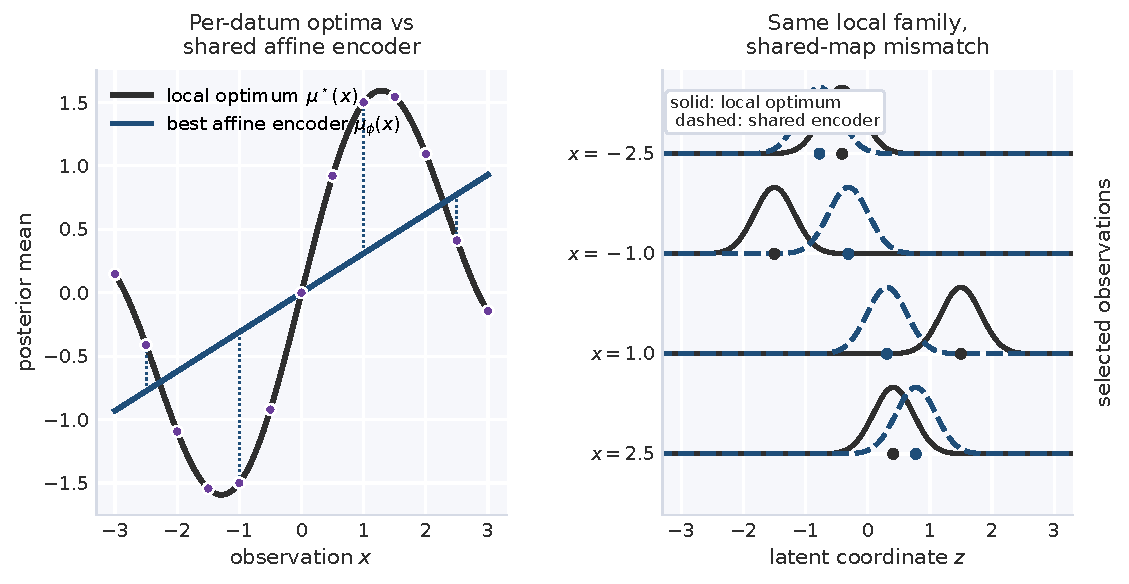
\includegraphics[width=\linewidth]{figures/handouts/elbo_geometry/fig_vi_amortization_applied}
  \caption{A synthetic posterior family with nonlinear per-datum optima \(\mu^\star(x)\) is approximated by a shared affine encoder family.
  The local posteriors are individually representable, but one shared map cannot hit all of the targets simultaneously.
  This is the amortization gap.}
  \label{fig:vi-amortization-handout}
\end{figure}

\Cref{fig:vi-amortization-handout} separates two failure modes that are easy to conflate.
The local family may be adequate for each datum, yet the shared encoder may still miss the local optimum because one map cannot bend in all the required directions at once.

\begin{proposition}[Amortization cannot beat per-datum variational optima]
\label{prop:amortization-gap}
Let \(x_1,\dots,x_n\) be observations, and let \(\mathcal{Q}\) be a variational family available for each datum individually.
Define
\[
  \mathcal{L}_i^\star \coloneqq \sup_{q\in\mathcal{Q}} \mathcal{L}(q;x_i).
\]
Then for any amortized family \(\{q_\phi(\cdot\mid x):\phi\in\Phi\}\subseteq \mathcal{Q}\),
\[
  \sup_{\phi\in\Phi} \sum_{i=1}^n \mathcal{L}(q_\phi(\cdot\mid x_i);x_i)
  \le
  \sum_{i=1}^n \mathcal{L}_i^\star.
\]
\end{proposition}
\begin{proof}
Fix \(\phi\).
For each \(i\), the distribution \(q_\phi(\cdot\mid x_i)\) belongs to \(\mathcal{Q}\), so
\[
  \mathcal{L}(q_\phi(\cdot\mid x_i);x_i)\le \mathcal{L}_i^\star.
\]
Summing over \(i\) gives
\[
  \sum_{i=1}^n \mathcal{L}(q_\phi(\cdot\mid x_i);x_i)\le \sum_{i=1}^n \mathcal{L}_i^\star.
\]
Taking the supremum over \(\phi\) preserves the inequality.%
\end{proof}

The proposition is simple, but it is the correct formal separation between family mismatch and amortization gap.
The gap vanishes only if one shared encoder hits the per-datum optimum everywhere.
Computationally, amortization is still the right idea:
the recognition model and the reparameterized gradient estimator from AEVB and stochastic backpropagation make \(\mathcal{J}(\theta,\phi)\) trainable at scale
\citep[\S\S2.1--2.3]{kingma_welling_2014_aevb}
\citep[\S\S1, 3]{rezende_mohamed_wierstra_2014_stochastic_backpropagation}.
But neither device removes the underlying geometric restriction.

\begin{exercise}[Decompose local mismatch and amortization gap]
\label{ex:amortization-gap}
Let
\[
  \mathcal{L}_i^\star
  \coloneqq
  \sup_{q\in\mathcal{Q}}\mathcal{L}(q;x_i),
  \qquad i=1,\dots,n.
\]
Define the local approximation gap
\[
  \Delta_i^{\mathrm{loc}}
  \coloneqq
  \log p_\theta(x_i)-\mathcal{L}_i^\star
\]
and the amortization gap
\[
  \Delta_{\mathrm{am}}
  \coloneqq
  \sum_{i=1}^n \mathcal{L}_i^\star
  -
  \sup_{\phi\in\Phi}\sum_{i=1}^n \mathcal{L}(q_\phi(\cdot\mid x_i);x_i).
\]
Assume the amortized family satisfies
\[
  \{q_\phi(\cdot\mid x_i):\phi\in\Phi\}\subseteq \mathcal{Q}
  \qquad\text{for every }i.
\]
\begin{enumerate}[leftmargin=*]
  \item Use the ELBO--KL identity to show that, for each \(i\),
  \[
    \Delta_i^{\mathrm{loc}}
    =
    \inf_{q\in\mathcal{Q}}
    \operatorname{KL}\!\bigl(q(z)\,\|\,p_\theta(z\mid x_i)\bigr),
  \]
  and in particular \(\Delta_i^{\mathrm{loc}}\ge 0\).
  \item Use \Cref{prop:amortization-gap} to show \(\Delta_{\mathrm{am}}\ge 0\).
  \item Fix \(\phi\). Show that for each \(i\),
  \[
    \mathcal{L}(q_\phi(\cdot\mid x_i);x_i)\le \mathcal{L}_i^\star.
  \]
  Then sum over \(i\) and take the supremum over \(\phi\) to recover the inequality
  \[
    \sup_{\phi\in\Phi}\sum_{i=1}^n \mathcal{L}(q_\phi(\cdot\mid x_i);x_i)
    \le
    \sum_{i=1}^n \mathcal{L}_i^\star.
  \]
  \item Prove the exact decomposition
  \[
    \sum_{i=1}^n \log p_\theta(x_i)
    -
    \sup_{\phi\in\Phi}\sum_{i=1}^n \mathcal{L}(q_\phi(\cdot\mid x_i);x_i)
    =
    \sum_{i=1}^n \Delta_i^{\mathrm{loc}}
    +
    \Delta_{\mathrm{am}}.
  \]
  \item Explain what vanishes in the two extreme cases:
  a purely local-family-limited regime and a purely amortization-limited regime.
\end{enumerate}
\end{exercise}
\SolutionBox[15]{By the ELBO--KL identity,
\[
  \log p_\theta(x_i)
  =
  \mathcal{L}(q;x_i)
  +
  \operatorname{KL}\!\bigl(q(z)\,\|\,p_\theta(z\mid x_i)\bigr)
\]
for every admissible \(q\in\mathcal{Q}\).
Taking the supremum over \(q\in\mathcal{Q}\) on the ELBO side is the same as taking the infimum of the KL term, so
\[
  \Delta_i^{\mathrm{loc}}
  =
  \log p_\theta(x_i)-\mathcal{L}_i^\star
  =
  \inf_{q\in\mathcal{Q}}
  \operatorname{KL}\!\bigl(q(z)\,\|\,p_\theta(z\mid x_i)\bigr)\ge 0.
\]
Next,
\[
  \Delta_{\mathrm{am}}
  =
  \sum_{i=1}^n \mathcal{L}_i^\star
  -
  \sup_{\phi\in\Phi}\sum_{i=1}^n \mathcal{L}(q_\phi(\cdot\mid x_i);x_i)\ge 0
\]
by \Cref{prop:amortization-gap}.
Fix \(\phi\).
For each datum \(x_i\), the distribution \(q_\phi(\cdot\mid x_i)\) belongs to \(\mathcal{Q}\), so by definition of \(\mathcal{L}_i^\star\),
\[
  \mathcal{L}(q_\phi(\cdot\mid x_i);x_i)\le \mathcal{L}_i^\star.
\]
Summing over \(i\) gives
\[
  \sum_{i=1}^n \mathcal{L}(q_\phi(\cdot\mid x_i);x_i)
  \le
  \sum_{i=1}^n \mathcal{L}_i^\star.
\]
Taking the supremum over \(\phi\) preserves the inequality and yields the claim.
For the exact decomposition, add and subtract \(\sum_i \mathcal{L}_i^\star\):
\begin{align*}
  \sum_{i=1}^n \log p_\theta(x_i)
  -
  \sup_{\phi}\sum_{i=1}^n \mathcal{L}(q_\phi(\cdot\mid x_i);x_i)
  &=
  \sum_{i=1}^n \bigl(\log p_\theta(x_i)-\mathcal{L}_i^\star\bigr) \\
  &\quad
  +
  \sum_{i=1}^n \mathcal{L}_i^\star
  -
  \sup_{\phi}\sum_{i=1}^n \mathcal{L}(q_\phi(\cdot\mid x_i);x_i) \\
  &=
  \sum_{i=1}^n \Delta_i^{\mathrm{loc}}+\Delta_{\mathrm{am}}.
\end{align*}
In a purely local-family-limited regime, \(\Delta_{\mathrm{am}}=0\) and the whole gap comes from the local family \(\mathcal{Q}\) being too small.
In a purely amortization-limited regime, every \(\Delta_i^{\mathrm{loc}}=0\) and the whole gap comes from one shared encoder failing to realize the per-datum optima.}

\subsection{Blur: overlapping latent neighborhoods force averaging}
\label{subsec:blur}

From this point on, keep the standard one-bottleneck VAE in mind:
a prior \(p(z)\), decoder \(p_\theta(x\mid z)\), and shared encoder \(q_\phi(z\mid x)\).
This is the AEVB setting with the usual reparameterization
\[
  z=\mu_\phi(x)+\sigma_\phi(x)\odot \varepsilon,
  \qquad
  \varepsilon\sim\mathcal{N}(0,I),
\]
which makes stochastic ELBO optimization practical but does not alter the geometry of the approximation problem
\citep[\S\S2.1--2.3]{kingma_welling_2014_aevb}
\citep[\S3]{rezende_mohamed_wierstra_2014_stochastic_backpropagation}.

The blur mechanism becomes sharp when the decoder is Gaussian.
Then, for fixed \(q_\phi\), decoder learning is literally a regression problem under the joint law induced by the data and the encoder.
That is the direct link from ``posterior overlap'' to blurry reconstructions.

\begin{proposition}[A fixed-encoder Gaussian VAE is regression under \(p_{\mathrm{data}}(x)q_\phi(z\mid x)\)]
\label{prop:gaussian-vae-regression}
Assume \(\sigma^2>0\) is fixed and
\[
  p_\theta(x\mid z)=\mathcal{N}\!\bigl(\mu_\theta(z),\sigma^2 I\bigr).
\]
Then the expected ELBO over the data distribution satisfies
\[
  \E_{p_{\mathrm{data}}(x)}\!\bigl[\mathcal{L}(q_\phi;x)\bigr]
  =
  C(\phi,\sigma^2)
  -
  \frac{1}{2\sigma^2}
  \E_{(X,Z)\sim \pi_\phi}\!\bigl[\norm{X-\mu_\theta(Z)}_2^2\bigr],
\]
where
\[
  \pi_\phi(dx,dz)\coloneqq p_{\mathrm{data}}(x)\,q_\phi(dz\mid x)
\]
and
\[
  C(\phi,\sigma^2)
  =
  -\frac{d}{2}\log(2\pi\sigma^2)
  -
  \E_{p_{\mathrm{data}}(x)}
  \operatorname{KL}\!\bigl(q_\phi(z\mid x)\,\|\,p(z)\bigr)
\]
does not depend on \(\mu_\theta\).
Consequently, for fixed \(q_\phi\), maximizing the expected ELBO over decoder means \(\mu_\theta\) is equivalent to minimizing
\[
  \mu\mapsto
  \E_{(X,Z)\sim \pi_\phi}\!\bigl[\norm{X-\mu(Z)}_2^2\bigr].
\]
\end{proposition}
\begin{proof}
For each \(x\),
\[
  \mathcal{L}(q_\phi;x)
  =
  \E_{q_\phi(z\mid x)}[\log p_\theta(x\mid z)]
  -
  \operatorname{KL}\!\bigl(q_\phi(z\mid x)\,\|\,p(z)\bigr).
\]
Under the Gaussian decoder,
\[
  \log p_\theta(x\mid z)
  =
  -\frac{d}{2}\log(2\pi\sigma^2)
  -
  \frac{1}{2\sigma^2}\norm{x-\mu_\theta(z)}_2^2.
\]
Taking expectations over \(p_{\mathrm{data}}(x)\) gives
\begin{align*}
  \E_{p_{\mathrm{data}}(x)}\!\bigl[\mathcal{L}(q_\phi;x)\bigr]
  &=
  -\frac{d}{2}\log(2\pi\sigma^2)
  -
  \frac{1}{2\sigma^2}
  \E_{p_{\mathrm{data}}(x)q_\phi(z\mid x)}
  \norm{x-\mu_\theta(z)}_2^2 \\
  &\quad
  -
  \E_{p_{\mathrm{data}}(x)}
  \operatorname{KL}\!\bigl(q_\phi(z\mid x)\,\|\,p(z)\bigr),
\end{align*}
which is the stated identity.%
\end{proof}

\begin{proposition}[Squared loss chooses conditional means]
\label{prop:squared-error-mean}
Let \((X,Z)\) be jointly distributed with \(X\in\R^d\), \(Z\in\R^m\), and \(\E\norm{X}_2^2<\infty\).
Among all measurable maps \(\mu:\R^m\to\R^d\) such that \(\E\norm{\mu(Z)}_2^2<\infty\), the minimizer of
\[
  \mu\mapsto \E\norm{X-\mu(Z)}_2^2
\]
satisfies
\[
  \mu^\star(Z)=\E[X\mid Z]
\]
almost surely, where \(\E[X\mid Z]\) denotes any version of the conditional expectation.
\end{proposition}
\begin{proof}
For any measurable \(\mu\),
\begin{align*}
  \E\norm{X-\mu(Z)}_2^2
  &=
  \E\norm{X-\E[X\mid Z]}_2^2
  +
  \E\norm{\E[X\mid Z]-\mu(Z)}_2^2 \\
  &\quad
  +
  2\,\E\!\left[
    \ip{X-\E[X\mid Z]}{\E[X\mid Z]-\mu(Z)}
  \right].
\end{align*}
The cross term vanishes because
\[
  \E\!\left[X-\E[X\mid Z]\mid Z\right]=0
\]
and \(\E[X\mid Z]-\mu(Z)\) is \(Z\)-measurable.
Therefore
\[
  \E\norm{X-\mu(Z)}_2^2
  =
  \E\norm{X-\E[X\mid Z]}_2^2
  +
  \E\norm{\E[X\mid Z]-\mu(Z)}_2^2,
\]
so the minimum is attained exactly when \(\mu(Z)=\E[X\mid Z]\) almost surely.%
\end{proof}

\Cref{prop:gaussian-vae-regression} and \Cref{prop:squared-error-mean} give the blur mechanism in one line:
for fixed \(q_\phi\), a Gaussian decoder mean that minimizes the reconstruction risk is any version of
\[
  \mu_\theta^\star(Z)=\E_{\pi_\phi}[X\mid Z]
\]
almost surely.
So if the encoder geometry pushes several incompatible observations into the same latent neighborhood, the decoder is forced toward a conditional mean rather than any one sharp sample.
This makes precise the ``posterior overlap'' and ``locality'' story emphasized in the \(\beta\)-VAE discussion of \citet[\S\S4.2--5]{burgess_higgins_pal_matthey_watters_desjardins_lerchner_2018_understanding_bvae}.

\subsubsection{A two-point blur example}
\label{subsubsec:two-point-blur}

The abstract conditional-mean statement becomes concrete in the smallest nontrivial example.
If one latent neighborhood mixes two genuinely different observations, the decoder has no sharper target available than their average.

\begin{example}[Ambiguity forces averaging]
\label{ex:two-point-blur}
Suppose the data distribution places probability \(1/2\) on \(x^{(1)}\in\R^d\) and probability \(1/2\) on \(x^{(2)}\in\R^d\), and suppose that a version of the conditional law of \(X\) given \(Z\) satisfies, at some latent location \(z\),
\[
  \Pr(X=x^{(1)}\mid Z=z)
  =
  \Pr(X=x^{(2)}\mid Z=z)
  =
  \frac12.
\]
Then a risk-minimizing Gaussian-decoder prediction at that latent point is
\[
  \mu_\theta(z)
  =
  \E[X\mid Z=z]
  =
  \frac{x^{(1)}+x^{(2)}}{2}.
\]
Unless \(x^{(1)}=x^{(2)}\), the reconstruction is an average rather than an actual datum.
\end{example}

The example is tiny, but it captures the full story.
Blur does not mean the decoder is inherently bad at detail.
It means the encoder geometry failed to separate distinctions that matter to squared-error reconstruction.
When the bottleneck has too little effective capacity, the decoder is rewarded for averaging unresolved variation
\citep[\S\S4.2--5]{burgess_higgins_pal_matthey_watters_desjardins_lerchner_2018_understanding_bvae}.

\begin{figure}[t]
  \centering
  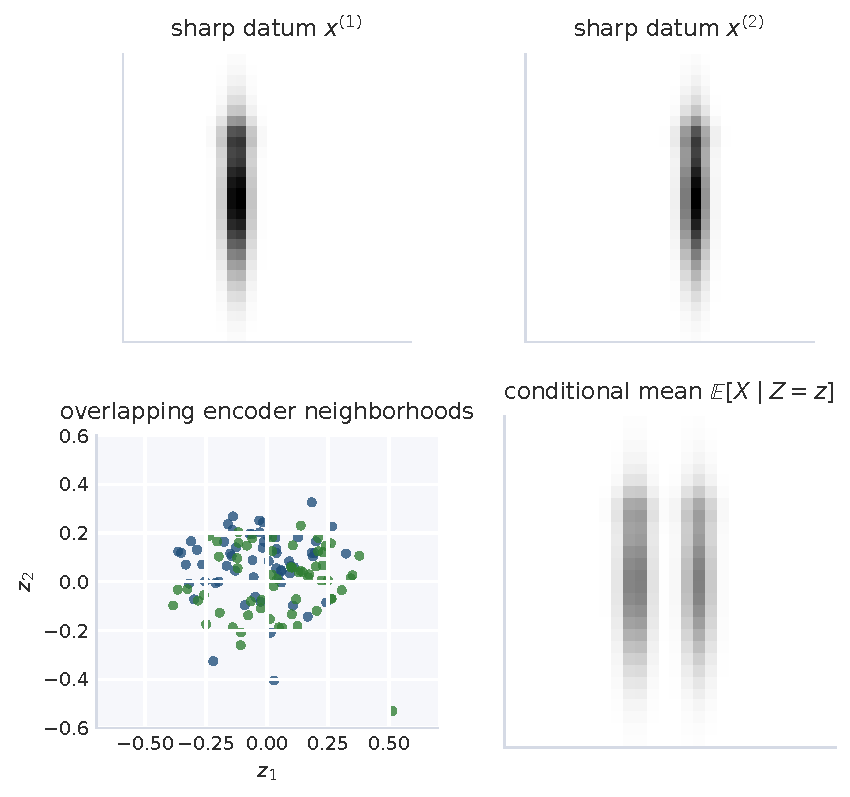
\includegraphics[width=0.84\linewidth]{figures/handouts/elbo_geometry/fig_latent_overlap_blur_applied}
  \caption{Two distinct sharp observations are mapped into nearly the same latent neighborhood.
  A Gaussian decoder therefore returns their conditional mean, which is visibly blurrier than either endpoint.}
  \label{fig:latent-overlap-blur}
\end{figure}

\begin{exercise}[The irreducible blur penalty]
\label{ex:blur-average}
In the two-point example above, show the exact identity
\[
  \frac12\norm{x^{(1)}-a}_2^2+\frac12\norm{x^{(2)}-a}_2^2
  =
  \frac14\norm{x^{(1)}-x^{(2)}}_2^2
  +
  \norm{a-\tfrac12(x^{(1)}+x^{(2)})}_2^2.
\]
Deduce that the minimizer is \(a=(x^{(1)}+x^{(2)})/2\) and compute the minimum value explicitly in terms of \(\norm{x^{(1)}-x^{(2)}}_2\).
Then explain how this finite identity mirrors the decomposition in \Cref{prop:squared-error-mean}.
\end{exercise}
\SolutionBox[9]{Expanding the quadratic gives
\[
  \frac12\norm{x^{(1)}-a}_2^2+\frac12\norm{x^{(2)}-a}_2^2
  =
  \frac14\norm{x^{(1)}-x^{(2)}}_2^2
  +
  \norm{a-\tfrac12(x^{(1)}+x^{(2)})}_2^2.
\]
Hence the minimizer is the midpoint \(a=(x^{(1)}+x^{(2)})/2\).
The minimum value is
\[
  \frac14\norm{x^{(1)}-x^{(2)}}_2^2.
\]
This is the two-point version of \Cref{prop:squared-error-mean}: the first term is the irreducible conditional-variance cost, and the second term is the extra penalty for choosing a prediction different from the conditional mean.
So even the best decoder incurs a positive reconstruction penalty whenever distinct observations share one latent code.}

\subsection{Collapse: the decoder can make latent information too expensive}
\label{subsec:collapse}

Blur and collapse are opposite-looking symptoms of the same bottleneck picture.
In blur, the latent code is used but is not expressive enough to separate incompatible observations.
In collapse, the decoder becomes so strong that using \(z\) is not worth the KL bill.
The cleanest formal toy case is when the decoder literally ignores \(z\).

\begin{proposition}[If the decoder ignores \(z\), the ELBO prefers the prior]
\label{prop:collapse-if-decoder-ignores-z}
Suppose \(p_\theta(x\mid z)=p_\theta(x)\) for all \(z\).
Then for every \(x\),
\[
  \mathcal{L}(q;x)=\log p_\theta(x)-\operatorname{KL}\!\bigl(q(z)\,\|\,p(z)\bigr),
\]
so the ELBO is maximized by \(q(z)=p(z)\).
\end{proposition}
\begin{proof}
Under the assumption \(p_\theta(x\mid z)=p_\theta(x)\),
\[
  p_\theta(x,z)=p_\theta(x)\,p(z).
\]
Substituting this into the ELBO gives
\[
  \mathcal{L}(q;x)
  =
  \E_q[\log p_\theta(x)+\log p(z)-\log q(z)]
  =
  \log p_\theta(x)-\operatorname{KL}\!\bigl(q(z)\,\|\,p(z)\bigr).
\]
The KL term is minimized at \(q(z)=p(z)\), proving the claim.%
\end{proof}

Real posterior collapse is usually less extreme than this toy case, but the geometry is the same.
If the decoder can already explain \(x\) well enough on its own, then the ELBO charges for transmitting information through \(z\) without demanding much in return.
The latent variable becomes expendable.

To see the bill more clearly, average the KL term over the data distribution and define the aggregate posterior
\[
  q_\phi(z)
  \coloneqq
  \int q_\phi(z\mid x)\,p_{\mathrm{data}}(x)\,dx.
\]

\begin{proposition}[Mutual-information decomposition of the KL term]
\label{prop:mi-decomposition}
Assume \(q_\phi(z\mid x)\) and \(p(z)\) are densities with respect to a common base measure and that the displayed expectations are finite.
We have
\[
  \E_{p_{\mathrm{data}}(x)}
  \operatorname{KL}\!\bigl(q_\phi(z\mid x)\,\|\,p(z)\bigr)
  =
  I_q(X;Z)
  +
  \operatorname{KL}\!\bigl(q_\phi(z)\,\|\,p(z)\bigr),
\]
where \(I_q(X;Z)\) is mutual information under the joint law
\[
  p_{\mathrm{data}}(x)\,q_\phi(z\mid x).
\]
\end{proposition}
\begin{proof}
Expand the left-hand side:
\[
  \E_{p_{\mathrm{data}}(x)q_\phi(z\mid x)}
  \bigl[\log q_\phi(z\mid x)-\log p(z)\bigr].
\]
Add and subtract \(\log q_\phi(z)\):
\[
  \E\!\bigl[\log q_\phi(z\mid x)-\log q_\phi(z)\bigr]
  +
  \E\!\bigl[\log q_\phi(z)-\log p(z)\bigr].
\]
The first term is \(I_q(X;Z)\), and the second is
\(\operatorname{KL}(q_\phi(z)\|p(z))\).%
\end{proof}

Combining \Cref{prop:mi-decomposition} with the expected ELBO gives
\[
  \E_{p_{\mathrm{data}}(x)}\!\bigl[\mathcal{L}(q_\phi;x)\bigr]
  =
  \E_{p_{\mathrm{data}}(x)q_\phi(z\mid x)}[\log p_\theta(x\mid z)]
  -
  I_q(X;Z)
  -
  \operatorname{KL}\!\bigl(q_\phi(z)\,\|\,p(z)\bigr).
\]
So the KL regularizer is charging for two things at once:
how much information the code stores about the data, and how far the aggregate code distribution drifts from the prior.
If the decoder class already contains good nearly unconditional models for the data, the collapsed solution can be globally competitive; more generally, using \(z\) is worthwhile only when the reconstruction gain beats this information bill.

This helps explain why expressive autoregressive decoders often collapse in practice.
Bowman et al.\ show the sentence-VAE version of this story:
if the decoder is already a strong language model, training pushes \(q_\phi(z\mid x)\) back toward the prior unless the optimization pressure is modified
\citep[\S3.1]{bowman_vilnis_vinyals_dai_jozefowicz_bengio_2016_generating_sentences}.
He et al.\ give the complementary dynamic explanation:
early in training the decoder can move faster than the inference network, and that lag can steer the system into a collapsed regime before the encoder learns to use \(z\)
\citep[\S\S3--4]{he_spokoyny_neubig_bergkirkpatrick_2019_lagging_inference}.

\begin{figure}[t]
  \centering
  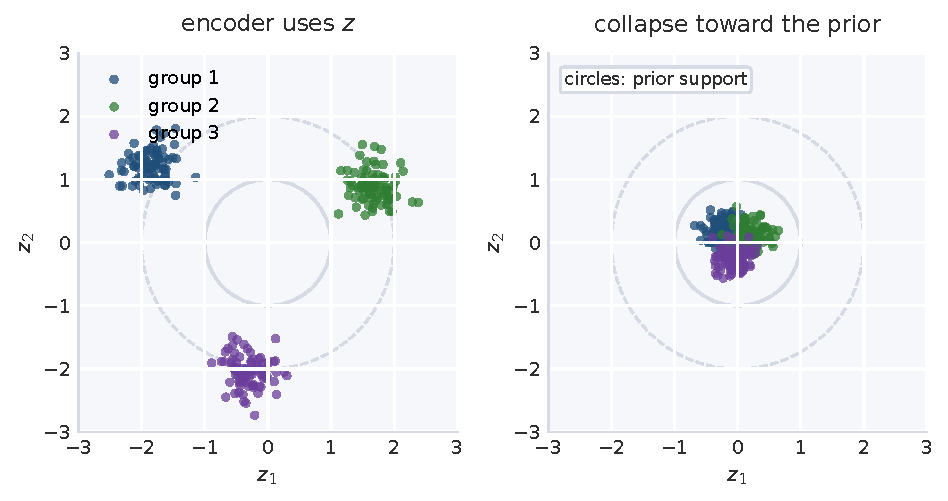
\includegraphics[width=0.90\linewidth]{figures/handouts/elbo_geometry/fig_decoder_bypass_collapse_applied}
  \caption{Toy encoder outputs for three groups of observations.
  When the latent variable is used, the group-conditioned posteriors separate in latent space; under posterior collapse they contract back toward the prior and overlap heavily, so little information about \(x\) remains in \(z\).}
  \label{fig:decoder-bypass-collapse}
\end{figure}

This also clarifies what KL warm-up and \(\beta\)-VAE style heuristics do.
They change the price of information.
That can change which local optimum training reaches, but it does not enlarge the variational family or remove the possibility of collapse
\citep[\S3.1]{bowman_vilnis_vinyals_dai_jozefowicz_bengio_2016_generating_sentences}
\citep[\S\S3--5]{burgess_higgins_pal_matthey_watters_desjardins_lerchner_2018_understanding_bvae}.

\begin{exercise}[\(\beta\)-ELBO as a weighted information budget]
\label{ex:beta-elbo}
Consider the \(\beta\)-ELBO
\[
  \mathcal{L}_\beta(q;x)
  =
  \E_q[\log p_\theta(x\mid z)]
  -
  \beta\,\operatorname{KL}\!\bigl(q(z)\,\|\,p(z)\bigr).
\]
\begin{enumerate}[leftmargin=*]
  \item After averaging over \(p_{\mathrm{data}}(x)\), write the objective as
  \[
    \E_{p_{\mathrm{data}}(x)q_\phi(z\mid x)}[\log p_\theta(x\mid z)]
    -
    \beta\,\E_{p_{\mathrm{data}}(x)}
    \operatorname{KL}\!\bigl(q_\phi(z\mid x)\,\|\,p(z)\bigr).
  \]
  \item In the averaged KL term, add and subtract \(\log q_\phi(z)\) exactly as in the proof of \Cref{prop:mi-decomposition}.
  \item Identify the two resulting terms and conclude that
  \[
    \E_{p_{\mathrm{data}}(x)}[\mathcal{L}_\beta(q_\phi;x)]
    =
    \E_{p_{\mathrm{data}}(x)q_\phi(z\mid x)}[\log p_\theta(x\mid z)]
    -
    \beta\,I_q(X;Z)
    -
    \beta\,\operatorname{KL}\!\bigl(q_\phi(z)\,\|\,p(z)\bigr).
  \]
  \item State separately what large \(\beta\) and small \(\beta\) do to the two non-reconstruction terms.
\end{enumerate}
\end{exercise}
\SolutionBox[10]{Apply \Cref{prop:mi-decomposition} to the averaged KL term:
\[
  \E_{p_{\mathrm{data}}(x)}
  \operatorname{KL}\!\bigl(q_\phi(z\mid x)\,\|\,p(z)\bigr)
  =
  I_q(X;Z)
  +
  \operatorname{KL}\!\bigl(q_\phi(z)\,\|\,p(z)\bigr).
\]
More explicitly,
\[
  \E\!\bigl[\log q_\phi(z\mid x)-\log p(z)\bigr]
  =
  \E\!\bigl[\log q_\phi(z\mid x)-\log q_\phi(z)\bigr]
  +
  \E\!\bigl[\log q_\phi(z)-\log p(z)\bigr],
\]
where the first expectation is \(I_q(X;Z)\) and the second is
\(\operatorname{KL}(q_\phi(z)\|p(z))\).
Substituting into the expected \(\beta\)-ELBO yields
\[
  \E_{p_{\mathrm{data}}(x)}[\mathcal{L}_\beta(q_\phi;x)]
  =
  \E_{p_{\mathrm{data}}(x)q_\phi(z\mid x)}[\log p_\theta(x\mid z)]
  -
  \beta\,I_q(X;Z)
  -
  \beta\,\operatorname{KL}\!\bigl(q_\phi(z)\,\|\,p(z)\bigr).
\]
So \(\beta\) directly rescales both parts of the KL bill.
Large \(\beta\) makes informative codes and prior mismatch expensive, which pushes toward weaker latent usage and can favor collapse.
Small \(\beta\) relaxes both penalties, so the model is more willing to store information in \(z\) and to let the aggregate posterior drift from the prior.
This changes optimization pressure, but it does not enlarge the family \(q_\phi(z\mid x)\), so it does not remove the underlying geometric mismatch.}

\section{Structural redesigns}
\label{sec:structural-redesigns}

Once the problem is framed this way, the right fix is often not ``optimize the same ELBO harder''.
If one latent layer is too coarse, or if learning the encoder geometry itself is unstable, then the approximation problem must change.
Two recurring redesigns do that:
hierarchy and fixed-bridge latent models.

\subsection{Hierarchy splits one overloaded KL bill into local bills}
\label{subsec:hierarchy-redistributes-kl}

A hierarchical VAE replaces one bottleneck by a stack of latent variables.
The key point is not just that the network is deeper.
The important change is that no single latent variable has to pay for every kind of variation at once.
Coarse structure can be represented high in the hierarchy and local detail lower down, so the ELBO decomposes into several local KL penalties instead of one global bottleneck charge.

Consider a hierarchical VAE with latent variables \(z_{1:L}\) and factorization
\[
  p_\theta(x,z_{1:L})
  =
  p_\theta(x\mid z_1)\,
  \prod_{\ell=1}^{L-1} p_\theta(z_\ell\mid z_{\ell+1})\,
  p(z_L),
\]
together with a structured encoder
\[
  q_\phi(z_{1:L}\mid x)
  =
  q_\phi(z_L\mid x)\,
  \prod_{\ell=1}^{L-1} q_\phi(z_\ell\mid z_{\ell+1},x).
\]

\begin{proposition}[Hierarchical ELBO as reconstruction minus local KL terms]
\label{prop:hierarchical-elbo}
For the model and encoder above,
\begin{align*}
  \mathcal{L}(q_\phi;x)
  &=
  \E_{q_\phi}\bigl[\log p_\theta(x\mid z_1)\bigr]
  -
  \operatorname{KL}\!\bigl(q_\phi(z_L\mid x)\,\|\,p(z_L)\bigr) \\
  &\quad
  -
  \sum_{\ell=1}^{L-1}
  \E_{q_\phi(z_{\ell+1:L}\mid x)}\!\left[
    \operatorname{KL}\!\bigl(
      q_\phi(z_\ell\mid z_{\ell+1},x)\,\|\,p_\theta(z_\ell\mid z_{\ell+1})
    \bigr)
  \right].
\end{align*}
\end{proposition}
\begin{proof}
Start from
\[
  \mathcal{L}(q_\phi;x)
  =
  \E_{q_\phi}\!\bigl[\log p_\theta(x,z_{1:L})-\log q_\phi(z_{1:L}\mid x)\bigr].
\]
Substituting the factorizations of \(p_\theta\) and \(q_\phi\) gives
\begin{align*}
  \mathcal{L}(q_\phi;x)
  &=
  \E_{q_\phi}[\log p_\theta(x\mid z_1)] \\
  &\quad
  +
  \E_{q_\phi}\!\left[
    \sum_{\ell=1}^{L-1} \log p_\theta(z_\ell\mid z_{\ell+1})
    + \log p(z_L)
    - \sum_{\ell=1}^{L-1} \log q_\phi(z_\ell\mid z_{\ell+1},x)
    - \log q_\phi(z_L\mid x)
  \right].
\end{align*}
The top-level terms combine as
\[
  \E_{q_\phi}\!\left[\log p(z_L)-\log q_\phi(z_L\mid x)\right]
  =
  -\operatorname{KL}\!\bigl(q_\phi(z_L\mid x)\,\|\,p(z_L)\bigr).
\]
For each \(\ell\in\{1,\dots,L-1\}\),
\begin{align*}
  &\E_{q_\phi}\!\left[
    \log p_\theta(z_\ell\mid z_{\ell+1})
    -
    \log q_\phi(z_\ell\mid z_{\ell+1},x)
  \right] \\
  &\qquad
  =
  -\E_{q_\phi(z_{\ell+1:L}\mid x)}\!\left[
    \operatorname{KL}\!\bigl(
      q_\phi(z_\ell\mid z_{\ell+1},x)\,\|\,p_\theta(z_\ell\mid z_{\ell+1})
    \bigr)
  \right].
\end{align*}
Substituting these identities back into the ELBO gives the result.%
\end{proof}

\Cref{prop:hierarchical-elbo} is the structural point in formula form.
The ELBO no longer contains one global penalty that forces a single latent variable to trade off every kind of information simultaneously.
Instead it contains a top-level prior-matching term and a sum of local conditional KL penalties.
That is why hierarchy can relieve both blur and collapse:
different scales of variation can be distributed across levels rather than compressed through one code.
This is exactly the design philosophy behind deep hierarchical VAEs such as NVAE, where global structure is represented high in the hierarchy and local detail is refined lower down
\citep[\S3.1]{vahdat_kautz_2020_nvae}.

\begin{figure}[t]
  \centering
  \begin{tikzpicture}[>=Stealth,font=\footnotesize]
  \tikzset{
    elbopanel/.style={
      draw=stat221Gray!30,
      fill=white,
      rounded corners=5pt,
      line width=0.6pt
    },
    elbotitle/.style={font=\small\bfseries, text=stat221Gray!90},
    latbox/.style={
      rounded corners=3pt,
      minimum width=1.95cm,
      minimum height=0.76cm,
      line width=0.8pt
    },
    elbobadge/.style={
      rounded corners=2pt,
      inner sep=2.6pt,
      font=\footnotesize,
      align=center,
      text=stat221Gray!85
    }
  }
  \path[use as bounding box] (-0.15,-0.24) rectangle (13.45,5.15);

  \node[elbopanel,minimum width=4.10cm,minimum height=4.95cm,anchor=north west] (leftpanel) at (0.0,4.85) {};
  \node[elbopanel,minimum width=4.10cm,minimum height=4.95cm,anchor=north west] (midpanel) at (4.62,4.85) {};
  \node[elbopanel,minimum width=4.10cm,minimum height=4.95cm,anchor=north west] (rightpanel) at (9.24,4.85) {};

  \node[elbotitle,anchor=north west] at ([xshift=0.25cm,yshift=-0.28cm]leftpanel.north west) {Single bottleneck};
  \node[elbotitle,anchor=north west] at ([xshift=0.25cm,yshift=-0.28cm]midpanel.north west) {Hierarchy splits scales};
  \node[elbotitle,anchor=north west] at ([xshift=0.25cm,yshift=-0.28cm]rightpanel.north west) {Cleaner allocation};

  \node[latbox,draw=stat221Purple!72!black,fill=stat221PurpleLight,minimum width=1.18cm,minimum height=0.68cm] (coarse) at (0.95,3.15) {class};
  \node[latbox,draw=stat221Blue!72!black,fill=stat221BlueLight,minimum width=1.28cm,minimum height=0.68cm] (detail) at (2.05,3.15) {detail};
  \node[latbox,draw=stat221Orange!78!black,fill=stat221OrangeLight,minimum width=1.22cm,minimum height=0.68cm] (noise) at (3.15,3.15) {noise};
  \node[latbox,draw=stat221Purple!72!black,fill=stat221PurpleLight,minimum width=2.15cm,minimum height=0.88cm] (z) at (2.05,1.95) {$z$};
  \node[latbox,draw=stat221Green!68!black,fill=stat221GreenLight,minimum width=2.15cm,minimum height=0.88cm] (x) at (2.05,0.75) {$x$};
  \draw[->,stat221Gray!75,line width=0.85pt] (coarse.south) -- (z.north west);
  \draw[->,stat221Gray!75,line width=0.85pt] (detail.south) -- (z.north);
  \draw[->,stat221Gray!75,line width=0.85pt] (noise.south) -- (z.north east);
  \draw[->,stat221Gray!75,line width=0.85pt] (z) -- (x);
  \node[elbobadge,fill=stat221Gray!8,anchor=west] at (2.72,1.30) {one KL budget};

  \node[latbox,draw=stat221Purple!72!black,fill=stat221PurpleLight,minimum width=2.05cm,minimum height=0.88cm] (z2) at (6.68,3.05) {$z_2$};
  \node[latbox,draw=stat221Blue!72!black,fill=stat221BlueLight,minimum width=2.05cm,minimum height=0.88cm] (z1) at (6.68,1.92) {$z_1$};
  \node[latbox,draw=stat221Green!68!black,fill=stat221GreenLight,minimum width=2.05cm,minimum height=0.88cm] (xh) at (6.68,0.78) {$x$};
  \draw[->,stat221Gray!75,line width=0.85pt] (z2) -- (z1);
  \draw[->,stat221Gray!75,line width=0.85pt] (z1) -- (xh);
  \node[elbobadge,fill=stat221PurpleLight,anchor=east,text=stat221Purple!75!black] at (5.28,3.05) {global};
  \node[elbobadge,fill=stat221BlueLight,anchor=east,text=stat221Blue!75!black] at (5.28,1.92) {local};
  \node[elbobadge,fill=stat221Gray!8,anchor=west] at (7.42,2.47) {$\operatorname{KL}_2$};
  \node[elbobadge,fill=stat221Gray!8,anchor=west] at (7.42,1.34) {$\operatorname{KL}_1$};

  \node[latbox,draw=stat221Purple!72!black,fill=stat221PurpleLight,text width=1.05cm,align=center,inner xsep=2.6pt] (cat1) at (10.31,3.00) {class 1};
  \node[latbox,draw=stat221Purple!72!black,fill=stat221PurpleLight,text width=1.05cm,align=center,inner xsep=2.6pt] (cat2) at (12.26,3.00) {class 2};
  \node[latbox,draw=stat221Blue!72!black,fill=stat221BlueLight,minimum width=0.98cm,minimum height=0.60cm,inner xsep=1.2pt] (d11) at (9.86,1.45) {a};
  \node[latbox,draw=stat221Blue!72!black,fill=stat221BlueLight,minimum width=0.98cm,minimum height=0.60cm,inner xsep=1.2pt] (d12) at (10.81,1.45) {b};
  \node[latbox,draw=stat221Blue!72!black,fill=stat221BlueLight,minimum width=0.98cm,minimum height=0.60cm,inner xsep=1.2pt] (d21) at (11.81,1.45) {a};
  \node[latbox,draw=stat221Blue!72!black,fill=stat221BlueLight,minimum width=0.98cm,minimum height=0.60cm,inner xsep=1.2pt] (d22) at (12.76,1.45) {b};
  \draw[->,stat221Gray!75,line width=0.85pt] (cat1) -- (d11);
  \draw[->,stat221Gray!75,line width=0.85pt] (cat1) -- (d12);
  \draw[->,stat221Gray!75,line width=0.85pt] (cat2) -- (d21);
  \draw[->,stat221Gray!75,line width=0.85pt] (cat2) -- (d22);
  \node[
    elbobadge,
    fill=stat221Gray!8,
    anchor=south,
    text width=3.15cm,
    inner ysep=1.4pt
  ] at ([yshift=0.14cm]rightpanel.south) {coarse choice first,\\local detail second};
\end{tikzpicture}

  \caption{Hierarchy replaces one overloaded bottleneck by several latent levels.
  Coarse structure can be represented high in the hierarchy and local detail low in the hierarchy, so the ELBO splits the information budget across scales instead of forcing one latent code to carry everything.}
  \label{fig:hierarchy-redistributes-kl}
\end{figure}

\subsection{Diffusion prescribes the forward bridge}
\label{subsec:fixed-encoder-geometry}

The diffusion-models unit starts from a chosen bridge between endpoint laws \(p_0\) and \(p_1\), together with a specification of the intermediate path.
In the common reference-noise constructions, reverse-time sampling is then built from endpoint-conditioned bridge steps and the corresponding endpoint posteriors.

For the present handout, the useful comparison comes after time discretization.
Suppose the learned reverse model factors as
\[
  p_\theta(x,z_{1:T})
  =
  p_\theta(x\mid z_1)\,
  \prod_{t=2}^T p_\theta(z_{t-1}\mid z_t)\,
  p(z_T),
\]
and the prescribed forward bridge is written backward as
\[
  q_{\mathrm{fwd}}(z_{1:T}\mid x)
  =
  q_{\mathrm{fwd}}(z_T\mid x)\,
  \prod_{t=2}^T q_{\mathrm{fwd}}(z_{t-1}\mid z_t,x).
\]
Applying the ELBO identity to this latent-variable model gives
\begin{align*}
  \mathcal{L}_{\mathrm{diff}}(\theta;x)
  &=
  \E_{q_{\mathrm{fwd}}(z_{1:T}\mid x)}[\log p_\theta(x\mid z_1)]
  -
  \operatorname{KL}\!\bigl(q_{\mathrm{fwd}}(z_T\mid x)\,\|\,p(z_T)\bigr) \\
  &\quad
  -
  \sum_{t=2}^T
  \E_{q_{\mathrm{fwd}}(z_{t:T}\mid x)}\!\left[
    \operatorname{KL}\!\bigl(q_{\mathrm{fwd}}(z_{t-1}\mid z_t,x)\,\|\,p_\theta(z_{t-1}\mid z_t)\bigr)
    \right].
\end{align*}
This is the same local-KL pattern as the hierarchical VAE:
one reconstruction term, one terminal prior-matching term, and one local conditional KL for each intermediate transition.
What changes is the source of the encoder-side geometry:
the forward chain is prescribed in advance rather than learned from data.
In that precise sense, the continuous-time story in the diffusion-models unit is bridge-first, and the ELBO appears only after the bridge is discretized.

That is the right lineage to remember:
\[
  \text{one-bottleneck VAE}
  \;\longrightarrow\;
  \text{hierarchical VAE}
  \;\longrightarrow\;
  \text{fixed-bridge latent model}.
\]
Viewed variationally, the bookkeeping stays recognizable while the forward bridge is frozen
\citep[Thm.~2.2.3 and the remark on p.~52]{lai_song_kim_mitsufuji_ermon_2025_principles_diffusion}
\citep[\S\S3--4]{kingma_salimans_poole_ho_2021_variational_diffusion}.

\begin{exercise}[Compare hierarchical and fixed-bridge ELBOs]
\label{ex:hierarchy-fixed-encoder}
Specialize \Cref{prop:hierarchical-elbo} to three latent levels \(z_1,z_2,z_3\).
Start from
\[
  \mathcal{L}(q_\phi;x)
  =
  \E_{q_\phi}\!\bigl[\log p_\theta(x,z_{1:3})-\log q_\phi(z_{1:3}\mid x)\bigr]
\]
and the factorizations
\[
  p_\theta(x,z_{1:3})
  =
  p_\theta(x\mid z_1)\,p_\theta(z_1\mid z_2)\,p_\theta(z_2\mid z_3)\,p(z_3),
\]
\[
  q_\phi(z_{1:3}\mid x)
  =
  q_\phi(z_3\mid x)\,q_\phi(z_2\mid z_3,x)\,q_\phi(z_1\mid z_2,x).
\]
\begin{enumerate}[leftmargin=*]
  \item Expand \(\log p_\theta(x,z_{1:3})-\log q_\phi(z_{1:3}\mid x)\) into one reconstruction term, three model terms, and three encoder terms.
  \item Group the \(z_3\) terms into one top-level KL term and the remaining pairs into two expected conditional KL terms.
  \item Compare your expression with the fixed-bridge ELBO in the diffusion subsection and match the terms one by one.
  \item In the hierarchical VAE, which \(q\)-objects are learned?
  In the fixed-bridge diffusion model, which \(q_{\mathrm{fwd}}\)-objects are prescribed instead?
\end{enumerate}
\end{exercise}
\SolutionBox[14]{Expanding the ELBO gives
\begin{align*}
  \mathcal{L}(q_\phi;x)
  &=
  \E_{q_\phi}\!\bigl[
    \log p_\theta(x\mid z_1)
    + \log p_\theta(z_1\mid z_2)
    + \log p_\theta(z_2\mid z_3)
    + \log p(z_3) \\
  &\qquad\qquad
    - \log q_\phi(z_1\mid z_2,x)
    - \log q_\phi(z_2\mid z_3,x)
    - \log q_\phi(z_3\mid x)
  \bigr].
\end{align*}
Now group the terms by level.
The \(z_3\) contribution is
\[
  \E_{q_\phi}\!\bigl[\log p(z_3)-\log q_\phi(z_3\mid x)\bigr]
  =
  -\operatorname{KL}\!\bigl(q_\phi(z_3\mid x)\,\|\,p(z_3)\bigr).
\]
Similarly, each lower-level pair becomes a conditional KL.
So
\begin{align*}
  \mathcal{L}(q_\phi;x)
  &=
  \E_{q_\phi}[\log p_\theta(x\mid z_1)]
  -
  \operatorname{KL}\!\bigl(q_\phi(z_3\mid x)\,\|\,p(z_3)\bigr) \\
  &\quad
  -
  \E_{q_\phi(z_3\mid x)}\!\left[
    \operatorname{KL}\!\bigl(q_\phi(z_2\mid z_3,x)\,\|\,p_\theta(z_2\mid z_3)\bigr)
  \right] \\
  &\quad
  -
  \E_{q_\phi(z_{2:3}\mid x)}\!\left[
    \operatorname{KL}\!\bigl(q_\phi(z_1\mid z_2,x)\,\|\,p_\theta(z_1\mid z_2)\bigr)
  \right].
\end{align*}
This is the same bookkeeping pattern as the chain ELBO:
one reconstruction term, one terminal prior-matching KL, and one local conditional KL for each lower transition.
The difference is on the encoder side.
In the hierarchical VAE, the conditionals \(q_\phi(z_3\mid x)\), \(q_\phi(z_2\mid z_3,x)\), and \(q_\phi(z_1\mid z_2,x)\) are learned.
In a fixed-bridge diffusion model, the bridge conditionals in \(q_{\mathrm{fwd}}\) are fixed in advance, while the reverse-model conditionals \(p_\theta\) are learned.
So the algebraic decomposition is the same, but the source of encoder geometry is different.}

\section{Diagnosing VI failures}
\label{sec:vi-diagnostics}

The closing question is which restriction is actually binding.
Before tuning optimizers or schedules, first separate the local projection problem from the shared-encoder problem.
For one datum, ask whether \(\mathcal{Q}\) can represent the posterior shape at all.
Across many data, ask whether separate per-datum fits succeed even when the shared map \(x\mapsto q_\phi(\cdot\mid x)\) fails.
If reconstructions blur, ask whether different observations are being forced into the same latent neighborhood.
If the decoder already reconstructs well without transmitting much information through \(z\), the issue is decoder dominance rather than local family mismatch.
If richer local families and stronger encoders still do not stabilize training, the bottleneck is structural and the next step is to change the latent architecture or prescribe the forward bridge.

\begin{table}[t]
  \centering
  \small
  \setlength{\tabcolsep}{5pt}
  \renewcommand{\arraystretch}{1.12}
  \begin{tabular}{@{}p{0.20\textwidth}p{0.42\textwidth}p{0.26\textwidth}@{}}
    \toprule
    Failure mode & Diagnostic question & First structural response \\
    \midrule
    Family mismatch & Can \(\mathcal{Q}\) represent the posterior shape for one datum, or does forward KL make missing structure cheaper than representing it? & Use a richer family or a different factorization \\
    Amortization gap & Do separate per-datum fits work even though the shared map \(x\mapsto q_\phi(\cdot\mid x)\) misses some observations? & Improve the encoder or add local refinement \\
    Latent overlap / blur & Are different observations being pushed into the same latent neighborhood, so the decoder averages them? & Increase effective capacity or add hierarchy \\
    Posterior collapse & Can the decoder reconstruct well without paying much latent-information cost? & Weaken the bypass, change the information budget, or redesign the latent structure \\
    Encoder-geometry bottleneck & After richer local families are tried, is learning \(q_\phi\) itself still the unstable part? & Move to a fixed-bridge design with a prescribed bridge law \\
    \bottomrule
  \end{tabular}
  \caption{A practical triage table for the main VI failure modes.
  Each row names the restriction to test first and the first structural intervention suggested by that diagnosis.}
  \label{tab:vi-diagnostics}
\end{table}

\begin{exercise}[Classify the VI failure]
\label{ex:vi-diagnostic-triage}
For each scenario, identify the dominant failure mode, state which object is too small or too weakly used (the family \(\mathcal{Q}\), the shared encoder \(q_\phi(z\mid x)\), the information channel through \(z\), or the overall latent structure), and name the first structural fix you would try.
\begin{enumerate}[leftmargin=*]
  \item A shared encoder works well on most data but misses one observation badly, even though separate per-datum variational fits look fine.
  \item A unimodal Gaussian approximation keeps selecting one mode of a genuinely bimodal posterior.
  \item A powerful decoder reconstructs accurately even when the latent variable is nearly unused.
  \item A one-layer latent code has to represent both coarse global structure and fine local detail, and reconstructions remain averaged even after the encoder is strengthened.
  \item Even after richer variational families and better encoders are tried, the learned encoder geometry itself remains the unstable bottleneck during training.
\end{enumerate}
\end{exercise}
\SolutionBox[12]{(1) This is an amortization gap: the family may be fine, but the shared encoder is the object that is too small to realize the right map everywhere. The first fix is to improve the encoder or add local refinement.
(2) This is family mismatch under forward KL: the variational family \(\mathcal{Q}\) is too small for the posterior geometry. The first fix is a richer family or a different latent factorization.
(3) This is posterior collapse: the information channel through \(z\) is too weakly used because the decoder can already explain the data. The first fix is to weaken decoder dominance or change the latent structure so information has to flow through \(z\).
(4) This is latent overlap: one bottleneck is being asked to carry incompatible scales of variation. The first structural fix is hierarchy, so different levels can carry different kinds of information.
(5) This is an encoder-geometry bottleneck: even after local family and encoder improvements, the learned posterior geometry itself remains unstable. The first structural fix is to prescribe the encoder geometry through a fixed bridge law.}

Carried back to the main notes, the point is not that variational inference has one generic pathology.
The approximation can fail because the local family is too small, because amortization distorts the geometry across data, because the decoder makes latent information too expensive, or because one bottleneck is asked to carry incompatible scales of variation.
Diffusion enters this story not as a slogan but as a different design choice: instead of learning the encoder geometry from scratch, it prescribes a forward bridge and learns the reverse conditional object induced by that bridge.

\bibliographystyle{plainnat}
\makeatletter
\begingroup
\let\input@path\@empty
\IfFileExists{references.bib}{%
  \gdef\stat221bibpath{references}%
}{%
  \IfFileExists{../references.bib}{%
    \gdef\stat221bibpath{../references}%
  }{%
    \gdef\stat221bibpath{../../references}%
  }%
}
\endgroup
\makeatother
\bibliography{\stat221bibpath}

\end{document}
"
%   (Low-level direct build: if you invoke latexmk manually, set -jobname to the
%    titled output so the compiled PDF matches the standard naming scheme.)
\newif\ifshowsolutions
\showsolutionsfalse
\ifdefined\STATshowsolutions
  \showsolutionstrue
\fi
\ifcsname STAT221SOLUTIONS\endcsname
  \showsolutionstrue
\fi

% Solutions/workspace boxes (controlled by \ifshowsolutions).
% Usage: \SolutionBox[<workspace lines>]{<solution body>}
\newcommand{\SolutionBox}[2][10]{%
  \ifshowsolutions
    \begin{tcolorbox}[stat221panelgray,title={Solution}]
    #2
    \end{tcolorbox}
  \else
    \begin{tcolorbox}[stat221panelgray,unbreakable,title={Workspace}]
    \vspace{#1\baselineskip}
    \end{tcolorbox}
  \fi
}

\title{What makes variational inference fail?}
\author{}
\date{}

\begin{document}
\maketitle

\section[VI failure modes and geometry]{What makes variational inference fail?}
\label{sec:vi-failures-handout}

Fix an observation \(x\) and a latent-variable model \(p_\theta(x,z)\).
The variational-inference unit shows that the exact posterior \(p_\theta(z\mid x)\) is usually inaccessible because the marginal likelihood
\[
  p_\theta(x)=\int p_\theta(x,z)\,dz
\]
is hard to evaluate.
This handout asks which restriction is actually responsible when that approximation goes wrong.
Two restrictions matter from the start: the local variational family \(\mathcal{Q}\) may be too small to represent the posterior even for one datum, and amortization may force those datum-wise approximations through one shared map \(x\mapsto q_\phi(\cdot\mid x)\).
The main objects are therefore the ELBO projection for one observation, the shared encoder geometry created by amortization, and the population-level phenomena that appear when those restrictions are imposed across many observations.

That perspective builds directly on the Variational inference unit and feeds into the Diffusion models unit.
If \(\mathcal{Q}\) is too small, forward KL can miss posterior mass and under-cover.
If distinct observations are mapped into the same latent neighborhood, a Gaussian decoder is driven toward their conditional mean and produces blur.
If the decoder can explain \(x\) without using \(z\), the objective can stop paying for latent information and posterior collapse can appear.
The corresponding structural repairs follow the same logic: richer local families reduce projection error, hierarchy redistributes one overloaded bottleneck, and fixed-bridge latent models prescribe the forward bridge instead of learning an encoder map from scratch.

We keep the notation of the variational-inference unit.
For one observation \(x\), the per-datum ELBO is \(\mathcal{L}(q;x)\).
When the discussion shifts to a whole data distribution \(p_{\mathrm{data}}\), we write
\[
  \mathcal{J}(\theta,\phi)
  \coloneqq
  \E_{p_{\mathrm{data}}(x)}\!\bigl[\mathcal{L}(q_\phi(\cdot\mid x);x)\bigr].
\]
We use the population form only when discussing blur or collapse, since those are statements about how one encoder--decoder pair behaves across many observations rather than about one datum in isolation.

\section{The local projection problem}
\label{sec:local-projection}

\subsection{The ELBO chooses the best allowed posterior}
\label{subsec:elbo-projection}

Fix an observation \(x\) and a latent-variable model
\[
  p_\theta(x,z)=p_\theta(x\mid z)\,p_\theta(z).
\]
The ELBO is the algebraic identity that turns posterior approximation into optimization.

\begin{proposition}[ELBO--KL identity]
\label{prop:handout-elbo-identity}
For any density \(q(z)\) such that the relevant expectations exist and \(q\) is absolutely continuous with respect to \(p_\theta(z\mid x)\),
\[
  \log p_\theta(x)
  =
  \mathcal{L}(q;x)
  +
  \operatorname{KL}\!\bigl(q(z)\,\|\,p_\theta(z\mid x)\bigr),
\]
where
\[
  \mathcal{L}(q;x)
  \coloneqq
  \E_q\!\bigl[\log p_\theta(x,z)-\log q(z)\bigr].
\]
Equivalently,
\[
  \mathcal{L}(q;x)
  =
  \E_q[\log p_\theta(x\mid z)]
  -
  \operatorname{KL}\!\bigl(q(z)\,\|\,p_\theta(z)\bigr).
\]
\end{proposition}
\begin{proof}
Bayes' rule gives
\[
  p_\theta(z\mid x)=\frac{p_\theta(x,z)}{p_\theta(x)}.
\]
Hence
\[
  \operatorname{KL}\!\bigl(q(z)\,\|\,p_\theta(z\mid x)\bigr)
  =
  \E_q\!\left[\log q(z)-\log p_\theta(x,z)+\log p_\theta(x)\right].
\]
Rearranging yields
\[
  \log p_\theta(x)
  =
  \E_q\!\bigl[\log p_\theta(x,z)-\log q(z)\bigr]
  +
  \operatorname{KL}\!\bigl(q(z)\,\|\,p_\theta(z\mid x)\bigr).
\]
Using \(p_\theta(x,z)=p_\theta(x\mid z)p_\theta(z)\) gives the second display.%
\end{proof}

This is the basic identity behind the original VAE objective
\citep[\S2.2]{kingma_welling_2014_aevb}.
Its interpretation is the whole handout in one line:
for one datum, maximizing the ELBO is the same as projecting the posterior onto the allowed approximation family.

\begin{corollary}[Lower bound and exactness]
\label{cor:handout-elbo-lower-bound}
For any admissible density \(q\),
\[
  \mathcal{L}(q;x)\le \log p_\theta(x),
\]
with equality if and only if \(q(z)=p_\theta(z\mid x)\) almost surely.
\end{corollary}
\begin{proof}
This is immediate from the nonnegativity of
\(\operatorname{KL}(q(z)\|p_\theta(z\mid x))\).%
\end{proof}

If the family \(\mathcal{Q}\) contains the true posterior, ELBO maximization is exact.
If not, the optimization problem is
\[
  q^\star(\cdot\mid x)
  \in
  \argmax_{q\in\mathcal{Q}} \mathcal{L}(q;x)
  =
  \argmin_{q\in\mathcal{Q}}
  \operatorname{KL}\!\bigl(q(z)\,\|\,p_\theta(z\mid x)\bigr).
\]
So the family is not a computational afterthought.
It is part of the statistical approximation problem.
\Cref{fig:elbo-geometry} is the geometric template for everything that follows: a local family may be too small even for one datum, and a shared encoder may be too rigid even when the local family would have been adequate.

\begin{figure}[t]
  \centering
  \begin{tikzpicture}[>=Stealth,font=\footnotesize]
  \path[use as bounding box] (-0.2,-0.30) rectangle (13.8,4.9);

  \begin{scope}
    \node[anchor=west] at (0.15,4.1) {restricted family + forward KL};
    \fill[stat221Blue!14] (1.55,2.05) ellipse (1.2 and 0.8);
    \fill[stat221Blue!14] (4.55,2.05) ellipse (1.2 and 0.8);
    \draw[stat221Blue!70!black,line width=0.8pt] (1.55,2.05) ellipse (1.2 and 0.8);
    \draw[stat221Blue!70!black,line width=0.8pt] (4.55,2.05) ellipse (1.2 and 0.8);
    \draw[stat221Gray!45,dashed,line width=0.5pt] (2.75,2.05) -- (3.35,2.05);
    \draw[stat221Green!70!black,line width=1.0pt] (1.60,2.05) ellipse (0.95 and 0.62);
    \node[stat221Blue!75!black,anchor=south] at (1.55,2.95) {$p_\theta(z\mid x)$};
    \node[stat221Blue!75!black,anchor=south] at (4.55,2.95) {$p_\theta(z\mid x)$};
    \node[stat221Green!60!black,anchor=west] at (2.25,1.20) {$q(z)\in\mathcal{Q}$};
    \node[stat221Gray,align=center] at (3.05,0.45) {placing mass in the low-density bridge is expensive,\\so the family often undercovers the posterior};
  \end{scope}

  \begin{scope}[shift={(7.05,0)}]
    \node[anchor=west] at (0.10,4.1) {shared approximation across data};
    \node[draw=stat221Blue!65!black,fill=stat221BlueLight,rounded corners=3pt,minimum width=1.1cm,minimum height=0.7cm] (x1) at (0.95,3.10) {$x_1$};
    \node[draw=stat221Blue!65!black,fill=stat221BlueLight,rounded corners=3pt,minimum width=1.1cm,minimum height=0.7cm] (x2) at (0.95,2.05) {$x_2$};
    \node[draw=stat221Blue!65!black,fill=stat221BlueLight,rounded corners=3pt,minimum width=1.1cm,minimum height=0.7cm] (x3) at (0.95,1.00) {$x_3$};

    \node[draw=stat221Purple!70!black,fill=stat221PurpleLight,rounded corners=3pt,minimum width=2.6cm,minimum height=2.35cm,align=center] (enc) at (3.55,2.05) {shared encoder\\$q_\phi(z\mid x)$};

    \node[draw=stat221Green!65!black,fill=stat221GreenLight,rounded corners=3pt,minimum width=2.3cm,minimum height=0.75cm] (q1) at (6.55,3.10) {$q_\phi(z\mid x_1)$};
    \node[draw=stat221Green!65!black,fill=stat221GreenLight,rounded corners=3pt,minimum width=2.3cm,minimum height=0.75cm] (q2) at (6.55,2.05) {$q_\phi(z\mid x_2)$};
    \node[draw=stat221Green!65!black,fill=stat221GreenLight,rounded corners=3pt,minimum width=2.3cm,minimum height=0.75cm] (q3) at (6.55,1.00) {$q_\phi(z\mid x_3)$};

    \draw[->,stat221Gray!75,line width=0.8pt] (x1.east) -- (enc.west |- x1.east);
    \draw[->,stat221Gray!75,line width=0.8pt] (x2.east) -- (enc.west);
    \draw[->,stat221Gray!75,line width=0.8pt] (x3.east) -- (enc.west |- x3.east);

    \draw[->,stat221Gray!75,line width=0.8pt] (enc.east |- q1.west) -- (q1.west);
    \draw[->,stat221Gray!75,line width=0.8pt] (enc.east) -- (q2.west);
    \draw[->,stat221Gray!75,line width=0.8pt] (enc.east |- q3.west) -- (q3.west);

    \node[stat221Gray,align=center] at (3.85,0.24) {one shared map must fit every posterior at once;\\the compromise can miss individual examples};
  \end{scope}
\end{tikzpicture}

  \caption{Left: for one datum, VI selects a member of the allowed family \(q(z)\in\mathcal{Q}\); forward KL makes low-density mass between modes expensive.
  Right: across many data, amortization restricts all approximations to the image of one shared encoder \(x\mapsto q_\phi(\cdot\mid x)\), so one map must compromise across different posterior targets.}
  \label{fig:elbo-geometry}
\end{figure}

\subsection{Forward KL already biases the fit toward undercoverage}
\label{subsec:forward-kl}

The first geometric asymmetry comes from the direction of the divergence.
Because VI minimizes \(\operatorname{KL}(q\|p)\), it averages \(-\log p_\theta(z\mid x)\) under \(q\) itself.
So the approximation is heavily penalized for placing mass where the posterior is tiny, but it is not directly penalized for posterior mass it never visits.
When the family cannot represent the full posterior geometry, that asymmetry typically produces under-dispersed, mode-seeking fits.

The right intuition is not merely that ``VI likes one mode''.
The sharper statement is that forward KL refuses to pay for low-density regions between modes unless the family forces it to.
When a family is too simple to represent a multimodal posterior, placing mass in that middle region is often more expensive than missing one mode.

\begin{figure}[t]
  \centering
  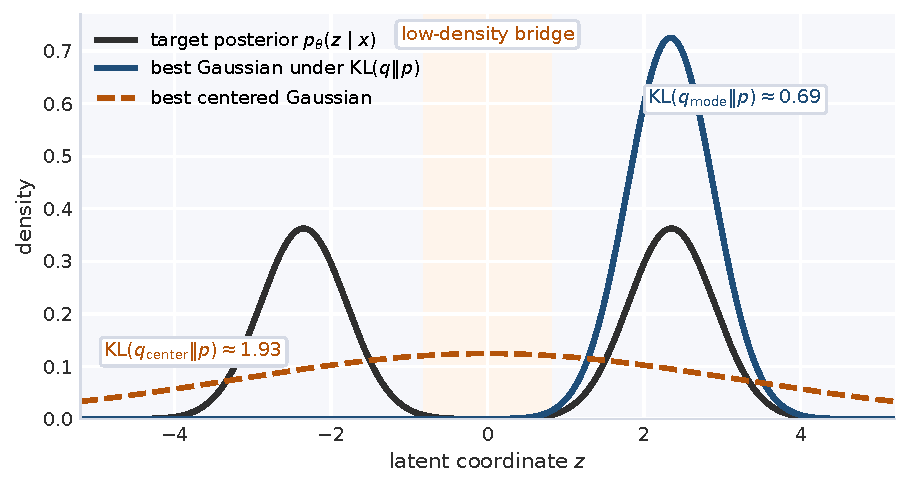
\includegraphics[width=0.92\linewidth]{figures/handouts/elbo_geometry/fig_forward_kl_undercoverage_applied}
  \caption{A bimodal target posterior is approximated by a single Gaussian family.
  The centered Gaussian must place mass in the low-density region between the modes, while the forward-KL minimizer instead concentrates near one mode.
  This is the mode-seeking geometry behind undercoverage.}
  \label{fig:forward-kl-undercoverage-applied}
\end{figure}

In \Cref{fig:forward-kl-undercoverage-applied}, the centered approximation pays for mass throughout the low-density region between the modes, while the forward-KL minimizer avoids that bill and settles on one plausible region.

\begin{exercise}[A three-cell proxy for forward-KL undercoverage]
\label{ex:forward-kl-undercovers}
Approximate a bimodal posterior by three disjoint regions:
\(L\) for the left mode, \(M\) for the low-density middle region, and \(R\) for the right mode.
Suppose
\[
  p(L)=0.49,
  \qquad
  p(M)=0.02,
  \qquad
  p(R)=0.49.
\]
Consider two candidate unimodal approximations:
\[
  q_{\mathrm{mid}}=(0.25,0.50,0.25),
  \qquad
  q_{\mathrm{left}}=(1,0,0),
\]
listed in the order \((L,M,R)\).
\begin{enumerate}[leftmargin=*]
  \item Compute
  \[
    \operatorname{KL}(q_{\mathrm{mid}}\|p)
    =
    \sum_{A\in\{L,M,R\}}
    q_{\mathrm{mid}}(A)\log\frac{q_{\mathrm{mid}}(A)}{p(A)}.
  \]
  \item Compute
  \[
    \operatorname{KL}(q_{\mathrm{left}}\|p).
  \]
  \item Which candidate is preferred by forward KL?
  Explain in one or two sentences which term in the objective makes the centered approximation expensive.
\end{enumerate}
\end{exercise}
\SolutionBox[12]{For the centered candidate,
\[
  \operatorname{KL}(q_{\mathrm{mid}}\|p)
  =
  0.25\log\frac{0.25}{0.49}
  +
  0.50\log\frac{0.50}{0.02}
  +
  0.25\log\frac{0.25}{0.49}
  =
  \frac12\log\frac{625}{49}.
\]
For the left-mode candidate,
\[
  \operatorname{KL}(q_{\mathrm{left}}\|p)
  =
  1\cdot \log\frac{1}{0.49}
  =
  \log\frac{100}{49}.
\]
Numerically,
\[
  \frac12\log\frac{625}{49}\approx 1.27,
  \qquad
  \log\frac{100}{49}\approx 0.71,
\]
so forward KL prefers \(q_{\mathrm{left}}\).
The key penalty is the middle-region term
\[
  0.50\log\frac{0.50}{0.02},
\]
which is large because the centered approximation places substantial mass where the target density is tiny.
This is the discrete version of undercoverage: missing one mode can be cheaper than paying for mass in a low-density middle region.}

The cleanest next example is mean-field VI, where the family deletes dependence before optimization ever starts.

\section{Mean-field deletes dependence before optimization starts}
\label{sec:mean-field-geometry}

\subsection{Factorization is the real approximation}
\label{subsec:mean-field-cavi}

Mean-field VI is the first place where the phrase ``the family is part of the model'' becomes concrete.
Write the latent variable as \(z=(z_1,\dots,z_m)\) and consider the factorized family
\[
  q(z)=\prod_{j=1}^m q_j(z_j).
\]
The point of this choice is not that coordinate ascent is especially deep.
The point is that the posterior is now allowed to move only inside a product geometry.
Any dependence in the true posterior has already been deleted before the optimizer gets to work.

\begin{proposition}[Mean-field coordinate update]
\label{prop:mean-field-update-handout}
Fix all factors except \(q_j\), and assume
\[
  m_j(z_j)\coloneqq \E_{q_{-j}}[\log p_\theta(x,z)]
\]
is finite almost everywhere with \(\int e^{m_j(z_j)}\,dz_j<\infty\).
Then any maximizer of the ELBO over the remaining factor satisfies
\[
  q_j^\star(z_j)
  \propto
  \exp\!\left(
    \E_{q_{-j}}\bigl[\log p_\theta(x,z)\bigr]
  \right),
\]
where the expectation is taken under the current variational law on the remaining coordinates.
\end{proposition}
\begin{proof}
Holding \(q_{-j}\) fixed and optimizing only over \(q_j\), the ELBO becomes
\[
  \mathcal{L}(q;x)
  =
  \int q_j(z_j)\,m_j(z_j)\,dz_j
  -
  \int q_j(z_j)\log q_j(z_j)\,dz_j
  + C,
\]
where \(C\) does not depend on \(q_j\).
Define
\[
  Z_j\coloneqq \int e^{m_j(u)}\,du,
  \qquad
  \widetilde q_j(z_j)\coloneqq Z_j^{-1}e^{m_j(z_j)}.
\]
Then
\[
  \mathcal{L}(q;x)
  =
  -\operatorname{KL}\!\bigl(q_j\,\|\,\widetilde q_j\bigr)+\log Z_j+C,
\]
so the ELBO is maximized at \(q_j=\widetilde q_j\).%
\end{proof}

This is the deterministic analogue of a Gibbs update:
instead of sampling one coordinate from an exact conditional, we replace one factor by the best ELBO fit given the others.
But the more important point is geometric.
Once the family has been factorized, CAVI can only repair the posterior inside that factorized geometry.

\begin{figure}[t]
  \centering
  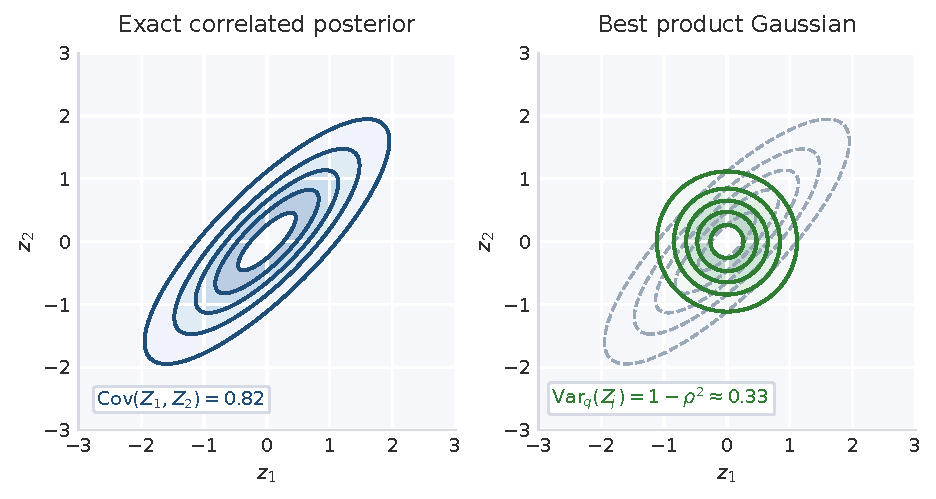
\includegraphics[width=0.92\linewidth]{figures/handouts/elbo_geometry/fig_mean_field_correlation_loss_applied}
  \caption{A correlated Gaussian posterior is compared with the best product Gaussian from the mean-field family.
  The surrogate removes the tilted covariance structure and shrinks each marginal variance, matching the analytic minimizer computed below.}
  \label{fig:mean-field-correlation-loss}
\end{figure}

That loss of geometry is not a training accident.
It is the structural cost of replacing a joint posterior by a product family.
\Cref{fig:mean-field-correlation-loss} shows the cleanest case:
the target posterior is as friendly as possible, but the family is not allowed to tilt.

\begin{proposition}[Best product-Gaussian fit to a correlated Gaussian]
\label{prop:mfvi-gaussian-underdispersion}
Let the exact posterior be
\[
  p_\theta(z\mid x)=\mathcal{N}(0,\Sigma_\rho),
  \qquad
  \Sigma_\rho=
  \begin{bmatrix}
    1 & \rho\\
    \rho & 1
  \end{bmatrix},
  \qquad
  0<|\rho|<1.
\]
Among all fully factorized Gaussian approximations
\[
  q(z_1,z_2)=\mathcal{N}(m_1,s_1^2)\,\mathcal{N}(m_2,s_2^2),
\]
the unique minimizer of
\(\operatorname{KL}(q(z_1,z_2)\|p_\theta(z\mid x))\) satisfies
\[
  m_1=m_2=0,
  \qquad
  s_1^2=s_2^2=1-\rho^2.
\]
In particular, the optimal mean-field approximation is not only uncorrelated; it is also under-dispersed in each coordinate whenever \(\rho\neq 0\).
\end{proposition}
\begin{proof}
The precision matrix is
\[
  \Sigma_\rho^{-1}
  =
  \frac{1}{1-\rho^2}
  \begin{bmatrix}
    1 & -\rho\\
    -\rho & 1
  \end{bmatrix}.
\]
A direct Gaussian-KL calculation gives
\[
  \operatorname{KL}(q\|p_\theta(\cdot\mid x))
  =
  \frac12\left[
    \frac{m_1^2-2\rho m_1m_2+m_2^2+s_1^2+s_2^2}{1-\rho^2}
    -2
    +
    \log\!\frac{1-\rho^2}{s_1^2s_2^2}
  \right].
\]
The quadratic form in \((m_1,m_2)\) is minimized uniquely at \(m_1=m_2=0\).
For \(j\in\{1,2\}\),
\[
  \frac{\partial}{\partial s_j^2}\operatorname{KL}(q\|p_\theta(\cdot\mid x))
  =
  \frac12\left(\frac{1}{1-\rho^2}-\frac{1}{s_j^2}\right),
\]
so the unique stationary point is \(s_j^2=1-\rho^2\).
Since the second derivative with respect to \(s_j^2\) is \(1/(2s_j^4)>0\), this stationary point is the global minimizer.%
\end{proof}

This calculation says exactly what the picture suggests.
The best product approximation cannot reproduce the tilted covariance geometry, so it compensates by shrinking the marginal variances.
Even in the Gaussian case, forward KL plus factorization produces an axis-aligned, overconfident surrogate.

\begin{exercise}[Recover the best product Gaussian]
\label{ex:mean-field-removes-dependence}
Use the displayed formula
\[
  \operatorname{KL}(q\|p_\theta(\cdot\mid x))
  =
  \frac12\left[
    \frac{m_1^2-2\rho m_1m_2+m_2^2+s_1^2+s_2^2}{1-\rho^2}
    -2
    +
    \log\!\frac{1-\rho^2}{s_1^2s_2^2}
  \right]
\]
for the factorized Gaussian \(q(z)=\mathcal{N}(m_1,s_1^2)\mathcal{N}(m_2,s_2^2)\).
\begin{enumerate}[leftmargin=*]
  \item Holding \(s_1^2,s_2^2\) fixed, differentiate with respect to \(m_1,m_2\) and show that the unique stationary point is \(m_1=m_2=0\).
  \item Differentiate with respect to \(s_1^2\) and \(s_2^2\) and show that the minimizer satisfies
  \[
    s_1^2=s_2^2=1-\rho^2.
  \]
  \item Compare these values with the exact posterior variances and covariance. What two geometric distortions does the best product approximation impose?
\end{enumerate}
\end{exercise}
\SolutionBox[12]{Differentiating the KL with respect to the means gives
\[
  \frac{\partial}{\partial m_1}\operatorname{KL}(q\|p_\theta(\cdot\mid x))
  =
  \frac{m_1-\rho m_2}{1-\rho^2},
  \qquad
  \frac{\partial}{\partial m_2}\operatorname{KL}(q\|p_\theta(\cdot\mid x))
  =
  \frac{m_2-\rho m_1}{1-\rho^2}.
\]
The stationary conditions are
\[
  m_1=\rho m_2,
  \qquad
  m_2=\rho m_1.
\]
Since \(|\rho|<1\), the unique solution is \(m_1=m_2=0\).
For the variances,
\[
  \frac{\partial}{\partial s_j^2}\operatorname{KL}(q\|p_\theta(\cdot\mid x))
  =
  \frac12\left(\frac{1}{1-\rho^2}-\frac{1}{s_j^2}\right),
  \qquad j\in\{1,2\},
\]
so the stationary point is \(s_1^2=s_2^2=1-\rho^2\), which is the minimizer.
The exact posterior has marginal variances \(1\) and covariance \(\rho\), while the best product approximation has variances \(1-\rho^2<1\) and covariance \(0\).
So mean-field imposes two distortions at once: it deletes posterior dependence and it shrinks each marginal variance below the true one.}

Up to this point every failure has been local:
one observation, one posterior, one restricted family.
Amortization adds a second restriction across data.

\section{Shared encoders and one latent bottleneck}
\label{sec:shared-encoder-bottleneck}

\subsection{Amortization adds a second restriction}
\label{subsec:amortization-gap}

Amortized VI replaces per-datum variational optimization by a shared encoder \(q_\phi(z\mid x)\).
That makes inference scalable, but it also means that all posterior approximations must lie on the image of one learned map \(x\mapsto q_\phi(\cdot\mid x)\).
On a data set \(x_1,\dots,x_n\), the optimization problem becomes
\[
  \max_{\phi\in\Phi}\sum_{i=1}^n \mathcal{L}(q_\phi(\cdot\mid x_i);x_i)
  \qquad\text{instead of}\qquad
  \sum_{i=1}^n \max_{q\in\mathcal{Q}} \mathcal{L}(q;x_i).
\]
So amortization is not just a faster optimizer for the same approximation problem.
It is a smaller approximation problem.

\begin{figure}[t]
  \centering
  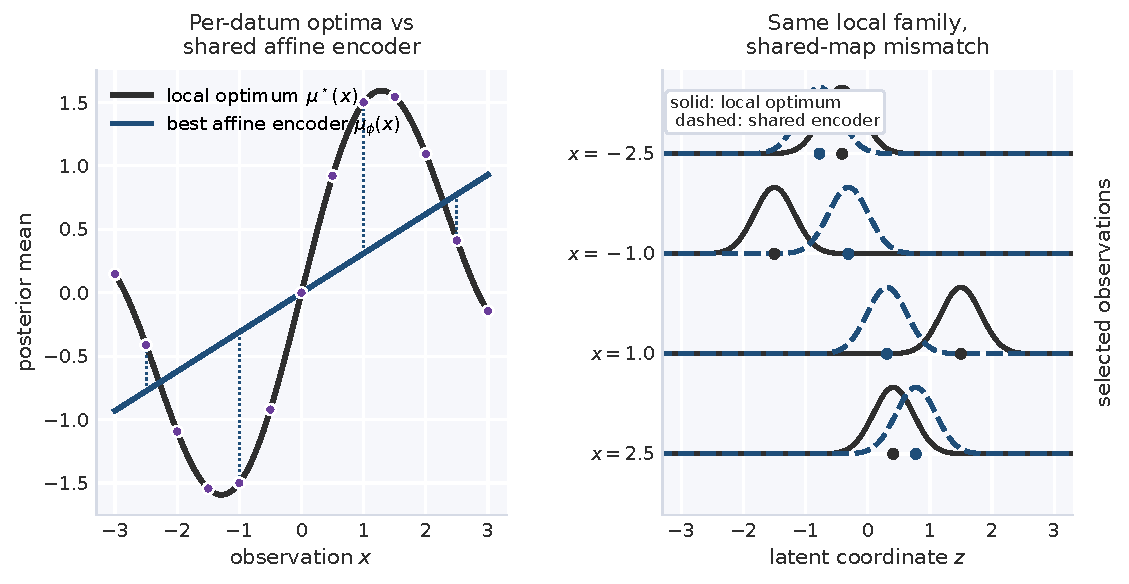
\includegraphics[width=\linewidth]{figures/handouts/elbo_geometry/fig_vi_amortization_applied}
  \caption{A synthetic posterior family with nonlinear per-datum optima \(\mu^\star(x)\) is approximated by a shared affine encoder family.
  The local posteriors are individually representable, but one shared map cannot hit all of the targets simultaneously.
  This is the amortization gap.}
  \label{fig:vi-amortization-handout}
\end{figure}

\Cref{fig:vi-amortization-handout} separates two failure modes that are easy to conflate.
The local family may be adequate for each datum, yet the shared encoder may still miss the local optimum because one map cannot bend in all the required directions at once.

\begin{proposition}[Amortization cannot beat per-datum variational optima]
\label{prop:amortization-gap}
Let \(x_1,\dots,x_n\) be observations, and let \(\mathcal{Q}\) be a variational family available for each datum individually.
Define
\[
  \mathcal{L}_i^\star \coloneqq \sup_{q\in\mathcal{Q}} \mathcal{L}(q;x_i).
\]
Then for any amortized family \(\{q_\phi(\cdot\mid x):\phi\in\Phi\}\subseteq \mathcal{Q}\),
\[
  \sup_{\phi\in\Phi} \sum_{i=1}^n \mathcal{L}(q_\phi(\cdot\mid x_i);x_i)
  \le
  \sum_{i=1}^n \mathcal{L}_i^\star.
\]
\end{proposition}
\begin{proof}
Fix \(\phi\).
For each \(i\), the distribution \(q_\phi(\cdot\mid x_i)\) belongs to \(\mathcal{Q}\), so
\[
  \mathcal{L}(q_\phi(\cdot\mid x_i);x_i)\le \mathcal{L}_i^\star.
\]
Summing over \(i\) gives
\[
  \sum_{i=1}^n \mathcal{L}(q_\phi(\cdot\mid x_i);x_i)\le \sum_{i=1}^n \mathcal{L}_i^\star.
\]
Taking the supremum over \(\phi\) preserves the inequality.%
\end{proof}

The proposition is simple, but it is the correct formal separation between family mismatch and amortization gap.
The gap vanishes only if one shared encoder hits the per-datum optimum everywhere.
Computationally, amortization is still the right idea:
the recognition model and the reparameterized gradient estimator from AEVB and stochastic backpropagation make \(\mathcal{J}(\theta,\phi)\) trainable at scale
\citep[\S\S2.1--2.3]{kingma_welling_2014_aevb}
\citep[\S\S1, 3]{rezende_mohamed_wierstra_2014_stochastic_backpropagation}.
But neither device removes the underlying geometric restriction.

\begin{exercise}[Decompose local mismatch and amortization gap]
\label{ex:amortization-gap}
Let
\[
  \mathcal{L}_i^\star
  \coloneqq
  \sup_{q\in\mathcal{Q}}\mathcal{L}(q;x_i),
  \qquad i=1,\dots,n.
\]
Define the local approximation gap
\[
  \Delta_i^{\mathrm{loc}}
  \coloneqq
  \log p_\theta(x_i)-\mathcal{L}_i^\star
\]
and the amortization gap
\[
  \Delta_{\mathrm{am}}
  \coloneqq
  \sum_{i=1}^n \mathcal{L}_i^\star
  -
  \sup_{\phi\in\Phi}\sum_{i=1}^n \mathcal{L}(q_\phi(\cdot\mid x_i);x_i).
\]
Assume the amortized family satisfies
\[
  \{q_\phi(\cdot\mid x_i):\phi\in\Phi\}\subseteq \mathcal{Q}
  \qquad\text{for every }i.
\]
\begin{enumerate}[leftmargin=*]
  \item Use the ELBO--KL identity to show that, for each \(i\),
  \[
    \Delta_i^{\mathrm{loc}}
    =
    \inf_{q\in\mathcal{Q}}
    \operatorname{KL}\!\bigl(q(z)\,\|\,p_\theta(z\mid x_i)\bigr),
  \]
  and in particular \(\Delta_i^{\mathrm{loc}}\ge 0\).
  \item Use \Cref{prop:amortization-gap} to show \(\Delta_{\mathrm{am}}\ge 0\).
  \item Fix \(\phi\). Show that for each \(i\),
  \[
    \mathcal{L}(q_\phi(\cdot\mid x_i);x_i)\le \mathcal{L}_i^\star.
  \]
  Then sum over \(i\) and take the supremum over \(\phi\) to recover the inequality
  \[
    \sup_{\phi\in\Phi}\sum_{i=1}^n \mathcal{L}(q_\phi(\cdot\mid x_i);x_i)
    \le
    \sum_{i=1}^n \mathcal{L}_i^\star.
  \]
  \item Prove the exact decomposition
  \[
    \sum_{i=1}^n \log p_\theta(x_i)
    -
    \sup_{\phi\in\Phi}\sum_{i=1}^n \mathcal{L}(q_\phi(\cdot\mid x_i);x_i)
    =
    \sum_{i=1}^n \Delta_i^{\mathrm{loc}}
    +
    \Delta_{\mathrm{am}}.
  \]
  \item Explain what vanishes in the two extreme cases:
  a purely local-family-limited regime and a purely amortization-limited regime.
\end{enumerate}
\end{exercise}
\SolutionBox[15]{By the ELBO--KL identity,
\[
  \log p_\theta(x_i)
  =
  \mathcal{L}(q;x_i)
  +
  \operatorname{KL}\!\bigl(q(z)\,\|\,p_\theta(z\mid x_i)\bigr)
\]
for every admissible \(q\in\mathcal{Q}\).
Taking the supremum over \(q\in\mathcal{Q}\) on the ELBO side is the same as taking the infimum of the KL term, so
\[
  \Delta_i^{\mathrm{loc}}
  =
  \log p_\theta(x_i)-\mathcal{L}_i^\star
  =
  \inf_{q\in\mathcal{Q}}
  \operatorname{KL}\!\bigl(q(z)\,\|\,p_\theta(z\mid x_i)\bigr)\ge 0.
\]
Next,
\[
  \Delta_{\mathrm{am}}
  =
  \sum_{i=1}^n \mathcal{L}_i^\star
  -
  \sup_{\phi\in\Phi}\sum_{i=1}^n \mathcal{L}(q_\phi(\cdot\mid x_i);x_i)\ge 0
\]
by \Cref{prop:amortization-gap}.
Fix \(\phi\).
For each datum \(x_i\), the distribution \(q_\phi(\cdot\mid x_i)\) belongs to \(\mathcal{Q}\), so by definition of \(\mathcal{L}_i^\star\),
\[
  \mathcal{L}(q_\phi(\cdot\mid x_i);x_i)\le \mathcal{L}_i^\star.
\]
Summing over \(i\) gives
\[
  \sum_{i=1}^n \mathcal{L}(q_\phi(\cdot\mid x_i);x_i)
  \le
  \sum_{i=1}^n \mathcal{L}_i^\star.
\]
Taking the supremum over \(\phi\) preserves the inequality and yields the claim.
For the exact decomposition, add and subtract \(\sum_i \mathcal{L}_i^\star\):
\begin{align*}
  \sum_{i=1}^n \log p_\theta(x_i)
  -
  \sup_{\phi}\sum_{i=1}^n \mathcal{L}(q_\phi(\cdot\mid x_i);x_i)
  &=
  \sum_{i=1}^n \bigl(\log p_\theta(x_i)-\mathcal{L}_i^\star\bigr) \\
  &\quad
  +
  \sum_{i=1}^n \mathcal{L}_i^\star
  -
  \sup_{\phi}\sum_{i=1}^n \mathcal{L}(q_\phi(\cdot\mid x_i);x_i) \\
  &=
  \sum_{i=1}^n \Delta_i^{\mathrm{loc}}+\Delta_{\mathrm{am}}.
\end{align*}
In a purely local-family-limited regime, \(\Delta_{\mathrm{am}}=0\) and the whole gap comes from the local family \(\mathcal{Q}\) being too small.
In a purely amortization-limited regime, every \(\Delta_i^{\mathrm{loc}}=0\) and the whole gap comes from one shared encoder failing to realize the per-datum optima.}

\subsection{Blur: overlapping latent neighborhoods force averaging}
\label{subsec:blur}

From this point on, keep the standard one-bottleneck VAE in mind:
a prior \(p(z)\), decoder \(p_\theta(x\mid z)\), and shared encoder \(q_\phi(z\mid x)\).
This is the AEVB setting with the usual reparameterization
\[
  z=\mu_\phi(x)+\sigma_\phi(x)\odot \varepsilon,
  \qquad
  \varepsilon\sim\mathcal{N}(0,I),
\]
which makes stochastic ELBO optimization practical but does not alter the geometry of the approximation problem
\citep[\S\S2.1--2.3]{kingma_welling_2014_aevb}
\citep[\S3]{rezende_mohamed_wierstra_2014_stochastic_backpropagation}.

The blur mechanism becomes sharp when the decoder is Gaussian.
Then, for fixed \(q_\phi\), decoder learning is literally a regression problem under the joint law induced by the data and the encoder.
That is the direct link from ``posterior overlap'' to blurry reconstructions.

\begin{proposition}[A fixed-encoder Gaussian VAE is regression under \(p_{\mathrm{data}}(x)q_\phi(z\mid x)\)]
\label{prop:gaussian-vae-regression}
Assume \(\sigma^2>0\) is fixed and
\[
  p_\theta(x\mid z)=\mathcal{N}\!\bigl(\mu_\theta(z),\sigma^2 I\bigr).
\]
Then the expected ELBO over the data distribution satisfies
\[
  \E_{p_{\mathrm{data}}(x)}\!\bigl[\mathcal{L}(q_\phi;x)\bigr]
  =
  C(\phi,\sigma^2)
  -
  \frac{1}{2\sigma^2}
  \E_{(X,Z)\sim \pi_\phi}\!\bigl[\norm{X-\mu_\theta(Z)}_2^2\bigr],
\]
where
\[
  \pi_\phi(dx,dz)\coloneqq p_{\mathrm{data}}(x)\,q_\phi(dz\mid x)
\]
and
\[
  C(\phi,\sigma^2)
  =
  -\frac{d}{2}\log(2\pi\sigma^2)
  -
  \E_{p_{\mathrm{data}}(x)}
  \operatorname{KL}\!\bigl(q_\phi(z\mid x)\,\|\,p(z)\bigr)
\]
does not depend on \(\mu_\theta\).
Consequently, for fixed \(q_\phi\), maximizing the expected ELBO over decoder means \(\mu_\theta\) is equivalent to minimizing
\[
  \mu\mapsto
  \E_{(X,Z)\sim \pi_\phi}\!\bigl[\norm{X-\mu(Z)}_2^2\bigr].
\]
\end{proposition}
\begin{proof}
For each \(x\),
\[
  \mathcal{L}(q_\phi;x)
  =
  \E_{q_\phi(z\mid x)}[\log p_\theta(x\mid z)]
  -
  \operatorname{KL}\!\bigl(q_\phi(z\mid x)\,\|\,p(z)\bigr).
\]
Under the Gaussian decoder,
\[
  \log p_\theta(x\mid z)
  =
  -\frac{d}{2}\log(2\pi\sigma^2)
  -
  \frac{1}{2\sigma^2}\norm{x-\mu_\theta(z)}_2^2.
\]
Taking expectations over \(p_{\mathrm{data}}(x)\) gives
\begin{align*}
  \E_{p_{\mathrm{data}}(x)}\!\bigl[\mathcal{L}(q_\phi;x)\bigr]
  &=
  -\frac{d}{2}\log(2\pi\sigma^2)
  -
  \frac{1}{2\sigma^2}
  \E_{p_{\mathrm{data}}(x)q_\phi(z\mid x)}
  \norm{x-\mu_\theta(z)}_2^2 \\
  &\quad
  -
  \E_{p_{\mathrm{data}}(x)}
  \operatorname{KL}\!\bigl(q_\phi(z\mid x)\,\|\,p(z)\bigr),
\end{align*}
which is the stated identity.%
\end{proof}

\begin{proposition}[Squared loss chooses conditional means]
\label{prop:squared-error-mean}
Let \((X,Z)\) be jointly distributed with \(X\in\R^d\), \(Z\in\R^m\), and \(\E\norm{X}_2^2<\infty\).
Among all measurable maps \(\mu:\R^m\to\R^d\) such that \(\E\norm{\mu(Z)}_2^2<\infty\), the minimizer of
\[
  \mu\mapsto \E\norm{X-\mu(Z)}_2^2
\]
satisfies
\[
  \mu^\star(Z)=\E[X\mid Z]
\]
almost surely, where \(\E[X\mid Z]\) denotes any version of the conditional expectation.
\end{proposition}
\begin{proof}
For any measurable \(\mu\),
\begin{align*}
  \E\norm{X-\mu(Z)}_2^2
  &=
  \E\norm{X-\E[X\mid Z]}_2^2
  +
  \E\norm{\E[X\mid Z]-\mu(Z)}_2^2 \\
  &\quad
  +
  2\,\E\!\left[
    \ip{X-\E[X\mid Z]}{\E[X\mid Z]-\mu(Z)}
  \right].
\end{align*}
The cross term vanishes because
\[
  \E\!\left[X-\E[X\mid Z]\mid Z\right]=0
\]
and \(\E[X\mid Z]-\mu(Z)\) is \(Z\)-measurable.
Therefore
\[
  \E\norm{X-\mu(Z)}_2^2
  =
  \E\norm{X-\E[X\mid Z]}_2^2
  +
  \E\norm{\E[X\mid Z]-\mu(Z)}_2^2,
\]
so the minimum is attained exactly when \(\mu(Z)=\E[X\mid Z]\) almost surely.%
\end{proof}

\Cref{prop:gaussian-vae-regression} and \Cref{prop:squared-error-mean} give the blur mechanism in one line:
for fixed \(q_\phi\), a Gaussian decoder mean that minimizes the reconstruction risk is any version of
\[
  \mu_\theta^\star(Z)=\E_{\pi_\phi}[X\mid Z]
\]
almost surely.
So if the encoder geometry pushes several incompatible observations into the same latent neighborhood, the decoder is forced toward a conditional mean rather than any one sharp sample.
This makes precise the ``posterior overlap'' and ``locality'' story emphasized in the \(\beta\)-VAE discussion of \citet[\S\S4.2--5]{burgess_higgins_pal_matthey_watters_desjardins_lerchner_2018_understanding_bvae}.

\subsubsection{A two-point blur example}
\label{subsubsec:two-point-blur}

The abstract conditional-mean statement becomes concrete in the smallest nontrivial example.
If one latent neighborhood mixes two genuinely different observations, the decoder has no sharper target available than their average.

\begin{example}[Ambiguity forces averaging]
\label{ex:two-point-blur}
Suppose the data distribution places probability \(1/2\) on \(x^{(1)}\in\R^d\) and probability \(1/2\) on \(x^{(2)}\in\R^d\), and suppose that a version of the conditional law of \(X\) given \(Z\) satisfies, at some latent location \(z\),
\[
  \Pr(X=x^{(1)}\mid Z=z)
  =
  \Pr(X=x^{(2)}\mid Z=z)
  =
  \frac12.
\]
Then a risk-minimizing Gaussian-decoder prediction at that latent point is
\[
  \mu_\theta(z)
  =
  \E[X\mid Z=z]
  =
  \frac{x^{(1)}+x^{(2)}}{2}.
\]
Unless \(x^{(1)}=x^{(2)}\), the reconstruction is an average rather than an actual datum.
\end{example}

The example is tiny, but it captures the full story.
Blur does not mean the decoder is inherently bad at detail.
It means the encoder geometry failed to separate distinctions that matter to squared-error reconstruction.
When the bottleneck has too little effective capacity, the decoder is rewarded for averaging unresolved variation
\citep[\S\S4.2--5]{burgess_higgins_pal_matthey_watters_desjardins_lerchner_2018_understanding_bvae}.

\begin{figure}[t]
  \centering
  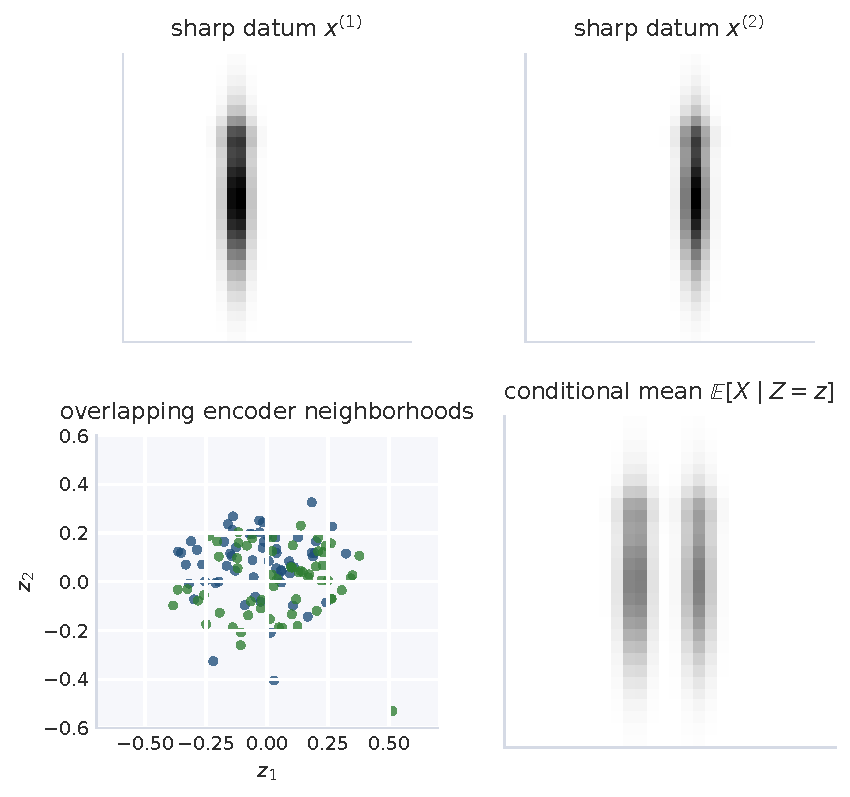
\includegraphics[width=0.84\linewidth]{figures/handouts/elbo_geometry/fig_latent_overlap_blur_applied}
  \caption{Two distinct sharp observations are mapped into nearly the same latent neighborhood.
  A Gaussian decoder therefore returns their conditional mean, which is visibly blurrier than either endpoint.}
  \label{fig:latent-overlap-blur}
\end{figure}

\begin{exercise}[The irreducible blur penalty]
\label{ex:blur-average}
In the two-point example above, show the exact identity
\[
  \frac12\norm{x^{(1)}-a}_2^2+\frac12\norm{x^{(2)}-a}_2^2
  =
  \frac14\norm{x^{(1)}-x^{(2)}}_2^2
  +
  \norm{a-\tfrac12(x^{(1)}+x^{(2)})}_2^2.
\]
Deduce that the minimizer is \(a=(x^{(1)}+x^{(2)})/2\) and compute the minimum value explicitly in terms of \(\norm{x^{(1)}-x^{(2)}}_2\).
Then explain how this finite identity mirrors the decomposition in \Cref{prop:squared-error-mean}.
\end{exercise}
\SolutionBox[9]{Expanding the quadratic gives
\[
  \frac12\norm{x^{(1)}-a}_2^2+\frac12\norm{x^{(2)}-a}_2^2
  =
  \frac14\norm{x^{(1)}-x^{(2)}}_2^2
  +
  \norm{a-\tfrac12(x^{(1)}+x^{(2)})}_2^2.
\]
Hence the minimizer is the midpoint \(a=(x^{(1)}+x^{(2)})/2\).
The minimum value is
\[
  \frac14\norm{x^{(1)}-x^{(2)}}_2^2.
\]
This is the two-point version of \Cref{prop:squared-error-mean}: the first term is the irreducible conditional-variance cost, and the second term is the extra penalty for choosing a prediction different from the conditional mean.
So even the best decoder incurs a positive reconstruction penalty whenever distinct observations share one latent code.}

\subsection{Collapse: the decoder can make latent information too expensive}
\label{subsec:collapse}

Blur and collapse are opposite-looking symptoms of the same bottleneck picture.
In blur, the latent code is used but is not expressive enough to separate incompatible observations.
In collapse, the decoder becomes so strong that using \(z\) is not worth the KL bill.
The cleanest formal toy case is when the decoder literally ignores \(z\).

\begin{proposition}[If the decoder ignores \(z\), the ELBO prefers the prior]
\label{prop:collapse-if-decoder-ignores-z}
Suppose \(p_\theta(x\mid z)=p_\theta(x)\) for all \(z\).
Then for every \(x\),
\[
  \mathcal{L}(q;x)=\log p_\theta(x)-\operatorname{KL}\!\bigl(q(z)\,\|\,p(z)\bigr),
\]
so the ELBO is maximized by \(q(z)=p(z)\).
\end{proposition}
\begin{proof}
Under the assumption \(p_\theta(x\mid z)=p_\theta(x)\),
\[
  p_\theta(x,z)=p_\theta(x)\,p(z).
\]
Substituting this into the ELBO gives
\[
  \mathcal{L}(q;x)
  =
  \E_q[\log p_\theta(x)+\log p(z)-\log q(z)]
  =
  \log p_\theta(x)-\operatorname{KL}\!\bigl(q(z)\,\|\,p(z)\bigr).
\]
The KL term is minimized at \(q(z)=p(z)\), proving the claim.%
\end{proof}

Real posterior collapse is usually less extreme than this toy case, but the geometry is the same.
If the decoder can already explain \(x\) well enough on its own, then the ELBO charges for transmitting information through \(z\) without demanding much in return.
The latent variable becomes expendable.

To see the bill more clearly, average the KL term over the data distribution and define the aggregate posterior
\[
  q_\phi(z)
  \coloneqq
  \int q_\phi(z\mid x)\,p_{\mathrm{data}}(x)\,dx.
\]

\begin{proposition}[Mutual-information decomposition of the KL term]
\label{prop:mi-decomposition}
Assume \(q_\phi(z\mid x)\) and \(p(z)\) are densities with respect to a common base measure and that the displayed expectations are finite.
We have
\[
  \E_{p_{\mathrm{data}}(x)}
  \operatorname{KL}\!\bigl(q_\phi(z\mid x)\,\|\,p(z)\bigr)
  =
  I_q(X;Z)
  +
  \operatorname{KL}\!\bigl(q_\phi(z)\,\|\,p(z)\bigr),
\]
where \(I_q(X;Z)\) is mutual information under the joint law
\[
  p_{\mathrm{data}}(x)\,q_\phi(z\mid x).
\]
\end{proposition}
\begin{proof}
Expand the left-hand side:
\[
  \E_{p_{\mathrm{data}}(x)q_\phi(z\mid x)}
  \bigl[\log q_\phi(z\mid x)-\log p(z)\bigr].
\]
Add and subtract \(\log q_\phi(z)\):
\[
  \E\!\bigl[\log q_\phi(z\mid x)-\log q_\phi(z)\bigr]
  +
  \E\!\bigl[\log q_\phi(z)-\log p(z)\bigr].
\]
The first term is \(I_q(X;Z)\), and the second is
\(\operatorname{KL}(q_\phi(z)\|p(z))\).%
\end{proof}

Combining \Cref{prop:mi-decomposition} with the expected ELBO gives
\[
  \E_{p_{\mathrm{data}}(x)}\!\bigl[\mathcal{L}(q_\phi;x)\bigr]
  =
  \E_{p_{\mathrm{data}}(x)q_\phi(z\mid x)}[\log p_\theta(x\mid z)]
  -
  I_q(X;Z)
  -
  \operatorname{KL}\!\bigl(q_\phi(z)\,\|\,p(z)\bigr).
\]
So the KL regularizer is charging for two things at once:
how much information the code stores about the data, and how far the aggregate code distribution drifts from the prior.
If the decoder class already contains good nearly unconditional models for the data, the collapsed solution can be globally competitive; more generally, using \(z\) is worthwhile only when the reconstruction gain beats this information bill.

This helps explain why expressive autoregressive decoders often collapse in practice.
Bowman et al.\ show the sentence-VAE version of this story:
if the decoder is already a strong language model, training pushes \(q_\phi(z\mid x)\) back toward the prior unless the optimization pressure is modified
\citep[\S3.1]{bowman_vilnis_vinyals_dai_jozefowicz_bengio_2016_generating_sentences}.
He et al.\ give the complementary dynamic explanation:
early in training the decoder can move faster than the inference network, and that lag can steer the system into a collapsed regime before the encoder learns to use \(z\)
\citep[\S\S3--4]{he_spokoyny_neubig_bergkirkpatrick_2019_lagging_inference}.

\begin{figure}[t]
  \centering
  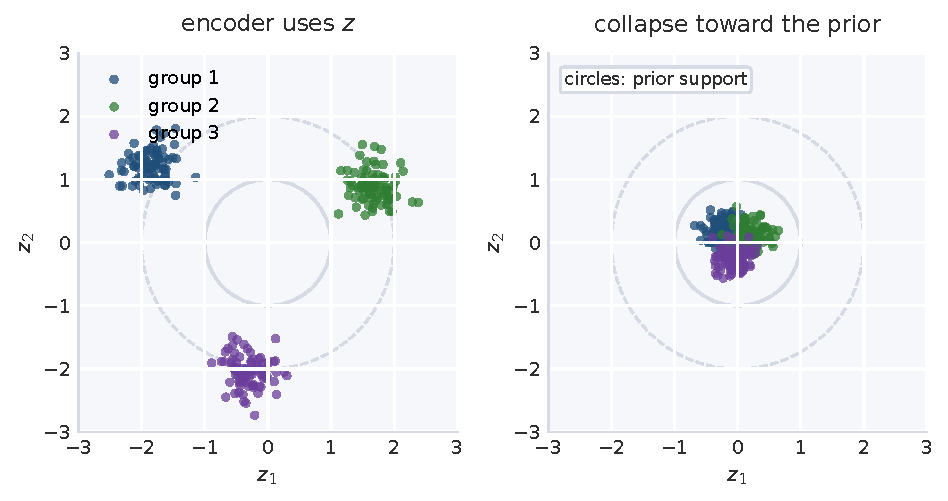
\includegraphics[width=0.90\linewidth]{figures/handouts/elbo_geometry/fig_decoder_bypass_collapse_applied}
  \caption{Toy encoder outputs for three groups of observations.
  When the latent variable is used, the group-conditioned posteriors separate in latent space; under posterior collapse they contract back toward the prior and overlap heavily, so little information about \(x\) remains in \(z\).}
  \label{fig:decoder-bypass-collapse}
\end{figure}

This also clarifies what KL warm-up and \(\beta\)-VAE style heuristics do.
They change the price of information.
That can change which local optimum training reaches, but it does not enlarge the variational family or remove the possibility of collapse
\citep[\S3.1]{bowman_vilnis_vinyals_dai_jozefowicz_bengio_2016_generating_sentences}
\citep[\S\S3--5]{burgess_higgins_pal_matthey_watters_desjardins_lerchner_2018_understanding_bvae}.

\begin{exercise}[\(\beta\)-ELBO as a weighted information budget]
\label{ex:beta-elbo}
Consider the \(\beta\)-ELBO
\[
  \mathcal{L}_\beta(q;x)
  =
  \E_q[\log p_\theta(x\mid z)]
  -
  \beta\,\operatorname{KL}\!\bigl(q(z)\,\|\,p(z)\bigr).
\]
\begin{enumerate}[leftmargin=*]
  \item After averaging over \(p_{\mathrm{data}}(x)\), write the objective as
  \[
    \E_{p_{\mathrm{data}}(x)q_\phi(z\mid x)}[\log p_\theta(x\mid z)]
    -
    \beta\,\E_{p_{\mathrm{data}}(x)}
    \operatorname{KL}\!\bigl(q_\phi(z\mid x)\,\|\,p(z)\bigr).
  \]
  \item In the averaged KL term, add and subtract \(\log q_\phi(z)\) exactly as in the proof of \Cref{prop:mi-decomposition}.
  \item Identify the two resulting terms and conclude that
  \[
    \E_{p_{\mathrm{data}}(x)}[\mathcal{L}_\beta(q_\phi;x)]
    =
    \E_{p_{\mathrm{data}}(x)q_\phi(z\mid x)}[\log p_\theta(x\mid z)]
    -
    \beta\,I_q(X;Z)
    -
    \beta\,\operatorname{KL}\!\bigl(q_\phi(z)\,\|\,p(z)\bigr).
  \]
  \item State separately what large \(\beta\) and small \(\beta\) do to the two non-reconstruction terms.
\end{enumerate}
\end{exercise}
\SolutionBox[10]{Apply \Cref{prop:mi-decomposition} to the averaged KL term:
\[
  \E_{p_{\mathrm{data}}(x)}
  \operatorname{KL}\!\bigl(q_\phi(z\mid x)\,\|\,p(z)\bigr)
  =
  I_q(X;Z)
  +
  \operatorname{KL}\!\bigl(q_\phi(z)\,\|\,p(z)\bigr).
\]
More explicitly,
\[
  \E\!\bigl[\log q_\phi(z\mid x)-\log p(z)\bigr]
  =
  \E\!\bigl[\log q_\phi(z\mid x)-\log q_\phi(z)\bigr]
  +
  \E\!\bigl[\log q_\phi(z)-\log p(z)\bigr],
\]
where the first expectation is \(I_q(X;Z)\) and the second is
\(\operatorname{KL}(q_\phi(z)\|p(z))\).
Substituting into the expected \(\beta\)-ELBO yields
\[
  \E_{p_{\mathrm{data}}(x)}[\mathcal{L}_\beta(q_\phi;x)]
  =
  \E_{p_{\mathrm{data}}(x)q_\phi(z\mid x)}[\log p_\theta(x\mid z)]
  -
  \beta\,I_q(X;Z)
  -
  \beta\,\operatorname{KL}\!\bigl(q_\phi(z)\,\|\,p(z)\bigr).
\]
So \(\beta\) directly rescales both parts of the KL bill.
Large \(\beta\) makes informative codes and prior mismatch expensive, which pushes toward weaker latent usage and can favor collapse.
Small \(\beta\) relaxes both penalties, so the model is more willing to store information in \(z\) and to let the aggregate posterior drift from the prior.
This changes optimization pressure, but it does not enlarge the family \(q_\phi(z\mid x)\), so it does not remove the underlying geometric mismatch.}

\section{Structural redesigns}
\label{sec:structural-redesigns}

Once the problem is framed this way, the right fix is often not ``optimize the same ELBO harder''.
If one latent layer is too coarse, or if learning the encoder geometry itself is unstable, then the approximation problem must change.
Two recurring redesigns do that:
hierarchy and fixed-bridge latent models.

\subsection{Hierarchy splits one overloaded KL bill into local bills}
\label{subsec:hierarchy-redistributes-kl}

A hierarchical VAE replaces one bottleneck by a stack of latent variables.
The key point is not just that the network is deeper.
The important change is that no single latent variable has to pay for every kind of variation at once.
Coarse structure can be represented high in the hierarchy and local detail lower down, so the ELBO decomposes into several local KL penalties instead of one global bottleneck charge.

Consider a hierarchical VAE with latent variables \(z_{1:L}\) and factorization
\[
  p_\theta(x,z_{1:L})
  =
  p_\theta(x\mid z_1)\,
  \prod_{\ell=1}^{L-1} p_\theta(z_\ell\mid z_{\ell+1})\,
  p(z_L),
\]
together with a structured encoder
\[
  q_\phi(z_{1:L}\mid x)
  =
  q_\phi(z_L\mid x)\,
  \prod_{\ell=1}^{L-1} q_\phi(z_\ell\mid z_{\ell+1},x).
\]

\begin{proposition}[Hierarchical ELBO as reconstruction minus local KL terms]
\label{prop:hierarchical-elbo}
For the model and encoder above,
\begin{align*}
  \mathcal{L}(q_\phi;x)
  &=
  \E_{q_\phi}\bigl[\log p_\theta(x\mid z_1)\bigr]
  -
  \operatorname{KL}\!\bigl(q_\phi(z_L\mid x)\,\|\,p(z_L)\bigr) \\
  &\quad
  -
  \sum_{\ell=1}^{L-1}
  \E_{q_\phi(z_{\ell+1:L}\mid x)}\!\left[
    \operatorname{KL}\!\bigl(
      q_\phi(z_\ell\mid z_{\ell+1},x)\,\|\,p_\theta(z_\ell\mid z_{\ell+1})
    \bigr)
  \right].
\end{align*}
\end{proposition}
\begin{proof}
Start from
\[
  \mathcal{L}(q_\phi;x)
  =
  \E_{q_\phi}\!\bigl[\log p_\theta(x,z_{1:L})-\log q_\phi(z_{1:L}\mid x)\bigr].
\]
Substituting the factorizations of \(p_\theta\) and \(q_\phi\) gives
\begin{align*}
  \mathcal{L}(q_\phi;x)
  &=
  \E_{q_\phi}[\log p_\theta(x\mid z_1)] \\
  &\quad
  +
  \E_{q_\phi}\!\left[
    \sum_{\ell=1}^{L-1} \log p_\theta(z_\ell\mid z_{\ell+1})
    + \log p(z_L)
    - \sum_{\ell=1}^{L-1} \log q_\phi(z_\ell\mid z_{\ell+1},x)
    - \log q_\phi(z_L\mid x)
  \right].
\end{align*}
The top-level terms combine as
\[
  \E_{q_\phi}\!\left[\log p(z_L)-\log q_\phi(z_L\mid x)\right]
  =
  -\operatorname{KL}\!\bigl(q_\phi(z_L\mid x)\,\|\,p(z_L)\bigr).
\]
For each \(\ell\in\{1,\dots,L-1\}\),
\begin{align*}
  &\E_{q_\phi}\!\left[
    \log p_\theta(z_\ell\mid z_{\ell+1})
    -
    \log q_\phi(z_\ell\mid z_{\ell+1},x)
  \right] \\
  &\qquad
  =
  -\E_{q_\phi(z_{\ell+1:L}\mid x)}\!\left[
    \operatorname{KL}\!\bigl(
      q_\phi(z_\ell\mid z_{\ell+1},x)\,\|\,p_\theta(z_\ell\mid z_{\ell+1})
    \bigr)
  \right].
\end{align*}
Substituting these identities back into the ELBO gives the result.%
\end{proof}

\Cref{prop:hierarchical-elbo} is the structural point in formula form.
The ELBO no longer contains one global penalty that forces a single latent variable to trade off every kind of information simultaneously.
Instead it contains a top-level prior-matching term and a sum of local conditional KL penalties.
That is why hierarchy can relieve both blur and collapse:
different scales of variation can be distributed across levels rather than compressed through one code.
This is exactly the design philosophy behind deep hierarchical VAEs such as NVAE, where global structure is represented high in the hierarchy and local detail is refined lower down
\citep[\S3.1]{vahdat_kautz_2020_nvae}.

\begin{figure}[t]
  \centering
  \begin{tikzpicture}[>=Stealth,font=\footnotesize]
  \tikzset{
    elbopanel/.style={
      draw=stat221Gray!30,
      fill=white,
      rounded corners=5pt,
      line width=0.6pt
    },
    elbotitle/.style={font=\small\bfseries, text=stat221Gray!90},
    latbox/.style={
      rounded corners=3pt,
      minimum width=1.95cm,
      minimum height=0.76cm,
      line width=0.8pt
    },
    elbobadge/.style={
      rounded corners=2pt,
      inner sep=2.6pt,
      font=\footnotesize,
      align=center,
      text=stat221Gray!85
    }
  }
  \path[use as bounding box] (-0.15,-0.24) rectangle (13.45,5.15);

  \node[elbopanel,minimum width=4.10cm,minimum height=4.95cm,anchor=north west] (leftpanel) at (0.0,4.85) {};
  \node[elbopanel,minimum width=4.10cm,minimum height=4.95cm,anchor=north west] (midpanel) at (4.62,4.85) {};
  \node[elbopanel,minimum width=4.10cm,minimum height=4.95cm,anchor=north west] (rightpanel) at (9.24,4.85) {};

  \node[elbotitle,anchor=north west] at ([xshift=0.25cm,yshift=-0.28cm]leftpanel.north west) {Single bottleneck};
  \node[elbotitle,anchor=north west] at ([xshift=0.25cm,yshift=-0.28cm]midpanel.north west) {Hierarchy splits scales};
  \node[elbotitle,anchor=north west] at ([xshift=0.25cm,yshift=-0.28cm]rightpanel.north west) {Cleaner allocation};

  \node[latbox,draw=stat221Purple!72!black,fill=stat221PurpleLight,minimum width=1.18cm,minimum height=0.68cm] (coarse) at (0.95,3.15) {class};
  \node[latbox,draw=stat221Blue!72!black,fill=stat221BlueLight,minimum width=1.28cm,minimum height=0.68cm] (detail) at (2.05,3.15) {detail};
  \node[latbox,draw=stat221Orange!78!black,fill=stat221OrangeLight,minimum width=1.22cm,minimum height=0.68cm] (noise) at (3.15,3.15) {noise};
  \node[latbox,draw=stat221Purple!72!black,fill=stat221PurpleLight,minimum width=2.15cm,minimum height=0.88cm] (z) at (2.05,1.95) {$z$};
  \node[latbox,draw=stat221Green!68!black,fill=stat221GreenLight,minimum width=2.15cm,minimum height=0.88cm] (x) at (2.05,0.75) {$x$};
  \draw[->,stat221Gray!75,line width=0.85pt] (coarse.south) -- (z.north west);
  \draw[->,stat221Gray!75,line width=0.85pt] (detail.south) -- (z.north);
  \draw[->,stat221Gray!75,line width=0.85pt] (noise.south) -- (z.north east);
  \draw[->,stat221Gray!75,line width=0.85pt] (z) -- (x);
  \node[elbobadge,fill=stat221Gray!8,anchor=west] at (2.72,1.30) {one KL budget};

  \node[latbox,draw=stat221Purple!72!black,fill=stat221PurpleLight,minimum width=2.05cm,minimum height=0.88cm] (z2) at (6.68,3.05) {$z_2$};
  \node[latbox,draw=stat221Blue!72!black,fill=stat221BlueLight,minimum width=2.05cm,minimum height=0.88cm] (z1) at (6.68,1.92) {$z_1$};
  \node[latbox,draw=stat221Green!68!black,fill=stat221GreenLight,minimum width=2.05cm,minimum height=0.88cm] (xh) at (6.68,0.78) {$x$};
  \draw[->,stat221Gray!75,line width=0.85pt] (z2) -- (z1);
  \draw[->,stat221Gray!75,line width=0.85pt] (z1) -- (xh);
  \node[elbobadge,fill=stat221PurpleLight,anchor=east,text=stat221Purple!75!black] at (5.28,3.05) {global};
  \node[elbobadge,fill=stat221BlueLight,anchor=east,text=stat221Blue!75!black] at (5.28,1.92) {local};
  \node[elbobadge,fill=stat221Gray!8,anchor=west] at (7.42,2.47) {$\operatorname{KL}_2$};
  \node[elbobadge,fill=stat221Gray!8,anchor=west] at (7.42,1.34) {$\operatorname{KL}_1$};

  \node[latbox,draw=stat221Purple!72!black,fill=stat221PurpleLight,text width=1.05cm,align=center,inner xsep=2.6pt] (cat1) at (10.31,3.00) {class 1};
  \node[latbox,draw=stat221Purple!72!black,fill=stat221PurpleLight,text width=1.05cm,align=center,inner xsep=2.6pt] (cat2) at (12.26,3.00) {class 2};
  \node[latbox,draw=stat221Blue!72!black,fill=stat221BlueLight,minimum width=0.98cm,minimum height=0.60cm,inner xsep=1.2pt] (d11) at (9.86,1.45) {a};
  \node[latbox,draw=stat221Blue!72!black,fill=stat221BlueLight,minimum width=0.98cm,minimum height=0.60cm,inner xsep=1.2pt] (d12) at (10.81,1.45) {b};
  \node[latbox,draw=stat221Blue!72!black,fill=stat221BlueLight,minimum width=0.98cm,minimum height=0.60cm,inner xsep=1.2pt] (d21) at (11.81,1.45) {a};
  \node[latbox,draw=stat221Blue!72!black,fill=stat221BlueLight,minimum width=0.98cm,minimum height=0.60cm,inner xsep=1.2pt] (d22) at (12.76,1.45) {b};
  \draw[->,stat221Gray!75,line width=0.85pt] (cat1) -- (d11);
  \draw[->,stat221Gray!75,line width=0.85pt] (cat1) -- (d12);
  \draw[->,stat221Gray!75,line width=0.85pt] (cat2) -- (d21);
  \draw[->,stat221Gray!75,line width=0.85pt] (cat2) -- (d22);
  \node[
    elbobadge,
    fill=stat221Gray!8,
    anchor=south,
    text width=3.15cm,
    inner ysep=1.4pt
  ] at ([yshift=0.14cm]rightpanel.south) {coarse choice first,\\local detail second};
\end{tikzpicture}

  \caption{Hierarchy replaces one overloaded bottleneck by several latent levels.
  Coarse structure can be represented high in the hierarchy and local detail low in the hierarchy, so the ELBO splits the information budget across scales instead of forcing one latent code to carry everything.}
  \label{fig:hierarchy-redistributes-kl}
\end{figure}

\subsection{Diffusion prescribes the forward bridge}
\label{subsec:fixed-encoder-geometry}

The diffusion-models unit starts from a chosen bridge between endpoint laws \(p_0\) and \(p_1\), together with a specification of the intermediate path.
In the common reference-noise constructions, reverse-time sampling is then built from endpoint-conditioned bridge steps and the corresponding endpoint posteriors.

For the present handout, the useful comparison comes after time discretization.
Suppose the learned reverse model factors as
\[
  p_\theta(x,z_{1:T})
  =
  p_\theta(x\mid z_1)\,
  \prod_{t=2}^T p_\theta(z_{t-1}\mid z_t)\,
  p(z_T),
\]
and the prescribed forward bridge is written backward as
\[
  q_{\mathrm{fwd}}(z_{1:T}\mid x)
  =
  q_{\mathrm{fwd}}(z_T\mid x)\,
  \prod_{t=2}^T q_{\mathrm{fwd}}(z_{t-1}\mid z_t,x).
\]
Applying the ELBO identity to this latent-variable model gives
\begin{align*}
  \mathcal{L}_{\mathrm{diff}}(\theta;x)
  &=
  \E_{q_{\mathrm{fwd}}(z_{1:T}\mid x)}[\log p_\theta(x\mid z_1)]
  -
  \operatorname{KL}\!\bigl(q_{\mathrm{fwd}}(z_T\mid x)\,\|\,p(z_T)\bigr) \\
  &\quad
  -
  \sum_{t=2}^T
  \E_{q_{\mathrm{fwd}}(z_{t:T}\mid x)}\!\left[
    \operatorname{KL}\!\bigl(q_{\mathrm{fwd}}(z_{t-1}\mid z_t,x)\,\|\,p_\theta(z_{t-1}\mid z_t)\bigr)
    \right].
\end{align*}
This is the same local-KL pattern as the hierarchical VAE:
one reconstruction term, one terminal prior-matching term, and one local conditional KL for each intermediate transition.
What changes is the source of the encoder-side geometry:
the forward chain is prescribed in advance rather than learned from data.
In that precise sense, the continuous-time story in the diffusion-models unit is bridge-first, and the ELBO appears only after the bridge is discretized.

That is the right lineage to remember:
\[
  \text{one-bottleneck VAE}
  \;\longrightarrow\;
  \text{hierarchical VAE}
  \;\longrightarrow\;
  \text{fixed-bridge latent model}.
\]
Viewed variationally, the bookkeeping stays recognizable while the forward bridge is frozen
\citep[Thm.~2.2.3 and the remark on p.~52]{lai_song_kim_mitsufuji_ermon_2025_principles_diffusion}
\citep[\S\S3--4]{kingma_salimans_poole_ho_2021_variational_diffusion}.

\begin{exercise}[Compare hierarchical and fixed-bridge ELBOs]
\label{ex:hierarchy-fixed-encoder}
Specialize \Cref{prop:hierarchical-elbo} to three latent levels \(z_1,z_2,z_3\).
Start from
\[
  \mathcal{L}(q_\phi;x)
  =
  \E_{q_\phi}\!\bigl[\log p_\theta(x,z_{1:3})-\log q_\phi(z_{1:3}\mid x)\bigr]
\]
and the factorizations
\[
  p_\theta(x,z_{1:3})
  =
  p_\theta(x\mid z_1)\,p_\theta(z_1\mid z_2)\,p_\theta(z_2\mid z_3)\,p(z_3),
\]
\[
  q_\phi(z_{1:3}\mid x)
  =
  q_\phi(z_3\mid x)\,q_\phi(z_2\mid z_3,x)\,q_\phi(z_1\mid z_2,x).
\]
\begin{enumerate}[leftmargin=*]
  \item Expand \(\log p_\theta(x,z_{1:3})-\log q_\phi(z_{1:3}\mid x)\) into one reconstruction term, three model terms, and three encoder terms.
  \item Group the \(z_3\) terms into one top-level KL term and the remaining pairs into two expected conditional KL terms.
  \item Compare your expression with the fixed-bridge ELBO in the diffusion subsection and match the terms one by one.
  \item In the hierarchical VAE, which \(q\)-objects are learned?
  In the fixed-bridge diffusion model, which \(q_{\mathrm{fwd}}\)-objects are prescribed instead?
\end{enumerate}
\end{exercise}
\SolutionBox[14]{Expanding the ELBO gives
\begin{align*}
  \mathcal{L}(q_\phi;x)
  &=
  \E_{q_\phi}\!\bigl[
    \log p_\theta(x\mid z_1)
    + \log p_\theta(z_1\mid z_2)
    + \log p_\theta(z_2\mid z_3)
    + \log p(z_3) \\
  &\qquad\qquad
    - \log q_\phi(z_1\mid z_2,x)
    - \log q_\phi(z_2\mid z_3,x)
    - \log q_\phi(z_3\mid x)
  \bigr].
\end{align*}
Now group the terms by level.
The \(z_3\) contribution is
\[
  \E_{q_\phi}\!\bigl[\log p(z_3)-\log q_\phi(z_3\mid x)\bigr]
  =
  -\operatorname{KL}\!\bigl(q_\phi(z_3\mid x)\,\|\,p(z_3)\bigr).
\]
Similarly, each lower-level pair becomes a conditional KL.
So
\begin{align*}
  \mathcal{L}(q_\phi;x)
  &=
  \E_{q_\phi}[\log p_\theta(x\mid z_1)]
  -
  \operatorname{KL}\!\bigl(q_\phi(z_3\mid x)\,\|\,p(z_3)\bigr) \\
  &\quad
  -
  \E_{q_\phi(z_3\mid x)}\!\left[
    \operatorname{KL}\!\bigl(q_\phi(z_2\mid z_3,x)\,\|\,p_\theta(z_2\mid z_3)\bigr)
  \right] \\
  &\quad
  -
  \E_{q_\phi(z_{2:3}\mid x)}\!\left[
    \operatorname{KL}\!\bigl(q_\phi(z_1\mid z_2,x)\,\|\,p_\theta(z_1\mid z_2)\bigr)
  \right].
\end{align*}
This is the same bookkeeping pattern as the chain ELBO:
one reconstruction term, one terminal prior-matching KL, and one local conditional KL for each lower transition.
The difference is on the encoder side.
In the hierarchical VAE, the conditionals \(q_\phi(z_3\mid x)\), \(q_\phi(z_2\mid z_3,x)\), and \(q_\phi(z_1\mid z_2,x)\) are learned.
In a fixed-bridge diffusion model, the bridge conditionals in \(q_{\mathrm{fwd}}\) are fixed in advance, while the reverse-model conditionals \(p_\theta\) are learned.
So the algebraic decomposition is the same, but the source of encoder geometry is different.}

\section{Diagnosing VI failures}
\label{sec:vi-diagnostics}

The closing question is which restriction is actually binding.
Before tuning optimizers or schedules, first separate the local projection problem from the shared-encoder problem.
For one datum, ask whether \(\mathcal{Q}\) can represent the posterior shape at all.
Across many data, ask whether separate per-datum fits succeed even when the shared map \(x\mapsto q_\phi(\cdot\mid x)\) fails.
If reconstructions blur, ask whether different observations are being forced into the same latent neighborhood.
If the decoder already reconstructs well without transmitting much information through \(z\), the issue is decoder dominance rather than local family mismatch.
If richer local families and stronger encoders still do not stabilize training, the bottleneck is structural and the next step is to change the latent architecture or prescribe the forward bridge.

\begin{table}[t]
  \centering
  \small
  \setlength{\tabcolsep}{5pt}
  \renewcommand{\arraystretch}{1.12}
  \begin{tabular}{@{}p{0.20\textwidth}p{0.42\textwidth}p{0.26\textwidth}@{}}
    \toprule
    Failure mode & Diagnostic question & First structural response \\
    \midrule
    Family mismatch & Can \(\mathcal{Q}\) represent the posterior shape for one datum, or does forward KL make missing structure cheaper than representing it? & Use a richer family or a different factorization \\
    Amortization gap & Do separate per-datum fits work even though the shared map \(x\mapsto q_\phi(\cdot\mid x)\) misses some observations? & Improve the encoder or add local refinement \\
    Latent overlap / blur & Are different observations being pushed into the same latent neighborhood, so the decoder averages them? & Increase effective capacity or add hierarchy \\
    Posterior collapse & Can the decoder reconstruct well without paying much latent-information cost? & Weaken the bypass, change the information budget, or redesign the latent structure \\
    Encoder-geometry bottleneck & After richer local families are tried, is learning \(q_\phi\) itself still the unstable part? & Move to a fixed-bridge design with a prescribed bridge law \\
    \bottomrule
  \end{tabular}
  \caption{A practical triage table for the main VI failure modes.
  Each row names the restriction to test first and the first structural intervention suggested by that diagnosis.}
  \label{tab:vi-diagnostics}
\end{table}

\begin{exercise}[Classify the VI failure]
\label{ex:vi-diagnostic-triage}
For each scenario, identify the dominant failure mode, state which object is too small or too weakly used (the family \(\mathcal{Q}\), the shared encoder \(q_\phi(z\mid x)\), the information channel through \(z\), or the overall latent structure), and name the first structural fix you would try.
\begin{enumerate}[leftmargin=*]
  \item A shared encoder works well on most data but misses one observation badly, even though separate per-datum variational fits look fine.
  \item A unimodal Gaussian approximation keeps selecting one mode of a genuinely bimodal posterior.
  \item A powerful decoder reconstructs accurately even when the latent variable is nearly unused.
  \item A one-layer latent code has to represent both coarse global structure and fine local detail, and reconstructions remain averaged even after the encoder is strengthened.
  \item Even after richer variational families and better encoders are tried, the learned encoder geometry itself remains the unstable bottleneck during training.
\end{enumerate}
\end{exercise}
\SolutionBox[12]{(1) This is an amortization gap: the family may be fine, but the shared encoder is the object that is too small to realize the right map everywhere. The first fix is to improve the encoder or add local refinement.
(2) This is family mismatch under forward KL: the variational family \(\mathcal{Q}\) is too small for the posterior geometry. The first fix is a richer family or a different latent factorization.
(3) This is posterior collapse: the information channel through \(z\) is too weakly used because the decoder can already explain the data. The first fix is to weaken decoder dominance or change the latent structure so information has to flow through \(z\).
(4) This is latent overlap: one bottleneck is being asked to carry incompatible scales of variation. The first structural fix is hierarchy, so different levels can carry different kinds of information.
(5) This is an encoder-geometry bottleneck: even after local family and encoder improvements, the learned posterior geometry itself remains unstable. The first structural fix is to prescribe the encoder geometry through a fixed bridge law.}

Carried back to the main notes, the point is not that variational inference has one generic pathology.
The approximation can fail because the local family is too small, because amortization distorts the geometry across data, because the decoder makes latent information too expensive, or because one bottleneck is asked to carry incompatible scales of variation.
Diffusion enters this story not as a slogan but as a different design choice: instead of learning the encoder geometry from scratch, it prescribes a forward bridge and learns the reverse conditional object induced by that bridge.

\bibliographystyle{plainnat}
\makeatletter
\begingroup
\let\input@path\@empty
\IfFileExists{references.bib}{%
  \gdef\stat221bibpath{references}%
}{%
  \IfFileExists{../references.bib}{%
    \gdef\stat221bibpath{../references}%
  }{%
    \gdef\stat221bibpath{../../references}%
  }%
}
\endgroup
\makeatother
\bibliography{\stat221bibpath}

\end{document}
